\ifdefined\pdfminorversion
  \pdfminorversion=4
  \pdfobjcompresslevel=0
\fi
\documentclass[letterpaper, 10 pt, conference]{ieeeconf}
\IEEEoverridecommandlockouts
\overrideIEEEmargins
% ieeeconf puts the text block top at 0.69in; ICRA requires 0.75in on every page
\addtolength{\topmargin}{4.5pt}\addtolength{\textheight}{-4.5pt}

% ---------------------------------------------------------------
% RA-L / ICRA 2027 — IEEE two-column journal format
% ---------------------------------------------------------------

\usepackage[utf8]{inputenc}
\usepackage[T1]{fontenc}
\usepackage[draft]{hyperref}  % no link annotations, no bookmarks (PaperCept requirement)
\hypersetup{hidelinks}
\usepackage{url}
\usepackage{booktabs}
\usepackage{amsfonts}
\usepackage{amsmath}
\usepackage{amssymb}
\usepackage{graphicx}
\let\labelindent\relax  % ieeeconf already defines it
\usepackage{enumitem}
\usepackage{multirow}
\usepackage{subcaption}
\usepackage[table]{xcolor}
\usepackage{pifont}
\usepackage{stfloats}
\usepackage{cuted}
\usepackage{capt-of}
\usepackage{placeins}
\usepackage{tabularx}
\usepackage{tikz}
\usetikzlibrary{arrows.meta,positioning,calc,fit,backgrounds,decorations.pathreplacing}
\usepackage{pgfplots}
\pgfplotsset{compat=1.18}
\usepgfplotslibrary{groupplots}
\usepackage{supertabular}
\usepackage[normalem]{ulem}
\providecommand{\degree}{\ensuremath{^\circ}}

\newcommand{\yu}[1]{{\color{red} [Yu: #1] }}
\newcommand{\jp}[1]{{\color{red} [jp: #1] }}
\newcommand{\jpd}[1]{{\color{red}\sout{[jp: #1]}} }   % addressed; kept struck out for reference
% BLOCKING issue banner: loud, impossible to miss, delete the macro body to hide
\newcommand{\blocker}[1]{%
  \par\noindent\begingroup\setlength{\fboxsep}{5pt}\setlength{\fboxrule}{2pt}%
  \fcolorbox{red}{yellow!85}{\parbox{0.96\linewidth}{\color{red}\bfseries
  $\blacktriangle$\,$\blacktriangle$\,$\blacktriangle$~STOP -- NUMBERS NOT FINAL~$\blacktriangle$\,$\blacktriangle$\,$\blacktriangle$\par
  \normalfont\color{black}\small #1}}\endgroup\par\medskip}

% appendix figure palette (tiers match Fig. 1d)
\definecolor{rpxInk}{HTML}{1F2937}
\definecolor{rpxSlate}{HTML}{475569}
\definecolor{rpxAccent}{HTML}{334155}
\definecolor{rpxRule}{HTML}{94A3B8}
\definecolor{rpxHair}{HTML}{CBD5E1}
\definecolor{rpxPale}{HTML}{EEF2F6}
\definecolor{tierE}{HTML}{15803D}
\definecolor{tierM}{HTML}{B45309}
\definecolor{tierH}{HTML}{B91C1C}
%%%%%%%%%%
% RPX brand palette
\definecolor{rpxR}{HTML}{4F46E5}
\definecolor{rpxP}{HTML}{DB2777}
\definecolor{rpxX}{HTML}{C2410C}
\newcommand{\coolname}{\textsc{\textcolor{rpxR}{R}\textcolor{rpxP}{P}\textcolor{rpxX}{X}}}
\newcommand{\webpage}{https://anonymous.4open.science/r/rpx-anonymous}
\newcommand{\todo}[1]{\textcolor{red}{TODO: #1}}
\newcommand{\cmark}{\textcolor{green!70!black}{\checkmark}}
\newcommand{\pmark}{\textcolor{orange!80!black}{$\sim$}}
\newcommand{\xmark}{\textcolor{red!80!black}{\ding{55}}}
%%%%%%%%%%

\title{\LARGE \bf Same Scene, Different Story: \\Evaluating Robot Perception Across Scene Phases in the Wild}

\author{Anonymous}

% Force full-width floats onto page 1
\setcounter{dbltopnumber}{2}
\renewcommand{\dbltopfraction}{0.9}

\setlength{\textfloatsep}{5pt plus 1pt minus 1pt}
\setlength{\dbltextfloatsep}{5pt plus 1pt minus 1pt}
\setlength{\floatsep}{4pt plus 1pt minus 1pt}
\setlength{\dblfloatsep}{4pt plus 1pt minus 1pt}
\setlength{\abovecaptionskip}{3pt}
\setlength{\belowcaptionskip}{0pt}

\setlength{\stripsep}{0pt}   % Fig. 1 strip sits close under the author block
% Cross-references into the frozen main paper (numbering as printed there).
% Cross-references into the frozen main paper (numbering as printed there).
\makeatletter
\newlabel{tab:t1}{{III}{5}{}{table.3}{}}
\newlabel{tab:t4}{{VI}{6}{}{table.6}{}}
\newlabel{tab:vqa}{{VII}{7}{}{table.7}{}}
\newlabel{eq:jedi}{{3}{3}{}{equation.2.3}{}}
\makeatother

\begin{document}
% Supplementary appendix, compiled on its own and appended after the frozen
% eight-page main paper. Counters and the four main-paper cross-references
% below reproduce the main paper's numbering (Figs. 1-4, Tables I-VII, Eqs. 1-3).
\setcounter{figure}{4}
\setcounter{table}{7}
\setcounter{equation}{3}
\useRomanappendicesfalse
\appendices
\raggedbottom
% Appendix float spacing: native IEEEtran two-column floats only (no strips,
% no float barriers); stfloats allows full-width floats at page bottoms.
\setlength{\textfloatsep}{9pt plus 2pt minus 2pt}
\setlength{\dbltextfloatsep}{14pt plus 2pt minus 2pt}
\setlength{\floatsep}{7pt plus 2pt minus 1pt}
\setlength{\dblfloatsep}{7pt plus 2pt minus 1pt}
\renewcommand{\arraystretch}{1.06}
% full-width float pages: stack from the top with a fixed gap (no stretched bands)
\makeatletter\setlength\@dblfptop{0pt}\setlength\@dblfpsep{14pt}\setlength\@dblfpbot{0pt plus 1fil}\makeatother
\renewcommand{\topfraction}{0.85}\renewcommand{\textfraction}{0.1}\renewcommand{\floatpagefraction}{0.8}

% Figs. 8-9 -- representative MOS scenes. Usage:
%   \repscenes{<cell width>}{tierE/Easy/scene012, tierM/Medium/scene074, ...}
% Cells are 4:3 crops of original release frames with the released instance
% masks; mask colours are keyed to the scene's object identities.
\newcommand\repscenes[2]{%
\begin{tikzpicture}[x=1cm,y=1cm]
  \pgfmathsetmacro\cw{#1}\pgfmathsetmacro\chh{\cw*0.75}
  \def\gap{0.08}\def\lab{1.36}
  \foreach \h [count=\i from 0] in {Clutter,Interaction,Clean,Ego Interaction}{
    \node[anchor=base,inner sep=0pt,font=\footnotesize] at (\lab+\i*\cw+\i*\gap+\cw/2,.14) {\h};}
  \foreach \col/\tier/\sid [count=\r from 0] in {#2}{
    \pgfmathsetmacro\yy{-\r*(\chh+\gap)}
    \node[anchor=base east,inner sep=0pt,font=\small\bfseries,text=\col] at (\lab-.14,\yy-\chh/2+.06) {\tier};
    \node[anchor=base east,inner sep=0pt,font=\fontsize{7.5}{9}\selectfont,text=rpxSlate] at (\lab-.14,\yy-\chh/2-.34) {\sid};
    \foreach \v [count=\i from 0] in {clutter,interaction,clean,ego}{
      \pgfmathsetmacro\xx{\lab+\i*(\cw+\gap)}
      \node[anchor=north west,inner sep=0pt] at (\xx,\yy)
        {\includegraphics[width=\cw cm,height=\chh cm]{assets/images/appendix/cells/\sid_\v.jpg}};
      \draw[rpxAccent,line width=.35pt] (\xx,\yy) rectangle ++(\cw,-\chh);}
  }
\end{tikzpicture}}

% ---- appendix layout parameters (float placement and figure scale) ----
\def\FigESD{\def\esdW{7.05cm}\def\esdH{2.5cm}\def\esdGroup{2 by 1}\def\esdHsep{1.25cm}\def\esdVsep{1cm}\def\esdXlabelA{xlabel={ESD score (higher is harder)}}% Fig. 6 -- ESD score distributions (vector, document fonts).
% Histogram counts: 21 equal-width bins over the observed range of the released
% scene--phase scores (300 cells) and phase-averaged scene scores (100 scenes).
\begin{tikzpicture}
\pgfplotsset{esd/.style={
  width=\esdW, height=\esdH, scale only axis,
  ybar interval, ymin=0, axis on top=false,
  axis lines*=left, axis line style={rpxAccent,line width=.5pt},
  tick style={rpxAccent,line width=.45pt}, tick align=outside, major tick length=2pt,
  every tick label/.style={font=\fontsize{7.5}{9}\selectfont,text=rpxInk},
  xtick pos=bottom, ytick pos=left,
  x tick label style={/pgf/number format/fixed,/pgf/number format/precision=2,/pgf/number format/fixed zerofill},
  label style={font=\footnotesize}, ylabel={Count}, ylabel shift=-3pt,
  x tick label as interval=false, xmajorgrids=false, ymajorgrids, grid style={rpxHair,line width=.3pt},
  title style={font=\footnotesize,anchor=base west,at={(0,1)},yshift=11.5pt,inner sep=0pt},
  clip=false}}
\newcommand\tierband[6]{% xmin,xmax,colour,label,ymax,texty
  \fill[#3,opacity=.075] (axis cs:#1,0) rectangle (axis cs:#2,#5);
  \node[font=\fontsize{7.5}{9}\selectfont,text=#3,anchor=base] at (axis cs:{(#1+#2)/2},#6) [yshift=2.5pt] {#4};}
\newcommand\cut[4]{% x, label, ymax, labely
  \draw[rpxInk,line width=.6pt,dash pattern=on 2.2pt off 1.4pt] (axis cs:#1,0) -- (axis cs:#1,#3);
  \node[font=\fontsize{7.5}{9}\selectfont,fill=white,fill opacity=.9,text opacity=1,inner sep=1pt,anchor=north] at (axis cs:#1,#4) {#2};}
\begin{groupplot}[group style={group size=\esdGroup, horizontal sep=\esdHsep, vertical sep=\esdVsep}]
\nextgroupplot[esd, title={(a) Scene--phase cells ($n{=}300$)}, xmin=0.27, xmax=0.735, ymax=32,
  xtick={0.3,0.4,0.5,0.6,0.7}, ytick={0,10,20,30}, \esdXlabelA]
  \tierband{0.27}{0.443475}{tierE}{Easy (100)}{32}{32}
  \tierband{0.443475}{0.559129}{tierM}{Medium (100)}{32}{32}
  \tierband{0.559129}{0.735}{tierH}{Hard (100)}{32}{32}
  \addplot[fill=rpxHair,draw=rpxSlate,line width=.4pt] coordinates {(0.27888,5) (0.30018,2) (0.32148,7) (0.34279,13) (0.36409,14) (0.38539,12) (0.40669,29) (0.42799,20) (0.44929,18) (0.47059,16) (0.49189,20) (0.51319,19) (0.53449,23) (0.55579,23) (0.57709,24) (0.59840,20) (0.61970,16) (0.64100,11) (0.66230,5) (0.68360,2) (0.70490,1) (0.72620,0)};
  \cut{0.443475}{0.443}{32}{25.5}
  \cut{0.559129}{0.559}{32}{25.5}
\nextgroupplot[esd, title={(b) Scenes, phase-averaged ($n{=}100$)}, xmin=0.283, xmax=0.675, ymax=13.2,
  xtick={0.3,0.4,0.5,0.6}, ytick={0,4,8,12}, xlabel={ESD score (higher is harder)}]
  \tierband{0.283}{0.46135}{tierE}{Easy (33)}{13.2}{13.2}
  \tierband{0.46135}{0.530307}{tierM}{Medium (33)}{13.2}{13.2}
  \tierband{0.530307}{0.675}{tierH}{Hard (34)}{13.2}{13.2}
  \addplot[fill=rpxHair,draw=rpxSlate,line width=.4pt] coordinates {(0.29182,1) (0.30961,0) (0.32741,1) (0.34520,1) (0.36300,2) (0.38079,2) (0.39859,7) (0.41638,12) (0.43418,3) (0.45197,8) (0.46977,6) (0.48756,10) (0.50535,6) (0.52315,10) (0.54094,8) (0.55874,5) (0.57653,1) (0.59433,4) (0.61212,7) (0.62992,5) (0.64771,1) (0.66551,0)};
  \cut{0.46135}{0.461}{13.2}{11.6}
  \cut{0.530307}{0.530}{13.2}{11.6}
\end{groupplot}
\end{tikzpicture}
}
\def\RepCellW{4.04}
\def\catfs{10}\def\catlead{12}
\def\catsep{\arrayrulecolor{rpxHair}\specialrule{.25pt}{3.6pt}{3.6pt}\arrayrulecolor{black}}
\newcommand\rawfont{\footnotesize\setlength{\tabcolsep}{2pt}\renewcommand{\arraystretch}{1.05}}
% ---- complete scene catalogue (Appendix D): cell size fixed so that inserting
% or replacing images never reflows the catalogue pages
\newlength\catW\setlength\catW{3.62cm}\newlength\catH\setlength\catH{2.715cm}
\newlength\catG\setlength\catG{0.1cm}\newlength\catL
\setlength\catL{\dimexpr\textwidth-4\catW-3\catG-0.2cm\relax}
\newcommand\catpending{{\setlength\fboxsep{0pt}\setlength\fboxrule{.35pt}\fcolorbox{rpxHair}{white}{\parbox[c][\dimexpr\catH-.7pt][c]{\dimexpr\catW-.7pt}{\centering\fontsize{7.5}{9}\selectfont\color{rpxRule}image pending}}}}
\newcommand\catcell[2]{\parbox[c]{\catW}{\IfFileExists{assets/images/appendix/catalogue/scene#1_#2.jpg}{{\setlength\fboxsep{0pt}\setlength\fboxrule{.35pt}\fcolorbox{rpxAccent}{white}{\includegraphics[width=\dimexpr\catW-.7pt,height=\dimexpr\catH-.7pt]{assets/images/appendix/catalogue/scene#1_#2.jpg}}}}{\catpending}}}
\newcommand\catheader{\noindent\makebox[\catL][r]{\footnotesize Scene}\hspace{0.2cm}%
  \makebox[\catW]{\footnotesize Clutter}\hspace{\catG}\makebox[\catW]{\footnotesize Interaction}\hspace{\catG}%
  \makebox[\catW]{\footnotesize Clean}\hspace{\catG}\makebox[\catW]{\footnotesize Ego Interaction}\par\vspace{3pt}}
\newcommand\catrow[4]{\noindent\parbox[c]{\catL}{\raggedleft\small\textbf{Scene #1}\\[1pt]\footnotesize #2\\\textcolor{#3}{#4}}\hspace{0.2cm}%
  \catcell{#1}{0}\hspace{\catG}\catcell{#1}{1}\hspace{\catG}\catcell{#1}{2}\hspace{\catG}\catcell{#1}{ego}\par\vspace{\catRowSep}}
% row gap: \catG on 8-row pages; wider on 7-row pages so every catalogue page spans the same height
\newlength\catRowSep\setlength\catRowSep{\catG}
% keep a table caption with at least the first rows of its body
\makeatletter\newcommand\rawneed[1]{\par\begingroup\dimen@=#1\relax\dimen@ii=\pagegoal\advance\dimen@ii-\pagetotal
  \ifdim\dimen@>\dimen@ii\ifdim\dimen@ii>\z@\vfil\fi\penalty-10000\fi\endgroup}\makeatother
\def\rawsep{\arrayrulecolor{rpxHair}\specialrule{.25pt}{1.4pt}{1.4pt}\arrayrulecolor{black}}

\section{Dataset and Annotation Details}
\label{sec:appendix-dataset}

\subsection{Dataset composition}

RPX comprises multi-object exocentric captures (MOS), egocentric Interaction captures, and single-object captures (SOS). Table~\ref{tab:appendix-dataset-summary}(a) summarizes the indexed streams and their available annotations. MOS covers 100 scenes in Clutter, Interaction, and Clean phases; SOS covers 70 objects through complete turntable rotations. The released question metadata are full-density banks generated at every frame: 4,529,322 single-image question--frame records (attribute, binary spatial, and box-answer spatial questions) and 749,083 in-context records. Evaluation uses fixed, seeded subsets of these banks: 12,000 regular attribute questions for T5 and 6,000 in-context attribute questions for T6, split equally over Clutter, Interaction, Clean, and Ego Interaction (3,000 and 1,500 per view). The 100 MOS scenes comprise 60 indoor and 40 outdoor captures at 20 capture sites (Appendix~\ref{sec:appendix-representative-scenes}); Table~\ref{tab:appendix-dataset-summary}(b) crosses environment with difficulty group.

% TODO CAMERA READY:
% Replace placeholder with genuine annotation-session figure supplied by author
% (drop the final artwork in as figures/fig5_annotation_workflow.pdf).
\begin{figure*}[b]
\centering
% Fig. 5 -- instance-mask annotation workflow.
% TODO CAMERA READY:
% Replace placeholder with genuine annotation-session figure supplied by author.
% To replace: save the final artwork as figures/fig5_annotation_workflow.pdf
% (full text width, 7.0 in wide; about 1.6 in / 4.1 cm tall for a four-panel strip).
% When that file exists it is used automatically; no LaTeX edit is needed.
\IfFileExists{figures/fig5_annotation_workflow.pdf}{%
  \includegraphics[width=\textwidth]{figures/fig5_annotation_workflow.pdf}%
}{%
  \begin{tikzpicture}
    \draw[rpxHair,line width=.5pt,fill=white] (0,0) rectangle (\textwidth,4.1cm);
    \node[inner sep=0pt,font=\footnotesize\scshape,text=rpxSlate] at (.5\textwidth,2.22cm) {Mask annotation workflow};
    \node[inner sep=0pt,font=\fontsize{7.5}{9}\selectfont,text=rpxRule] at (.5\textwidth,1.78cm) {final asset pending};
  \end{tikzpicture}%
}

\caption{Instance-mask annotation workflow. Grounded proposals initialize SAM2 masks; propagation proceeds bidirectionally, and failed frames receive human correction before re-propagation and identity/continuity quality control.}
\label{fig:appendix-mask-pipeline}
\end{figure*}

\subsection{Capture protocol and modalities}

The exocentric rig records aligned $640\times480$ RGB and metric depth with an Intel RealSense D435, together with T265 fisheye stereo and visual--inertial pose. A head-mounted camera records $1920\times1080$ RGB during Interaction on an independent clock. Clutter is the static pre-interaction state; Interaction contains manipulation, hand occlusion, and object motion; Clean is the static post-interaction state. This supports phase comparisons without assuming frame-level synchronization between egocentric and exocentric streams.

Table~\ref{tab:appendix-view-modality} (Appendix~\ref{sec:appendix-representative-scenes}) lists which modalities each capture view provides.

\begin{table}[t]
\centering
\caption{RPX dataset composition.}
\label{tab:appendix-dataset-summary}
\footnotesize
\setlength{\tabcolsep}{3pt}
\begin{tabularx}{\columnwidth}{@{}l r >{\raggedright\arraybackslash}X@{}}
\multicolumn{3}{@{}l}{\textit{(a) Streams}}\\[1pt]
\toprule
Stream & Frames & Capture; modalities and annotations \\
\midrule
MOS & 75,000 & 100 scenes $\times$ 3 phases; RGB-D, stereo, pose, masks, tracks, object joins, questions \\
Ego & 23,121 & 100 Interaction clips; RGB, masks, tracks, questions \\
SOS & 35,000 & 70 objects $\times$ 500 frames; RGB-D, stereo, pose, masks, questionnaire \\
\bottomrule
\end{tabularx}

\vspace{5pt}
\setlength{\tabcolsep}{0pt}
\begin{tabular*}{\columnwidth}{@{}l@{\extracolsep{\fill}}rrrr@{}}
\multicolumn{5}{@{}l}{\textit{(b) MOS scenes by environment and difficulty group}}\\[1pt]
\toprule
Environment & Easy & Medium & Hard & Total \\
\midrule
Indoor  & 22 & 23 & 15 & 60 \\
Outdoor & 11 & 10 & 19 & 40 \\
\midrule
Total   & 33 & 33 & 34 & 100 \\
\bottomrule
\end{tabular*}
\end{table}

\subsection{Identifiers and object joins}

Canonical MOS mask IDs are scoped by \texttt{(scene\_id, phase)}. Object-join metadata map each local mask ID through \texttt{object\_id} to a dataset-level \texttt{global\_object\_id}; joins therefore never infer identity from a local integer alone, and the same object keeps one global identity across phases, views, and the SOS catalogue. The benchmark release provides stable sample identifiers, scene, phase, view, frame and modality metadata, object joins, per-scene predictions and metric outputs, and versioned dataset and evaluation metadata. Benchmark records retain the dataset revision, model or API version, metric version, sample coverage, and per-sample outcomes, enabling the published aggregates to be reproduced with a fixed evaluation universe.

\subsection{Mask and tracklet annotation}

Grounded detections initialize SAM2 masks, which propagate forward and backward through each sequence (Fig.~\ref{fig:appendix-mask-pipeline}). Annotators correct missed, merged, or drifting instances with point or box prompts; propagation restarts at the corrected frame. Quality control checks nonempty foreground, identity continuity, temporal area continuity, and the scene--phase object mapping. Tracklets inherit the corrected persistent mask identities.

\section{Supplementary Difficulty Characterization}
\label{sec:appendix-esd}

\subsection{Feature schema and statistics}

Beyond the annotation-effort signal used to organize scene difficulty, we report a broader supplementary characterization using 27 percentile-normalized descriptors (Table~\ref{tab:appendix-esd-features}). They quantify annotation effort (2 descriptors) and 25 scene and capture properties: scene complexity, occlusion, depth quality, photometric conflict, temporal stability, camera motion, and fisheye/stereo effects. The complete per-scene, per-phase descriptor values are part of the benchmark release.

% Generated by tools/esd/build_esd27.py: 27 supplementary difficulty descriptors, weights, and statistics.
\begin{table*}[t]
\centering
\caption{Supplementary difficulty descriptors: schema, weights in the ESD characterization score (Eq.~\eqref{eq:appendix-esd-score}), and raw distribution over the 300 scene--phase cells. Statistics are raw descriptor values before percentile ranking, shown in the unit listed (e.g.\ $10^{-3}$: value $\times 10^{-3}$).}
\label{tab:appendix-esd-features}
\footnotesize
\setlength{\tabcolsep}{2.5pt}
\renewcommand{\arraystretch}{1.02}
\begin{tabular*}{\textwidth}{@{\extracolsep{\fill}}llcc rrrrrrr@{}}
\toprule
Group & Descriptor & Weight & Unit & Mean & SD & Median & P10 & P90 & Min & Max \\
\midrule
Annotation effort & \texttt{iter\_mean} & 0.125 &  & 1.40 & 0.56 & 1.13 & 1.00 & 2.12 & 1.00 & 3.90 \\
 & \texttt{iter\_max} & 0.125 &  & 2.31 & 1.05 & 3.00 & 1.00 & 4.00 & 1.00 & 5.00 \\
\addlinespace[2.5pt]
Scene complexity & \texttt{obj\_mean} & 0.030 &  & 6.97 & 0.16 & 7.00 & 6.90 & 7.00 & 5.90 & 8.00 \\
 & \texttt{obj\_std} & 0.030 &  & 0.101 & 0.158 & 0 & 0 & 0.311 & 0 & 0.803 \\
 & \texttt{obj\_consist} & 0.030 &  & 0.97 & 0.07 & 1.00 & 0.92 & 1.00 & 0.12 & 1.00 \\
\addlinespace[2.5pt]
Occlusion & \texttt{occ\_mean} & 0.030 &  & 0.185 & 0.169 & 0.139 & 0.020 & 0.445 & 0 & 0.818 \\
 & \texttt{occ\_p90} & 0.030 &  & 0.32 & 0.29 & 0.24 & 0.04 & 0.74 & 0 & 1.54 \\
 & \texttt{occ\_heavy} & 0.030 &  & 0.20 & 0.26 & 0 & 0 & 0.57 & 0 & 1.00 \\
\addlinespace[2.5pt]
Depth quality & \texttt{depth\_invalid} & 0.030 & $10^{-2}$ & 2.37 & 1.74 & 2.08 & 0.46 & 4.77 & 0.03 & 9.23 \\
 & \texttt{depth\_invalid\_mask} & 0.030 &  & 0.018 & 0.022 & 0.007 & ${<}$0.001 & 0.051 & ${<}$0.001 & 0.108 \\
 & \texttt{depth\_std} & 0.030 &  & 2.14 & 1.80 & 1.59 & 0.45 & 4.86 & 0.20 & 8.96 \\
 & \texttt{depth\_std\_mask} & 0.030 &  & 0.18 & 0.10 & 0.17 & 0.09 & 0.24 & 0.06 & 1.04 \\
\addlinespace[2.5pt]
Photometric conflict & \texttt{specular} & 0.030 & $10^{-2}$ & 0.34 & 0.45 & 0.22 & ${<}$0.01 & 0.87 & 0 & 4.42 \\
 & \texttt{dark} & 0.030 & $10^{-3}$ & 0.70 & 1.14 & 0.18 & 0.01 & 2.41 & 0 & 7.10 \\
\addlinespace[2.5pt]
Temporal stability & \texttt{area\_cv} & 0.030 &  & 0.330 & 0.082 & 0.329 & 0.227 & 0.446 & 0.163 & 0.542 \\
 & \texttt{area\_drop} & 0.030 & $10^{-2}$ & 0.24 & 0.41 & 0.06 & 0 & 0.63 & 0 & 2.80 \\
 & \texttt{vis\_instability} & 0.030 & $10^{-2}$ & 0.24 & 0.54 & 0 & 0 & 0.58 & 0 & 4.51 \\
\addlinespace[2.5pt]
Camera motion & \texttt{trans\_mean} & 0.030 &  & 0.023 & 0.011 & 0.022 & 0.015 & 0.029 & 0.005 & 0.148 \\
 & \texttt{trans\_p90} & 0.030 &  & 0.032 & 0.021 & 0.030 & 0.022 & 0.039 & 0.008 & 0.313 \\
 & \texttt{rot\_mean} & 0.030 & $10^{-2}$ & 2.36 & 0.57 & 2.54 & 1.57 & 2.96 & 0.67 & 3.95 \\
 & \texttt{rot\_p90} & 0.030 & $10^{-2}$ & 3.49 & 0.75 & 3.61 & 2.41 & 4.35 & 1.29 & 6.06 \\
 & \texttt{jerk} & 0.030 & $10^{-2}$ & 0.55 & 0.50 & 0.50 & 0.31 & 0.71 & 0.15 & 6.58 \\
\addlinespace[2.5pt]
Fisheye/stereo & \texttt{fisheye\_dark} & 0.030 &  & 0.342 & 0.037 & 0.328 & 0.304 & 0.402 & 0.290 & 0.462 \\
 & \texttt{fisheye\_bright} & 0.030 &  & 0.062 & 0.024 & 0.059 & 0.029 & 0.093 & 0.008 & 0.107 \\
 & \texttt{fisheye\_sharpness} & 0.030 &  & 399 & 209 & 329 & 205 & 724 & 146 & 1046 \\
 & \texttt{fisheye\_corr} & 0.030 &  & 0.870 & 0.031 & 0.868 & 0.833 & 0.908 & 0.770 & 0.933 \\
 & \texttt{fisheye\_texture} & 0.030 &  & 4.75 & 1.24 & 4.52 & 3.44 & 6.33 & 3.04 & 8.22 \\
\midrule
\multicolumn{4}{@{}l}{27 descriptors $=$ 2 effort $+$ 25 non-effort; $\sum_i w_i=1$} & \multicolumn{7}{r@{}}{$n=300$ scene--phase cells} \\
\bottomrule
\end{tabular*}
\end{table*}


\begin{figure*}[t]
\centering
\FigESD
\caption{Supplementary ESD characterization score over (a) the 300 scene--phase cells and (b) the 100 phase-averaged scenes. Dashed lines show the 33\% and 67\% rank positions; colours denote the established Easy, Medium, and Hard groups.}
\label{fig:appendix-esd-distributions}
\end{figure*}

\begin{figure*}[t]
\centering
% ESD descriptor heatmap (supplementary 27-descriptor characterization). Matrix raster: one block per
% scene-phase cell (columns, ordered by the supplementary ESD score) x descriptor (rows);
% value = within-feature percentile rank, as entering the score.
\begin{tikzpicture}[x=1cm,y=1cm,lab/.style={inner sep=0pt,font=\fontsize{7.5}{9}\selectfont}]
\def\mx{5.3}\def\mw{12.4}\def\rh{0.29}
\pgfmathsetmacro\mh{27*\rh}
\node[anchor=north west,inner sep=0pt] at (\mx,0) {
\includegraphics[width=\mw cm,height=\mh cm]{assets/images/appendix/esd_heatmap_27x300.png}};
\draw[rpxAccent,line width=.4pt] (\mx,0) rectangle ++(\mw,-\mh);
\node[lab,anchor=north west,text=rpxInk] at (0,-0.045) {Annotation effort};
\node[lab,anchor=east,font=\fontsize{7.5}{9}\selectfont\ttfamily,text=rpxSlate] at (\mx-.08,-0.145) {iter\_mean};
\node[lab,anchor=east,font=\fontsize{7.5}{9}\selectfont\ttfamily,text=rpxSlate] at (\mx-.08,-0.435) {iter\_max};
\draw[white,line width=1.6pt] (\mx,-0.580) -- ++(\mw,0);
\draw[rpxHair,line width=.3pt] (0,-0.580) -- (\mx-.05,-0.580);
\node[lab,anchor=north west,text=rpxInk] at (0,-0.625) {Scene complexity};
\node[lab,anchor=east,font=\fontsize{7.5}{9}\selectfont\ttfamily,text=rpxSlate] at (\mx-.08,-0.725) {obj\_mean};
\node[lab,anchor=east,font=\fontsize{7.5}{9}\selectfont\ttfamily,text=rpxSlate] at (\mx-.08,-1.015) {obj\_std};
\node[lab,anchor=east,font=\fontsize{7.5}{9}\selectfont\ttfamily,text=rpxSlate] at (\mx-.08,-1.305) {obj\_consist};
\draw[white,line width=1.6pt] (\mx,-1.450) -- ++(\mw,0);
\draw[rpxHair,line width=.3pt] (0,-1.450) -- (\mx-.05,-1.450);
\node[lab,anchor=north west,text=rpxInk] at (0,-1.495) {Occlusion};
\node[lab,anchor=east,font=\fontsize{7.5}{9}\selectfont\ttfamily,text=rpxSlate] at (\mx-.08,-1.595) {occ\_mean};
\node[lab,anchor=east,font=\fontsize{7.5}{9}\selectfont\ttfamily,text=rpxSlate] at (\mx-.08,-1.885) {occ\_p90};
\node[lab,anchor=east,font=\fontsize{7.5}{9}\selectfont\ttfamily,text=rpxSlate] at (\mx-.08,-2.175) {occ\_heavy};
\draw[white,line width=1.6pt] (\mx,-2.320) -- ++(\mw,0);
\draw[rpxHair,line width=.3pt] (0,-2.320) -- (\mx-.05,-2.320);
\node[lab,anchor=north west,text=rpxInk] at (0,-2.365) {Depth quality};
\node[lab,anchor=east,font=\fontsize{7.5}{9}\selectfont\ttfamily,text=rpxSlate] at (\mx-.08,-2.465) {depth\_invalid};
\node[lab,anchor=east,font=\fontsize{7.5}{9}\selectfont\ttfamily,text=rpxSlate] at (\mx-.08,-2.755) {depth\_invalid\_mask};
\node[lab,anchor=east,font=\fontsize{7.5}{9}\selectfont\ttfamily,text=rpxSlate] at (\mx-.08,-3.045) {depth\_std};
\node[lab,anchor=east,font=\fontsize{7.5}{9}\selectfont\ttfamily,text=rpxSlate] at (\mx-.08,-3.335) {depth\_std\_mask};
\draw[white,line width=1.6pt] (\mx,-3.480) -- ++(\mw,0);
\draw[rpxHair,line width=.3pt] (0,-3.480) -- (\mx-.05,-3.480);
\node[lab,anchor=north west,text=rpxInk] at (0,-3.525) {Photometric conflict};
\node[lab,anchor=east,font=\fontsize{7.5}{9}\selectfont\ttfamily,text=rpxSlate] at (\mx-.08,-3.625) {specular};
\node[lab,anchor=east,font=\fontsize{7.5}{9}\selectfont\ttfamily,text=rpxSlate] at (\mx-.08,-3.915) {dark};
\draw[white,line width=1.6pt] (\mx,-4.060) -- ++(\mw,0);
\draw[rpxHair,line width=.3pt] (0,-4.060) -- (\mx-.05,-4.060);
\node[lab,anchor=north west,text=rpxInk] at (0,-4.105) {Temporal stability};
\node[lab,anchor=east,font=\fontsize{7.5}{9}\selectfont\ttfamily,text=rpxSlate] at (\mx-.08,-4.205) {area\_cv};
\node[lab,anchor=east,font=\fontsize{7.5}{9}\selectfont\ttfamily,text=rpxSlate] at (\mx-.08,-4.495) {area\_drop};
\node[lab,anchor=east,font=\fontsize{7.5}{9}\selectfont\ttfamily,text=rpxSlate] at (\mx-.08,-4.785) {vis\_instability};
\draw[white,line width=1.6pt] (\mx,-4.930) -- ++(\mw,0);
\draw[rpxHair,line width=.3pt] (0,-4.930) -- (\mx-.05,-4.930);
\node[lab,anchor=north west,text=rpxInk] at (0,-4.975) {Camera motion};
\node[lab,anchor=east,font=\fontsize{7.5}{9}\selectfont\ttfamily,text=rpxSlate] at (\mx-.08,-5.075) {trans\_mean};
\node[lab,anchor=east,font=\fontsize{7.5}{9}\selectfont\ttfamily,text=rpxSlate] at (\mx-.08,-5.365) {trans\_p90};
\node[lab,anchor=east,font=\fontsize{7.5}{9}\selectfont\ttfamily,text=rpxSlate] at (\mx-.08,-5.655) {rot\_mean};
\node[lab,anchor=east,font=\fontsize{7.5}{9}\selectfont\ttfamily,text=rpxSlate] at (\mx-.08,-5.945) {rot\_p90};
\node[lab,anchor=east,font=\fontsize{7.5}{9}\selectfont\ttfamily,text=rpxSlate] at (\mx-.08,-6.235) {jerk};
\draw[white,line width=1.6pt] (\mx,-6.380) -- ++(\mw,0);
\draw[rpxHair,line width=.3pt] (0,-6.380) -- (\mx-.05,-6.380);
\node[lab,anchor=north west,text=rpxInk] at (0,-6.425) {Fisheye/stereo};
\node[lab,anchor=east,font=\fontsize{7.5}{9}\selectfont\ttfamily,text=rpxSlate] at (\mx-.08,-6.525) {fisheye\_dark};
\node[lab,anchor=east,font=\fontsize{7.5}{9}\selectfont\ttfamily,text=rpxSlate] at (\mx-.08,-6.815) {fisheye\_bright};
\node[lab,anchor=east,font=\fontsize{7.5}{9}\selectfont\ttfamily,text=rpxSlate] at (\mx-.08,-7.105) {fisheye\_sharpness};
\node[lab,anchor=east,font=\fontsize{7.5}{9}\selectfont\ttfamily,text=rpxSlate] at (\mx-.08,-7.395) {fisheye\_corr};
\node[lab,anchor=east,font=\fontsize{7.5}{9}\selectfont\ttfamily,text=rpxSlate] at (\mx-.08,-7.685) {fisheye\_texture};
\draw[rpxInk,line width=.6pt,dash pattern=on 2.2pt off 1.4pt] (\mx+0.3333*\mw,0.95) -- (\mx+0.3333*\mw,-\mh);
\draw[rpxInk,line width=.6pt,dash pattern=on 2.2pt off 1.4pt] (\mx+0.6667*\mw,0.95) -- (\mx+0.6667*\mw,-\mh);
\node[lab,anchor=base,text=tierE] at (\mx+0.1667*\mw,1.02) {Easy (100)};
\node[lab,anchor=base,text=tierM] at (\mx+0.5000*\mw,1.02) {Medium (100)};
\node[lab,anchor=base,text=tierH] at (\mx+0.8333*\mw,1.02) {Hard (100)};
% ESD characterization score of each column
\begin{scope}[shift={(\mx,0.12)},x=\mw cm,y=0.68cm]
  \draw[rpxHair,line width=.3pt] (0,0) rectangle (1,1);
  \draw[rpxAccent,line width=.6pt] plot coordinates {(0.0050,0.0250) (0.0150,0.0468) (0.0250,0.1169) (0.0350,0.1325) (0.0450,0.1484) (0.0550,0.1703) (0.0650,0.1809) (0.0750,0.1853) (0.0850,0.1907) (0.0950,0.2084) (0.1050,0.2245) (0.1150,0.2322) (0.1250,0.2370) (0.1350,0.2420) (0.1450,0.2607) (0.1550,0.2718) (0.1650,0.2832) (0.1750,0.2904) (0.1850,0.2952) (0.1950,0.3051) (0.2050,0.3088) (0.2150,0.3106) (0.2250,0.3153) (0.2350,0.3237) (0.2450,0.3271) (0.2550,0.3292) (0.2650,0.3326) (0.2750,0.3367) (0.2850,0.3437) (0.2950,0.3451) (0.3050,0.3493) (0.3150,0.3555) (0.3250,0.3622) (0.3350,0.3694) (0.3450,0.3895) (0.3550,0.3978) (0.3650,0.4026) (0.3750,0.4137) (0.3850,0.4166) (0.3950,0.4237) (0.4050,0.4279) (0.4150,0.4317) (0.4250,0.4375) (0.4350,0.4471) (0.4450,0.4553) (0.4550,0.4734) (0.4650,0.4814) (0.4750,0.4864) (0.4850,0.4908) (0.4950,0.4980) (0.5050,0.4990) (0.5150,0.5091) (0.5250,0.5191) (0.5350,0.5254) (0.5450,0.5379) (0.5550,0.5419) (0.5650,0.5527) (0.5750,0.5576) (0.5850,0.5654) (0.5950,0.5704) (0.6050,0.5768) (0.6150,0.5851) (0.6250,0.5920) (0.6350,0.6004) (0.6450,0.6016) (0.6550,0.6055) (0.6650,0.6145) (0.6750,0.6221) (0.6850,0.6236) (0.6950,0.6258) (0.7050,0.6274) (0.7150,0.6356) (0.7250,0.6426) (0.7350,0.6517) (0.7450,0.6642) (0.7550,0.6782) (0.7650,0.6804) (0.7750,0.6851) (0.7850,0.6901) (0.7950,0.6911) (0.8050,0.6921) (0.8150,0.6946) (0.8250,0.7066) (0.8350,0.7129) (0.8450,0.7141) (0.8550,0.7216) (0.8650,0.7272) (0.8750,0.7415) (0.8850,0.7468) (0.8950,0.7547) (0.9050,0.7580) (0.9150,0.7755) (0.9250,0.7782) (0.9350,0.7868) (0.9450,0.7955) (0.9550,0.8035) (0.9650,0.8176) (0.9750,0.8523) (0.9850,0.8683) (0.9950,0.9129)};
\end{scope}
\node[lab,anchor=east,text=rpxSlate] at (\mx-.08,.46) {ESD score};
\node[lab,anchor=north west,text=rpxSlate] at (\mx,-\mh-.12) {300 scene--phase cells, ordered by ESD characterization score $\rightarrow$};
% colour key
\shade[left color={rgb,255:red,247;green,249;blue,251},right color={rgb,255:red,30;green,58;blue,95}] (\mx+\mw-4.05,-\mh-.2) rectangle ++(1.9,-.22);
\draw[rpxAccent,line width=.3pt] (\mx+\mw-4.05,-\mh-.2) rectangle ++(1.9,-.22);
\node[lab,anchor=east,text=rpxSlate] at (\mx+\mw-4.13,-\mh-.31) {0};
\node[lab,anchor=west,text=rpxSlate] at (\mx+\mw-2.07,-\mh-.31) {1\enspace percentile rank};
\end{tikzpicture}

\caption{Supplementary 27-descriptor difficulty characterization. Columns are the 300 scene--phase cells ordered by the supplementary ESD score (top trace); rows show the descriptors grouped by family. Shading is the within-descriptor percentile rank; dashed lines separate the established Easy, Medium, and Hard groups.}
\label{fig:appendix-esd-heatmap}
\end{figure*}

\subsection{Feature definitions}

For frame $t$, let $k_t=1+|\{i:t\in\mathcal F_i\}|$, where $\mathcal F_i$ contains frames still marked faulty after correction round $i$. The effort features are $\operatorname{mean}_t k_t$ and $\max_t k_t$. Scene complexity summarizes visible instance counts and complete visibility. Occlusion uses normalized box overlap and the fraction above a 0.3 heavy-occlusion threshold. Depth features measure invalid fractions and valid-depth dispersion globally and within masks. Photometric conflict counts very bright or dark pixels lacking valid depth. Temporal stability covers mask-area variation, collapses above 50\%, and visibility transitions.


For camera position $p_t$ and unit quaternion $q_t$, motion increments are
\begin{equation}
\delta_t^{\rm trans}=\|p_{t+1}-p_t\|_2,\qquad
\delta_t^{\rm rot}=2\arccos\!\left(|\langle q_t,q_{t+1}\rangle|\right).
\end{equation}
Their mean and 90th percentile plus translational jerk follow median-absolute-deviation filtering. Fisheye/stereo features measure dark and bright fractions, sharpness, left/right correlation, and texture.

\subsection{Normalization and aggregation}

For supplementary analysis, the descriptors are combined into an ESD characterization score. Each raw descriptor is percentile-ranked across nonmissing scene--phase cells; ties receive their average rank, constant columns map to 0.5, and unavailable optional modalities receive the neutral midpoint. With effort set $E$ and $\alpha=0.25$,
\begin{equation}
S_c=\sum_i w_i\widetilde F_{c,i},\qquad
w_i=\begin{cases}\alpha/2,&i\in E,\\(1-\alpha)/25,&i\notin E,\end{cases}
\label{eq:appendix-esd-score}
\end{equation}
so each effort feature has weight $0.125$ and each non-effort feature $0.03$. The three exocentric phase scores are averaged per scene.

\subsection{Score distributions}

Figure~\ref{fig:appendix-esd-distributions} shows the score over all cells and scenes. Its 33\% and 67\% rank positions lie at 0.443 and 0.559 for the 300 cells and at 0.461 and 0.530 for the 100 scenes, and the established Easy, Medium, and Hard groups (33, 33, and 34 scenes) occupy successive score ranges.

\subsection{Feature matrix}

Figure~\ref{fig:appendix-esd-heatmap} shows every descriptor of every cell in score order. Annotation effort tracks the score most closely (Spearman $\rho=0.78$ for \texttt{iter\_mean}, $0.72$ for \texttt{iter\_max}), followed by fisheye sharpness and texture, heavy occlusion, and visibility instability ($\rho\approx0.37$--$0.41$); from Easy to Hard cells the median \texttt{iter\_mean} rises from 1.00 to 1.55 and the median \texttt{occ\_mean} from 0.083 to 0.235. No single non-effort descriptor separates the groups.

\subsection{Scene group membership}

Table~\ref{tab:appendix-tier-membership} lists the scene membership of the Easy, Medium, and Hard groups used throughout RPX, split by environment; the same labels index the scene catalogue of Appendix~\ref{sec:appendix-representative-scenes}.

\par\medskip\noindent\begin{minipage}{\columnwidth}
\centering
\captionof{table}{Scene membership of the Easy, Medium, and Hard groups used throughout RPX. Upright numbers: indoor scenes; italic numbers: outdoor scenes.}
\label{tab:appendix-tier-membership}
\footnotesize
\setlength{\tabcolsep}{3pt}
\begin{tabularx}{\columnwidth}{@{}l r >{\raggedright\arraybackslash}X@{}}
\toprule
Group & $n$ & Scenes \\
\midrule
\textcolor{tierE}{\textbf{Easy}} & 22 & 008, 011, 012, 013, 015, 022, 023, 024, 031, 032, 034, 035, 037, 038, 057, 059, 060, 066, 068, 071, 073, 075 \\
 & 11 & \textit{004, 026, 029, 030, 051, 053, 054, 055, 092, 093, 094} \\
\addlinespace[2pt]
\textcolor{tierM}{\textbf{Medium}} & 23 & 006, 007, 009, 014, 017, 021, 025, 036, 056, 058, 064, 065, 069, 070, 072, 074, 076, 077, 078, 079, 086, 089, 090 \\
 & 10 & \textit{028, 047, 048, 050, 052, 084, 091, 097, 099, 100} \\
\addlinespace[2pt]
\textcolor{tierH}{\textbf{Hard}} & 15 & 010, 016, 018, 019, 020, 033, 039, 040, 061, 062, 063, 067, 080, 087, 088 \\
 & 19 & \textit{001, 002, 003, 005, 027, 041, 042, 043, 044, 045, 046, 049, 081, 082, 083, 085, 095, 096, 098} \\
\bottomrule
\end{tabularx}
\end{minipage}\par\medskip


\section{Benchmark Protocols and Results}
\label{sec:appendix-protocols}


\subsection{Shared evaluation framework}

All tasks use the same outer pipeline (Fig.~\ref{fig:appendix-benchmark-pipeline}). A versioned split determines sample identity and modalities. A task adapter invokes either a reference model or a user-supplied local or API callable. Predictions pass task-specific shape, unit, coordinate, completeness, and identifier checks before scoring. Results aggregate by scene, phase, and view before $\mathcal J_{\min}$ and $\Phi$ are reported. Table~\ref{tab:appendix-task-protocols} summarizes the inputs, metrics, and validation rules of each task.

% In-flow (non-floating) so the framework figure follows the shared-framework introduction.
\par\noindent\begin{minipage}{\columnwidth}
\centering
% Fig. 7 -- same scene states -> six task-specific metric vectors -> one
% scene x phase representation -> quality (J_min) and robustness (Phi).
% Column width (8.6 cm); all text is document type at 7-9 pt.
\begin{tikzpicture}[x=1cm,y=1cm,font=\footnotesize,text=rpxInk,
  level/.style={anchor=base west,inner sep=0pt,font=\small\scshape,text=rpxInk},
  levelno/.style={anchor=base east,inner sep=0pt,font=\fontsize{7.5}{9}\selectfont,text=rpxSlate},
  lab/.style={inner sep=0pt,font=\fontsize{7.5}{9}\selectfont},
  colhead/.style={inner sep=0pt,font=\fontsize{7}{8}\selectfont,text=rpxSlate},
  down/.style={draw=rpxAccent,line width=.6pt,-{Stealth[length=4pt,width=3.4pt]}},
  on/.style={circle,fill=rpxAccent,inner sep=0pt,minimum size=4.2pt},
  off/.style={circle,draw=rpxRule,line width=.45pt,inner sep=0pt,minimum size=4.2pt}]
\def\W{8.6}
% ============================================================ level 1
\node[level] at (0,0) {Same scene, four states};
\draw[rpxAccent,line width=.5pt] (0,-.13) -- (\W,-.13);
\def\tw{2.075}\def\th{1.556}
\foreach \img/\name [count=\i from 0] in {clutter/Clutter,interaction/Interaction,clean/Clean,ego/Ego}{
  \pgfmathsetmacro\xx{\i*(\tw+.1)}
  \node[anchor=north west,inner sep=0pt] at (\xx,-.3)
     {\includegraphics[width=\tw cm,height=\th cm]{assets/images/appendix/fig7/\img.jpg}};
  \node[lab,anchor=base] at (\xx+\tw/2,-.3-\th-.3) {\name};}
\foreach \i in {0,1,2}{\draw[rpxAccent,line width=.35pt] (\i*\tw+\i*.1,-.3) rectangle ++(\tw,-\th);}
\draw[rpxAccent,line width=.55pt,dash pattern=on 2pt off 1.2pt] (3*\tw+.3,-.3) rectangle ++(\tw,-\th);
\draw[down] (\W/2,-2.32) -- (\W/2,-2.74);
\node[lab,anchor=west,text=rpxSlate] at (\W/2+.15,-2.53) {every task scores the same states};
% ============================================================ level 2
\node[level] at (0,-3.12) {Six task-specific scorers};
\draw[rpxAccent,line width=.5pt] (0,-3.25) -- (\W,-3.25);
\node[colhead,anchor=base west] at (0,-3.55) {Task};
\node[colhead,anchor=base west] at (2.42,-3.55) {Native metrics};
\node[colhead,anchor=base] at (5.83,-3.55) {$K$};
\foreach \x/\p in {6.4/Clu,6.9/Int,7.4/Cln,7.9/Ego}{\node[colhead,anchor=base] at (\x,-3.55) {\p};}
\draw[rpxRule,line width=.4pt] (0,-3.68) -- (\W,-3.68);
\foreach \y in {-4.14,-4.60,-5.06,-5.52,-5.98}{\draw[rpxHair,line width=.3pt] (0,\y) -- (\W,\y);}
\foreach \y/\id/\task/\met/\k/\a/\b/\c/\d in {
  -3.91/T1/Image depth/{AbsRel $\cdot$ RMSE $\cdot$ SILog $\cdot$ $\delta_1$}/4/on/on/on/off,
  -4.37/T2/Video depth/{T1 metrics $+$ TGM $\cdot$ TGSE}/6/on/on/on/off,
  -4.83/T3/Tracking/{HOTA $\cdot$ MOTA $\cdot$ IDSW}/3/on/on/on/on,
  -5.29/T4/Relative pose/{AUC@$5^\circ\!/10^\circ\!/20^\circ$}/3/on/off/on/off,
  -5.75/T5/Regular VQA/{Acc@.5 $\cdot$ GIoU $\cdot$ Center}/3/on/on/on/on,
  -6.21/T6/In-context VQA/{Acc@.5 $\cdot$ GIoU $\cdot$ Center}/3/on/on/on/on}{
  \node[anchor=mid west,inner sep=0pt,font=\fontsize{7.5}{9}\selectfont\bfseries,text=rpxSlate] at (0,\y) {\id};
  \node[anchor=mid west,inner sep=0pt,font=\fontsize{7.5}{9}\selectfont] at (.46,\y) {\task};
  \node[anchor=mid west,inner sep=0pt,font=\fontsize{7.5}{9}\selectfont] at (2.42,\y) {\met};
  \node[anchor=mid,inner sep=0pt,font=\fontsize{7.5}{9}\selectfont] at (5.83,\y) {\k};
  \node[\a] at (6.4,\y) {}; \node[\b] at (6.9,\y) {}; \node[\c] at (7.4,\y) {}; \node[\d] at (7.9,\y) {};}
\draw[rpxRule,line width=.4pt] (0,-6.44) -- (\W,-6.44);
% grouping brace: all six tasks reduce to the same kind of object
\draw[rpxAccent,line width=.5pt,decorate,decoration={brace,amplitude=4pt,mirror}] (0,-6.58) -- (\W,-6.58);
\node[lab,anchor=north,text=rpxSlate] at (\W/2,-6.78) {per task: one $K$-vector of native metrics for every scene and phase};
\draw[down] (\W/2,-7.12) -- (\W/2,-7.50);
% ============================================================ level 3
\node[level] at (0,-7.86) {Common diagnostic};
\draw[rpxAccent,line width=.5pt] (0,-7.99) -- (\W,-7.99);
% S x P grid of metric vectors (ego column dashed)
\def\gx{0.95}\def\gy{-8.33}\def\cw{.47}\def\ch{.19}
\foreach \p [count=\i from 0] in {Clu,Int,Cln,Ego}{\node[colhead,anchor=base] at (\gx+\i*\cw+\cw/2+.0,\gy+.08) {\p};}
\foreach \r in {0,1,2,4}{
  \foreach \i in {0,1,2}{\draw[rpxRule,line width=.35pt,fill=rpxPale] (\gx+\i*\cw,\gy-\r*\ch-.05) rectangle ++(\cw,-\ch);}
  \draw[rpxRule,line width=.45pt,fill=white,dash pattern=on 1.4pt off 1pt] (\gx+3*\cw,\gy-\r*\ch-.05) rectangle ++(\cw,-\ch);}
\foreach \i in {0,1,2,3}{\node[inner sep=0pt,font=\fontsize{7}{7}\selectfont,text=rpxSlate] at (\gx+\i*\cw+\cw/2,\gy-3.45*\ch-.05) {$\vdots$};}
\node[lab,anchor=east,text=rpxSlate] at (\gx-.08,\gy-.5*\ch-.05) {$s{=}1$};
\node[lab,anchor=east,text=rpxSlate] at (\gx-.08,\gy-4.5*\ch-.05) {$100$};
\node[anchor=west,inner sep=0pt,font=\small] at (3.05,-8.48) {$\mathbf{x}_{s,p}\in\mathbb{R}^{K}$};
\node[lab,anchor=west,text=rpxSlate,align=left] at (3.05,-8.98) {the same scene $\times$ phase representation\\for every task and model};
% fork to the two endpoints
\draw[rpxAccent,line width=.6pt] (\W/2,-9.40) -- (\W/2,-9.52);
\draw[rpxAccent,line width=.6pt] (2.1,-9.52) -- (6.5,-9.52);
\draw[down] (2.1,-9.52) -- (2.1,-9.70);
\draw[down] (6.5,-9.52) -- (6.5,-9.70);
\foreach \cxx/\head/\sym/\defn/\note in {
   2.1/Quality/{$\mathcal{J}_{\min}=\min_p\mathcal{J}_p$}/worst-phase performance/{geometric-mean desirability},
   6.5/Robustness/{$\Phi=1-\eta_p^2$}/phase sensitivity/{MANOVA effect size}}{
  \fill[rpxPale] (\cxx-2.05,-9.72) rectangle (\cxx+2.05,-11.28);
  \draw[rpxRule,line width=.35pt] (\cxx-2.05,-9.72) -- (\cxx+2.05,-9.72);
  \node[anchor=base,inner sep=0pt,font=\fontsize{7.5}{9}\selectfont\scshape,text=rpxSlate] at (\cxx,-10.06) {\head};
  \node[anchor=base,inner sep=0pt,font=\small] at (\cxx,-10.50) {\sym};
  \node[anchor=base,inner sep=0pt,font=\fontsize{7.5}{9}\selectfont] at (\cxx,-10.83) {\defn};
  \node[anchor=base,inner sep=0pt,font=\fontsize{7.5}{9}\selectfont,text=rpxSlate] at (\cxx,-11.14) {\note};}
\end{tikzpicture}

\captionof{figure}{How six different tasks share one benchmark diagnostic. (1)~Every task sees the same scene in the same capture states. (2)~Each task keeps the native metrics of its field; dots mark the views it scores (ego, dashed, for T3 and T5--T6). (3)~Every result becomes the same scene--phase metric vector $\mathbf{x}_{s,p}\in\mathbb{R}^{K}$, from which worst-phase quality $\mathcal{J}_{\min}$ and phase robustness $\Phi$ are computed for every model.}
\label{fig:appendix-benchmark-pipeline}
\end{minipage}\par\medskip

\subsection{T1--T2: image and video depth}

For valid pixels $V$, prediction $\hat d$, ground truth $d$, and log error $e=\log\hat d-\log d$, image depth uses
\begin{align}
\operatorname{AbsRel}&=|V|^{-1}\sum_{u\in V}|\hat d_u-d_u|/d_u,\\
\operatorname{RMSE}&=\sqrt{|V|^{-1}\sum_{u\in V}(\hat d_u-d_u)^2},\\
\operatorname{SILog}&=100\sqrt{\operatorname{mean}(e^2)-\operatorname{mean}(e)^2},\\
\delta_1&=|V|^{-1}\sum_{u\in V}\mathbf{1}[\max(\hat d_u/d_u,d_u/\hat d_u)<1.25].
\end{align}
Metric-depth models use no scale fitting. Video depth adds temporal gradient magnitude matching and signed temporal gradient squared error on consecutive jointly valid pixels.

\begin{table*}[t]
\centering
\caption{Task-specific evaluation protocols.}
\label{tab:appendix-task-protocols}
\footnotesize
\setlength{\tabcolsep}{3.6pt}
\renewcommand{\arraystretch}{1.04}
\begin{tabular}{@{}>{\raggedright\arraybackslash}p{2.15cm}>{\raggedright\arraybackslash}p{3.75cm}>{\raggedright\arraybackslash}p{3.7cm}>{\raggedright\arraybackslash}p{6.9cm}@{}}
\toprule
Task & Input / ground truth & Metrics & Key protocol detail \\
\midrule
T1 Image depth & RGB / aligned D435 depth & AbsRel, RMSE, SILog, $\delta_1$ & Valid range $(0.3,5.0)$\,m; frozen alignment for relative depth. \\
T2 Video depth & RGB clip / ordered D435 depth & T1 metrics, TGM, TGSE & Preserve frame order and IDs; one relative alignment per clip. \\
T3 Tracking & RGB sequence + initialization / masks and persistent IDs & HOTA, MOTA, identity switches & Declare initialization; persistent IDs remain one-to-one. \\
T4 Relative pose & RGB pair / T265 relative pose & AUC@$5^\circ$, @$10^\circ$, @$20^\circ$ & Clutter/Clean only; validate the pose convention. \\
T5 Regular VQA & RGB + attribute question / mask-derived box & Acc@$0.5$, GIoU, Center-in-GT & Five fields; missing or invalid boxes are misses. \\
T6 In-context VQA & Ordered SOS reference + query / mask-derived box & Acc@$0.5$, GIoU, Center-in-GT & Ordered SOS reference; check global IDs and leakage. \\
\bottomrule
\end{tabular}
\end{table*}

\subsection{T3--T4: tracking and relative pose}

Tracking converts integer masks to tight exclusive-maximum XYXY boxes and uses the official sequence evaluator. HOTA averages association thresholds 0.05--0.95; MOTA and identity switches use IoU 0.5 matching. Relative-pose rotation error is the geodesic angle of $R_{\rm pred}R_{\rm gt}^{\top}$; translation error is the angle between directions. Pair error is their maximum, and AUC@$\tau$ integrates empirical recall over $[0,\tau]$ divided by $\tau$.

\subsection{T5--T6: regular and in-context VQA}

Regular questions identify an object through versioned name, category, colour, material, or function. In-context questions replace textual subject identity with an ordered SOS reference image followed by the target image. The callable receives public images and prompt text only; target IDs, answers, and boxes remain inside evaluation. Validation checks unique sample IDs, global-object-ID resolution, deterministic mask-to-box conversion, coordinate convention, and leakage. Parsing, inference, and missing-output failures remain in the denominator.

\subsection{Task protocol summary}

Table~\ref{tab:appendix-task-protocols} summarizes inputs, ground truth, metrics, and validation rules. Every task uses the same fixed scene split and reports coverage before aggregation. Image and video depth retain scene--phase cells; tracking also retains egocentric Interaction; relative pose uses valid Clutter--Clean pairs; and both grounding tasks retain exocentric and egocentric cells. Main-paper Tables~\ref{tab:t1}--\ref{tab:vqa} report the complete evaluated roster on these common cells.

A rerun binds dataset, model or API, and evaluator versions to stable sample identifiers. Per-sample predictions and metric outputs permit phase aggregates, $\mathcal J_{\min}$, and $\Phi$ to be recomputed on the same population; invalid shapes, missing predictions, parsing failures, and inference failures remain in the denominator. Metrics retain native units until desirability mapping. Direction-corrected task metrics are averaged within scene--phase cells and then equally across scenes, preventing longer clips or question-rich scenes from dominating either local-model or remote-API scores.

\subsection{Model evaluation configurations}
\label{sec:appendix-model-config}

Table~\ref{tab:appendix-model-config} records the evaluation settings that are not visible in main-paper Tables~\ref{tab:t1}--\ref{tab:vqa}: whether a depth model is scored as metric or relative, how relative outputs are aligned, how trackers are initialized, how pose pairs are formed, and how VLMs are prompted and parsed. Every configuration receives only the public inputs of its task.

% Generated by tools/protocol/build_protocol_tables.py -- do not edit by hand.
% TODO CAMERA READY: fill the unresolved (em-dash) configuration fields before submission.
\begin{table*}[t]
\centering
\caption{Evaluation configuration of every model--task evaluation, beyond what main-paper Tables~\ref{tab:t1}--\ref{tab:vqa} list.}
\label{tab:appendix-model-config}
\footnotesize
\setlength{\tabcolsep}{3.5pt}
\renewcommand{\arraystretch}{1.04}
\begin{tabular}{@{}l>{\raggedright\arraybackslash}p{4.6cm}>{\raggedright\arraybackslash}p{3.1cm}>{\raggedright\arraybackslash}p{3.4cm}>{\raggedright\arraybackslash}p{4.9cm}@{}}
\toprule
Task & Configurations & Input handling & Initialization / prompt & Alignment / special setting \\
\midrule
T1 & DA3 Metric-L, DA-V2 Large, Depth Pro, UniDepth V2, Metric3D V2, MoGe-2 ViT-L, HyDen & single RGB frame & --- & metric output; no scale or shift fitting \\
T1 & Lotus-2, FE2E, ZipDepth & single RGB frame & --- & relative output; least-squares scale and shift to D435 depth \\
\addlinespace[2pt]
T2 & DA3 (video), Video-DA, ViGeo, VGGT, GemDepth, DVD v1.1 & phase clip in frame order & --- & relative output; one scale and shift per clip \\
T2 & DepthCrafter, ChronoDepth & phase clip; sliding windows & --- & relative output; one scale and shift per clip \\
T2 & RollingDepth & phase clip; streaming & --- & relative output; one scale and shift per clip \\
T2 & MonST3R & phase clip; 4-frame multi-view chunks & --- & relative output; one scale and shift per clip \\
\addlinespace[2pt]
T3 & SAM 2 Long, DAM4SAM, EdgeTAM, SAM 2++, SAM 2, Cutie, MiTS, XMem & RGB sequence & ground-truth masks of the first frame & persistent IDs scored one-to-one \\
T3 & SAM 3.1 (bbox) & RGB sequence & ground-truth boxes of the first frame & persistent IDs scored one-to-one \\
T3 & SAM 3.1 (text), GSAM2 (text) & RGB sequence & one fixed prompt per object and clip: ``$\langle$primary colour$\rangle$ $\langle$object name$\rangle$'' & persistent IDs scored one-to-one \\
\addlinespace[2pt]
T4 & all 10 models of Table~\ref{tab:t4} & RGB image pair within one capture & --- & Clutter and Clean pairs scored separately (one T265 frame per capture); GT in OpenCV camera axes; frame gap: --- \\
\addlinespace[2pt]
T5 & Qwen3-VL 8B / 2B & target image + text question & question text & native box output; one scored generation; decoding: --- \\
T5 & Cosmos Reason2, InternVL 3.5, PaliGemma 2, DeepSeek-VL2, Florence 2 (all sizes) & target image + text question & referring expression from the question & native location tokens; one scored generation; decoding: --- \\
\addlinespace[2pt]
T6 & same 12 configurations as T5 & SOS reference image then target image & question referring to the reference & same grounding mode and decoding as T5 \\
\addlinespace[2pt]
T5--T6 & all VLMs & --- & --- & boxes as inclusive pixel XYXY in original image coordinates; missing or invalid box = miss \\
\bottomrule
\end{tabular}
\end{table*}


\subsection{Metric desirability windows}
\label{sec:appendix-desirability}

Each native metric $v_k$ enters $\mathcal J$ through $d_k=\operatorname{clip}\bigl((v_k-v_k^{\mathrm{worst}})/(v_k^{\mathrm{best}}-v_k^{\mathrm{worst}}),0,1\bigr)$ (Eq.~\eqref{eq:jedi}). Table~\ref{tab:appendix-desirability} lists the window of every metric used in T1--T6. Windows are frozen and shared by all models: bounded metrics use their natural range, and unbounded errors use a fixed worse endpoint beyond which $d_k=0$. A value outside its window is clipped rather than refitted, so adding a model never changes the scores of the others.

% TODO CAMERA READY: fill the unresolved (em-dash) VQA desirability endpoints before submission.
% Generated block table (desirability); block sizes from tools/block_splits.json -- do not edit by hand.
\par\noindent\begin{minipage}[t]{\columnwidth}\centering\footnotesize\setlength{\tabcolsep}{4.2pt}
{\normalsize\captionof{table}{Desirability windows of all native metrics. $d_k=0$ at the worse endpoint and $1$ at the better endpoint; range: natural bounds of the metric; fixed: frozen error cap shared by all models.}\label{tab:appendix-desirability}}
\begin{tabular}{@{}llcccc@{}}
\toprule
Metric & Task(s) & Worse & Better & Dir. & Basis \\
\midrule
AbsRel & T1, T2 & 0.5 & 0 & $\downarrow$ & fixed \\
RMSE (m) & T1, T2 & 2.0 & 0 & $\downarrow$ & fixed \\
SILog & T1, T2 & 25 & 0 & $\downarrow$ & fixed \\
$\delta_1$ & T1, T2 & 0 & 1 & $\uparrow$ & range \\
TGM & T2 & 0.1 & 0 & $\downarrow$ & fixed \\
TGSE & T2 & 0.1 & 0 & $\downarrow$ & fixed \\
HOTA & T3 & 0 & 1 & $\uparrow$ & range \\
MOTA & T3 & 0 & 1 & $\uparrow$ & range \\
IDSW (per clip) & T3 & 100 & 0 & $\downarrow$ & fixed \\
\bottomrule
\end{tabular}
\end{minipage}\par\medskip
\par\noindent\begin{minipage}[t]{\columnwidth}\centering\footnotesize\setlength{\tabcolsep}{4.2pt}
{\footnotesize TABLE~\ref{tab:appendix-desirability} (continued)}\par\vspace{3pt}
\begin{tabular}{@{}llcccc@{}}
\toprule
Metric & Task(s) & Worse & Better & Dir. & Basis \\
\midrule
AUC@$5^\circ$ & T4 & 0 & 1 & $\uparrow$ & range \\
AUC@$10^\circ$ & T4 & 0 & 1 & $\uparrow$ & range \\
AUC@$20^\circ$ & T4 & 0 & 1 & $\uparrow$ & range \\
Acc@0.5 & T5, T6 & --- & --- & $\uparrow$ & --- \\
GIoU & T5, T6 & --- & --- & $\uparrow$ & --- \\
Center-in-GT & T5, T6 & --- & --- & $\uparrow$ & --- \\
\bottomrule
\end{tabular}
\end{minipage}\par\medskip


\subsection{Detailed per-model metrics}
\label{sec:appendix-raw-metrics}

Tables~\ref{tab:raw-t1}--\ref{tab:raw-t6} list the native metrics of every published model--task evaluation, one row group per configuration in main-paper Tables~\ref{tab:t1}--\ref{tab:vqa}, aggregated per phase and view with the direction marked under each metric. These are the values that enter the desirability mapping of $\mathcal J$; $\Phi$ is computed from the underlying per-scene vectors of the same metrics. Relative pose is scored on the Clutter and Clean pair sets only (Sec.~\ref{sec:appendix-protocols}).

% Generated block table (t1); block sizes from tools/block_splits.json -- do not edit by hand.
\par\noindent\begin{minipage}[t]{\columnwidth}\centering\rawfont
{\normalsize\captionof{table}{T1 image depth: native metrics per phase.}\label{tab:raw-t1}}
\begin{tabular}{@{}>{\raggedright\arraybackslash}m{2.3cm}@{\hspace{3pt}}l>{\centering\arraybackslash}m{1.05cm}>{\centering\arraybackslash}m{1.05cm}>{\centering\arraybackslash}m{1.05cm}>{\centering\arraybackslash}m{1.05cm}@{}}
\toprule
\multicolumn{1}{@{}l}{Model} & View & \makebox[\linewidth][c]{AbsRel} & \makebox[\linewidth][c]{RMSE} & \makebox[\linewidth][c]{SILog} & \makebox[\linewidth][c]{$\delta_1$} \\  & & $\downarrow$ & $\downarrow$ & $\downarrow$ & $\uparrow$ \\
\midrule
ZipDepth & \begin{tabular}[c]{@{}l@{}}Clu.\\Int.\\Clean\end{tabular} & \begin{tabular}[c]{@{}c@{}}---\\---\\---\end{tabular} & \begin{tabular}[c]{@{}c@{}}---\\---\\---\end{tabular} & \begin{tabular}[c]{@{}c@{}}---\\---\\---\end{tabular} & \begin{tabular}[c]{@{}c@{}}---\\---\\---\end{tabular} \\\rawsep
HyDen & \begin{tabular}[c]{@{}l@{}}Clu.\\Int.\\Clean\end{tabular} & \begin{tabular}[c]{@{}c@{}}---\\---\\---\end{tabular} & \begin{tabular}[c]{@{}c@{}}---\\---\\---\end{tabular} & \begin{tabular}[c]{@{}c@{}}---\\---\\---\end{tabular} & \begin{tabular}[c]{@{}c@{}}---\\---\\---\end{tabular} \\\rawsep
FE2E & \begin{tabular}[c]{@{}l@{}}Clu.\\Int.\\Clean\end{tabular} & \begin{tabular}[c]{@{}c@{}}---\\---\\---\end{tabular} & \begin{tabular}[c]{@{}c@{}}---\\---\\---\end{tabular} & \begin{tabular}[c]{@{}c@{}}---\\---\\---\end{tabular} & \begin{tabular}[c]{@{}c@{}}---\\---\\---\end{tabular} \\\rawsep
DA3 Metric-L & \begin{tabular}[c]{@{}l@{}}Clu.\\Int.\\Clean\end{tabular} & \begin{tabular}[c]{@{}c@{}}---\\---\\---\end{tabular} & \begin{tabular}[c]{@{}c@{}}---\\---\\---\end{tabular} & \begin{tabular}[c]{@{}c@{}}---\\---\\---\end{tabular} & \begin{tabular}[c]{@{}c@{}}---\\---\\---\end{tabular} \\\rawsep
UniDepth V2 & \begin{tabular}[c]{@{}l@{}}Clu.\\Int.\\Clean\end{tabular} & \begin{tabular}[c]{@{}c@{}}---\\---\\---\end{tabular} & \begin{tabular}[c]{@{}c@{}}---\\---\\---\end{tabular} & \begin{tabular}[c]{@{}c@{}}---\\---\\---\end{tabular} & \begin{tabular}[c]{@{}c@{}}---\\---\\---\end{tabular} \\\rawsep
MoGe-2 ViT-L & \begin{tabular}[c]{@{}l@{}}Clu.\\Int.\\Clean\end{tabular} & \begin{tabular}[c]{@{}c@{}}---\\---\\---\end{tabular} & \begin{tabular}[c]{@{}c@{}}---\\---\\---\end{tabular} & \begin{tabular}[c]{@{}c@{}}---\\---\\---\end{tabular} & \begin{tabular}[c]{@{}c@{}}---\\---\\---\end{tabular} \\\rawsep
Lotus-2 & \begin{tabular}[c]{@{}l@{}}Clu.\\Int.\\Clean\end{tabular} & \begin{tabular}[c]{@{}c@{}}---\\---\\---\end{tabular} & \begin{tabular}[c]{@{}c@{}}---\\---\\---\end{tabular} & \begin{tabular}[c]{@{}c@{}}---\\---\\---\end{tabular} & \begin{tabular}[c]{@{}c@{}}---\\---\\---\end{tabular} \\\rawsep
Depth Pro & \begin{tabular}[c]{@{}l@{}}Clu.\\Int.\\Clean\end{tabular} & \begin{tabular}[c]{@{}c@{}}---\\---\\---\end{tabular} & \begin{tabular}[c]{@{}c@{}}---\\---\\---\end{tabular} & \begin{tabular}[c]{@{}c@{}}---\\---\\---\end{tabular} & \begin{tabular}[c]{@{}c@{}}---\\---\\---\end{tabular} \\\rawsep
Metric3D V2 & \begin{tabular}[c]{@{}l@{}}Clu.\\Int.\\Clean\end{tabular} & \begin{tabular}[c]{@{}c@{}}---\\---\\---\end{tabular} & \begin{tabular}[c]{@{}c@{}}---\\---\\---\end{tabular} & \begin{tabular}[c]{@{}c@{}}---\\---\\---\end{tabular} & \begin{tabular}[c]{@{}c@{}}---\\---\\---\end{tabular} \\\rawsep
DA-V2 Large & \begin{tabular}[c]{@{}l@{}}Clu.\\Int.\\Clean\end{tabular} & \begin{tabular}[c]{@{}c@{}}---\\---\\---\end{tabular} & \begin{tabular}[c]{@{}c@{}}---\\---\\---\end{tabular} & \begin{tabular}[c]{@{}c@{}}---\\---\\---\end{tabular} & \begin{tabular}[c]{@{}c@{}}---\\---\\---\end{tabular} \\
\bottomrule
\end{tabular}
\end{minipage}\par\medskip

% Generated block table (t2); block sizes from tools/block_splits.json -- do not edit by hand.
\par\noindent\begin{minipage}[t]{\columnwidth}\centering\rawfont
{\normalsize\captionof{table}{T2 video depth: native metrics per phase.}\label{tab:raw-t2}}
\begin{tabular}{@{}>{\raggedright\arraybackslash}m{2.0cm}@{\hspace{3pt}}l>{\centering\arraybackslash}m{0.8cm}>{\centering\arraybackslash}m{0.8cm}>{\centering\arraybackslash}m{0.8cm}>{\centering\arraybackslash}m{0.8cm}>{\centering\arraybackslash}m{0.8cm}>{\centering\arraybackslash}m{0.8cm}@{}}
\toprule
\multicolumn{1}{@{}l}{Model} & View & \makebox[\linewidth][c]{AbsRel} & \makebox[\linewidth][c]{RMSE} & \makebox[\linewidth][c]{SILog} & \makebox[\linewidth][c]{$\delta_1$} & \makebox[\linewidth][c]{TGM} & \makebox[\linewidth][c]{TGSE} \\  & & $\downarrow$ & $\downarrow$ & $\downarrow$ & $\uparrow$ & $\downarrow$ & $\downarrow$ \\
\midrule
DA3 (video) & \begin{tabular}[c]{@{}l@{}}Clu.\\Int.\\Clean\end{tabular} & \begin{tabular}[c]{@{}c@{}}---\\---\\---\end{tabular} & \begin{tabular}[c]{@{}c@{}}---\\---\\---\end{tabular} & \begin{tabular}[c]{@{}c@{}}---\\---\\---\end{tabular} & \begin{tabular}[c]{@{}c@{}}---\\---\\---\end{tabular} & \begin{tabular}[c]{@{}c@{}}---\\---\\---\end{tabular} & \begin{tabular}[c]{@{}c@{}}---\\---\\---\end{tabular} \\\rawsep
Video-DA & \begin{tabular}[c]{@{}l@{}}Clu.\\Int.\\Clean\end{tabular} & \begin{tabular}[c]{@{}c@{}}---\\---\\---\end{tabular} & \begin{tabular}[c]{@{}c@{}}---\\---\\---\end{tabular} & \begin{tabular}[c]{@{}c@{}}---\\---\\---\end{tabular} & \begin{tabular}[c]{@{}c@{}}---\\---\\---\end{tabular} & \begin{tabular}[c]{@{}c@{}}---\\---\\---\end{tabular} & \begin{tabular}[c]{@{}c@{}}---\\---\\---\end{tabular} \\\rawsep
ViGeo & \begin{tabular}[c]{@{}l@{}}Clu.\\Int.\\Clean\end{tabular} & \begin{tabular}[c]{@{}c@{}}---\\---\\---\end{tabular} & \begin{tabular}[c]{@{}c@{}}---\\---\\---\end{tabular} & \begin{tabular}[c]{@{}c@{}}---\\---\\---\end{tabular} & \begin{tabular}[c]{@{}c@{}}---\\---\\---\end{tabular} & \begin{tabular}[c]{@{}c@{}}---\\---\\---\end{tabular} & \begin{tabular}[c]{@{}c@{}}---\\---\\---\end{tabular} \\\rawsep
VGGT & \begin{tabular}[c]{@{}l@{}}Clu.\\Int.\\Clean\end{tabular} & \begin{tabular}[c]{@{}c@{}}---\\---\\---\end{tabular} & \begin{tabular}[c]{@{}c@{}}---\\---\\---\end{tabular} & \begin{tabular}[c]{@{}c@{}}---\\---\\---\end{tabular} & \begin{tabular}[c]{@{}c@{}}---\\---\\---\end{tabular} & \begin{tabular}[c]{@{}c@{}}---\\---\\---\end{tabular} & \begin{tabular}[c]{@{}c@{}}---\\---\\---\end{tabular} \\
\bottomrule
\end{tabular}
\end{minipage}\par\medskip
\par\noindent\begin{minipage}[t]{\columnwidth}\centering\rawfont
{\footnotesize TABLE~\ref{tab:raw-t2} (continued)}\par\vspace{3pt}
\begin{tabular}{@{}>{\raggedright\arraybackslash}m{2.0cm}@{\hspace{3pt}}l>{\centering\arraybackslash}m{0.8cm}>{\centering\arraybackslash}m{0.8cm}>{\centering\arraybackslash}m{0.8cm}>{\centering\arraybackslash}m{0.8cm}>{\centering\arraybackslash}m{0.8cm}>{\centering\arraybackslash}m{0.8cm}@{}}
\toprule
\multicolumn{1}{@{}l}{Model} & View & \makebox[\linewidth][c]{AbsRel} & \makebox[\linewidth][c]{RMSE} & \makebox[\linewidth][c]{SILog} & \makebox[\linewidth][c]{$\delta_1$} & \makebox[\linewidth][c]{TGM} & \makebox[\linewidth][c]{TGSE} \\  & & $\downarrow$ & $\downarrow$ & $\downarrow$ & $\uparrow$ & $\downarrow$ & $\downarrow$ \\
\midrule
MonST3R & \begin{tabular}[c]{@{}l@{}}Clu.\\Int.\\Clean\end{tabular} & \begin{tabular}[c]{@{}c@{}}---\\---\\---\end{tabular} & \begin{tabular}[c]{@{}c@{}}---\\---\\---\end{tabular} & \begin{tabular}[c]{@{}c@{}}---\\---\\---\end{tabular} & \begin{tabular}[c]{@{}c@{}}---\\---\\---\end{tabular} & \begin{tabular}[c]{@{}c@{}}---\\---\\---\end{tabular} & \begin{tabular}[c]{@{}c@{}}---\\---\\---\end{tabular} \\\rawsep
GemDepth & \begin{tabular}[c]{@{}l@{}}Clu.\\Int.\\Clean\end{tabular} & \begin{tabular}[c]{@{}c@{}}---\\---\\---\end{tabular} & \begin{tabular}[c]{@{}c@{}}---\\---\\---\end{tabular} & \begin{tabular}[c]{@{}c@{}}---\\---\\---\end{tabular} & \begin{tabular}[c]{@{}c@{}}---\\---\\---\end{tabular} & \begin{tabular}[c]{@{}c@{}}---\\---\\---\end{tabular} & \begin{tabular}[c]{@{}c@{}}---\\---\\---\end{tabular} \\\rawsep
DepthCrafter & \begin{tabular}[c]{@{}l@{}}Clu.\\Int.\\Clean\end{tabular} & \begin{tabular}[c]{@{}c@{}}---\\---\\---\end{tabular} & \begin{tabular}[c]{@{}c@{}}---\\---\\---\end{tabular} & \begin{tabular}[c]{@{}c@{}}---\\---\\---\end{tabular} & \begin{tabular}[c]{@{}c@{}}---\\---\\---\end{tabular} & \begin{tabular}[c]{@{}c@{}}---\\---\\---\end{tabular} & \begin{tabular}[c]{@{}c@{}}---\\---\\---\end{tabular} \\\rawsep
DVD v1.1 & \begin{tabular}[c]{@{}l@{}}Clu.\\Int.\\Clean\end{tabular} & \begin{tabular}[c]{@{}c@{}}---\\---\\---\end{tabular} & \begin{tabular}[c]{@{}c@{}}---\\---\\---\end{tabular} & \begin{tabular}[c]{@{}c@{}}---\\---\\---\end{tabular} & \begin{tabular}[c]{@{}c@{}}---\\---\\---\end{tabular} & \begin{tabular}[c]{@{}c@{}}---\\---\\---\end{tabular} & \begin{tabular}[c]{@{}c@{}}---\\---\\---\end{tabular} \\\rawsep
ChronoDepth & \begin{tabular}[c]{@{}l@{}}Clu.\\Int.\\Clean\end{tabular} & \begin{tabular}[c]{@{}c@{}}---\\---\\---\end{tabular} & \begin{tabular}[c]{@{}c@{}}---\\---\\---\end{tabular} & \begin{tabular}[c]{@{}c@{}}---\\---\\---\end{tabular} & \begin{tabular}[c]{@{}c@{}}---\\---\\---\end{tabular} & \begin{tabular}[c]{@{}c@{}}---\\---\\---\end{tabular} & \begin{tabular}[c]{@{}c@{}}---\\---\\---\end{tabular} \\\rawsep
RollingDepth & \begin{tabular}[c]{@{}l@{}}Clu.\\Int.\\Clean\end{tabular} & \begin{tabular}[c]{@{}c@{}}---\\---\\---\end{tabular} & \begin{tabular}[c]{@{}c@{}}---\\---\\---\end{tabular} & \begin{tabular}[c]{@{}c@{}}---\\---\\---\end{tabular} & \begin{tabular}[c]{@{}c@{}}---\\---\\---\end{tabular} & \begin{tabular}[c]{@{}c@{}}---\\---\\---\end{tabular} & \begin{tabular}[c]{@{}c@{}}---\\---\\---\end{tabular} \\
\bottomrule
\end{tabular}
\end{minipage}\par\medskip

% Generated block table (t3); block sizes from tools/block_splits.json -- do not edit by hand.
\par\noindent\begin{minipage}[t]{\columnwidth}\centering\rawfont
{\normalsize\captionof{table}{T3 multi-object tracking: native metrics per view and phase.}\label{tab:raw-t3}}
\begin{tabular}{@{}>{\raggedright\arraybackslash}m{2.3cm}@{\hspace{3pt}}l>{\centering\arraybackslash}m{1.25cm}>{\centering\arraybackslash}m{1.25cm}>{\centering\arraybackslash}m{1.25cm}@{}}
\toprule
\multicolumn{1}{@{}l}{Model} & View & \makebox[\linewidth][c]{HOTA} & \makebox[\linewidth][c]{MOTA} & \makebox[\linewidth][c]{IDSW} \\  & & $\uparrow$ & $\uparrow$ & $\downarrow$ \\
\midrule
SAM 2 Long & \begin{tabular}[c]{@{}l@{}}Clu.\\Int.\\Clean\\Ego\end{tabular} & \begin{tabular}[c]{@{}c@{}}---\\---\\---\\---\end{tabular} & \begin{tabular}[c]{@{}c@{}}---\\---\\---\\---\end{tabular} & \begin{tabular}[c]{@{}c@{}}---\\---\\---\\---\end{tabular} \\\rawsep
DAM4SAM & \begin{tabular}[c]{@{}l@{}}Clu.\\Int.\\Clean\\Ego\end{tabular} & \begin{tabular}[c]{@{}c@{}}---\\---\\---\\---\end{tabular} & \begin{tabular}[c]{@{}c@{}}---\\---\\---\\---\end{tabular} & \begin{tabular}[c]{@{}c@{}}---\\---\\---\\---\end{tabular} \\\rawsep
EdgeTAM & \begin{tabular}[c]{@{}l@{}}Clu.\\Int.\\Clean\\Ego\end{tabular} & \begin{tabular}[c]{@{}c@{}}---\\---\\---\\---\end{tabular} & \begin{tabular}[c]{@{}c@{}}---\\---\\---\\---\end{tabular} & \begin{tabular}[c]{@{}c@{}}---\\---\\---\\---\end{tabular} \\\rawsep
SAM 2++ & \begin{tabular}[c]{@{}l@{}}Clu.\\Int.\\Clean\\Ego\end{tabular} & \begin{tabular}[c]{@{}c@{}}---\\---\\---\\---\end{tabular} & \begin{tabular}[c]{@{}c@{}}---\\---\\---\\---\end{tabular} & \begin{tabular}[c]{@{}c@{}}---\\---\\---\\---\end{tabular} \\\rawsep
SAM 2 & \begin{tabular}[c]{@{}l@{}}Clu.\\Int.\\Clean\\Ego\end{tabular} & \begin{tabular}[c]{@{}c@{}}---\\---\\---\\---\end{tabular} & \begin{tabular}[c]{@{}c@{}}---\\---\\---\\---\end{tabular} & \begin{tabular}[c]{@{}c@{}}---\\---\\---\\---\end{tabular} \\\rawsep
Cutie & \begin{tabular}[c]{@{}l@{}}Clu.\\Int.\\Clean\\Ego\end{tabular} & \begin{tabular}[c]{@{}c@{}}---\\---\\---\\---\end{tabular} & \begin{tabular}[c]{@{}c@{}}---\\---\\---\\---\end{tabular} & \begin{tabular}[c]{@{}c@{}}---\\---\\---\\---\end{tabular} \\\rawsep
SAM 3.1 (bbox) & \begin{tabular}[c]{@{}l@{}}Clu.\\Int.\\Clean\\Ego\end{tabular} & \begin{tabular}[c]{@{}c@{}}---\\---\\---\\---\end{tabular} & \begin{tabular}[c]{@{}c@{}}---\\---\\---\\---\end{tabular} & \begin{tabular}[c]{@{}c@{}}---\\---\\---\\---\end{tabular} \\
\bottomrule
\end{tabular}
\end{minipage}\par\medskip
\par\noindent\begin{minipage}[t]{\columnwidth}\centering\rawfont
{\footnotesize TABLE~\ref{tab:raw-t3} (continued)}\par\vspace{3pt}
\begin{tabular}{@{}>{\raggedright\arraybackslash}m{2.3cm}@{\hspace{3pt}}l>{\centering\arraybackslash}m{1.25cm}>{\centering\arraybackslash}m{1.25cm}>{\centering\arraybackslash}m{1.25cm}@{}}
\toprule
\multicolumn{1}{@{}l}{Model} & View & \makebox[\linewidth][c]{HOTA} & \makebox[\linewidth][c]{MOTA} & \makebox[\linewidth][c]{IDSW} \\  & & $\uparrow$ & $\uparrow$ & $\downarrow$ \\
\midrule
MiTS & \begin{tabular}[c]{@{}l@{}}Clu.\\Int.\\Clean\\Ego\end{tabular} & \begin{tabular}[c]{@{}c@{}}---\\---\\---\\---\end{tabular} & \begin{tabular}[c]{@{}c@{}}---\\---\\---\\---\end{tabular} & \begin{tabular}[c]{@{}c@{}}---\\---\\---\\---\end{tabular} \\\rawsep
XMem & \begin{tabular}[c]{@{}l@{}}Clu.\\Int.\\Clean\\Ego\end{tabular} & \begin{tabular}[c]{@{}c@{}}---\\---\\---\\---\end{tabular} & \begin{tabular}[c]{@{}c@{}}---\\---\\---\\---\end{tabular} & \begin{tabular}[c]{@{}c@{}}---\\---\\---\\---\end{tabular} \\\rawsep
SAM 3.1 (text) & \begin{tabular}[c]{@{}l@{}}Clu.\\Int.\\Clean\\Ego\end{tabular} & \begin{tabular}[c]{@{}c@{}}---\\---\\---\\---\end{tabular} & \begin{tabular}[c]{@{}c@{}}---\\---\\---\\---\end{tabular} & \begin{tabular}[c]{@{}c@{}}---\\---\\---\\---\end{tabular} \\\rawsep
GSAM2 (text) & \begin{tabular}[c]{@{}l@{}}Clu.\\Int.\\Clean\\Ego\end{tabular} & \begin{tabular}[c]{@{}c@{}}---\\---\\---\\---\end{tabular} & \begin{tabular}[c]{@{}c@{}}---\\---\\---\\---\end{tabular} & \begin{tabular}[c]{@{}c@{}}---\\---\\---\\---\end{tabular} \\
\bottomrule
\end{tabular}
\end{minipage}\par\medskip

% Generated block table (t4); block sizes from tools/block_splits.json -- do not edit by hand.
\par\noindent\begin{minipage}[t]{\columnwidth}\centering\rawfont
{\normalsize\captionof{table}{T4 relative camera pose: native metrics for the Clutter and Clean pair sets.}\label{tab:raw-t4}}
\begin{tabular}{@{}>{\raggedright\arraybackslash}m{2.3cm}@{\hspace{3pt}}l>{\centering\arraybackslash}m{1.25cm}>{\centering\arraybackslash}m{1.25cm}>{\centering\arraybackslash}m{1.25cm}@{}}
\toprule
\multicolumn{1}{@{}l}{Model} & View & \makebox[\linewidth][c]{AUC@5$^\circ$} & \makebox[\linewidth][c]{AUC@10$^\circ$} & \makebox[\linewidth][c]{AUC@20$^\circ$} \\  & & $\uparrow$ & $\uparrow$ & $\uparrow$ \\
\midrule
DA3 & \begin{tabular}[c]{@{}l@{}}Clu.\\Clean\end{tabular} & \begin{tabular}[c]{@{}c@{}}---\\---\end{tabular} & \begin{tabular}[c]{@{}c@{}}---\\---\end{tabular} & \begin{tabular}[c]{@{}c@{}}---\\---\end{tabular} \\\rawsep
VGGT & \begin{tabular}[c]{@{}l@{}}Clu.\\Clean\end{tabular} & \begin{tabular}[c]{@{}c@{}}---\\---\end{tabular} & \begin{tabular}[c]{@{}c@{}}---\\---\end{tabular} & \begin{tabular}[c]{@{}c@{}}---\\---\end{tabular} \\\rawsep
Reloc3R & \begin{tabular}[c]{@{}l@{}}Clu.\\Clean\end{tabular} & \begin{tabular}[c]{@{}c@{}}---\\---\end{tabular} & \begin{tabular}[c]{@{}c@{}}---\\---\end{tabular} & \begin{tabular}[c]{@{}c@{}}---\\---\end{tabular} \\\rawsep
Pi3X & \begin{tabular}[c]{@{}l@{}}Clu.\\Clean\end{tabular} & \begin{tabular}[c]{@{}c@{}}---\\---\end{tabular} & \begin{tabular}[c]{@{}c@{}}---\\---\end{tabular} & \begin{tabular}[c]{@{}c@{}}---\\---\end{tabular} \\\rawsep
MonST3R & \begin{tabular}[c]{@{}l@{}}Clu.\\Clean\end{tabular} & \begin{tabular}[c]{@{}c@{}}---\\---\end{tabular} & \begin{tabular}[c]{@{}c@{}}---\\---\end{tabular} & \begin{tabular}[c]{@{}c@{}}---\\---\end{tabular} \\\rawsep
MUSt3R & \begin{tabular}[c]{@{}l@{}}Clu.\\Clean\end{tabular} & \begin{tabular}[c]{@{}c@{}}---\\---\end{tabular} & \begin{tabular}[c]{@{}c@{}}---\\---\end{tabular} & \begin{tabular}[c]{@{}c@{}}---\\---\end{tabular} \\\rawsep
Fast3R & \begin{tabular}[c]{@{}l@{}}Clu.\\Clean\end{tabular} & \begin{tabular}[c]{@{}c@{}}---\\---\end{tabular} & \begin{tabular}[c]{@{}c@{}}---\\---\end{tabular} & \begin{tabular}[c]{@{}c@{}}---\\---\end{tabular} \\\rawsep
CUT3R & \begin{tabular}[c]{@{}l@{}}Clu.\\Clean\end{tabular} & \begin{tabular}[c]{@{}c@{}}---\\---\end{tabular} & \begin{tabular}[c]{@{}c@{}}---\\---\end{tabular} & \begin{tabular}[c]{@{}c@{}}---\\---\end{tabular} \\\rawsep
MASt3R & \begin{tabular}[c]{@{}l@{}}Clu.\\Clean\end{tabular} & \begin{tabular}[c]{@{}c@{}}---\\---\end{tabular} & \begin{tabular}[c]{@{}c@{}}---\\---\end{tabular} & \begin{tabular}[c]{@{}c@{}}---\\---\end{tabular} \\\rawsep
DUSt3R & \begin{tabular}[c]{@{}l@{}}Clu.\\Clean\end{tabular} & \begin{tabular}[c]{@{}c@{}}---\\---\end{tabular} & \begin{tabular}[c]{@{}c@{}}---\\---\end{tabular} & \begin{tabular}[c]{@{}c@{}}---\\---\end{tabular} \\
\bottomrule
\end{tabular}
\end{minipage}\par\medskip

% Generated block table (t5); block sizes from tools/block_splits.json -- do not edit by hand.
\par\noindent\begin{minipage}[t]{\columnwidth}\centering\rawfont
{\normalsize\captionof{table}{T5 regular VQA: native grounding metrics per view and phase (Center: Center-in-GT).}\label{tab:raw-t5}}
\begin{tabular}{@{}>{\raggedright\arraybackslash}m{2.65cm}@{\hspace{3pt}}l>{\centering\arraybackslash}m{1.45cm}>{\centering\arraybackslash}m{1.45cm}>{\centering\arraybackslash}m{1.45cm}@{}}
\toprule
\multicolumn{1}{@{}l}{Model} & View & \makebox[\linewidth][c]{Acc@0.5} & \makebox[\linewidth][c]{GIoU} & \makebox[\linewidth][c]{Center} \\  & & $\uparrow$ & $\uparrow$ & $\uparrow$ \\
\midrule
Cosmos Reason2 8B & \begin{tabular}[c]{@{}l@{}}Clu.\\Int.\\Clean\\Ego\end{tabular} & \begin{tabular}[c]{@{}c@{}}---\\---\\---\\---\end{tabular} & \begin{tabular}[c]{@{}c@{}}---\\---\\---\\---\end{tabular} & \begin{tabular}[c]{@{}c@{}}---\\---\\---\\---\end{tabular} \\
\bottomrule
\end{tabular}
\end{minipage}\par\medskip
\par\noindent\begin{minipage}[t]{\columnwidth}\centering\rawfont
{\footnotesize TABLE~\ref{tab:raw-t5} (continued)}\par\vspace{3pt}
\begin{tabular}{@{}>{\raggedright\arraybackslash}m{2.65cm}@{\hspace{3pt}}l>{\centering\arraybackslash}m{1.45cm}>{\centering\arraybackslash}m{1.45cm}>{\centering\arraybackslash}m{1.45cm}@{}}
\toprule
\multicolumn{1}{@{}l}{Model} & View & \makebox[\linewidth][c]{Acc@0.5} & \makebox[\linewidth][c]{GIoU} & \makebox[\linewidth][c]{Center} \\  & & $\uparrow$ & $\uparrow$ & $\uparrow$ \\
\midrule
Cosmos Reason2 2B & \begin{tabular}[c]{@{}l@{}}Clu.\\Int.\\Clean\\Ego\end{tabular} & \begin{tabular}[c]{@{}c@{}}---\\---\\---\\---\end{tabular} & \begin{tabular}[c]{@{}c@{}}---\\---\\---\\---\end{tabular} & \begin{tabular}[c]{@{}c@{}}---\\---\\---\\---\end{tabular} \\\rawsep
Qwen3-VL 8B & \begin{tabular}[c]{@{}l@{}}Clu.\\Int.\\Clean\\Ego\end{tabular} & \begin{tabular}[c]{@{}c@{}}---\\---\\---\\---\end{tabular} & \begin{tabular}[c]{@{}c@{}}---\\---\\---\\---\end{tabular} & \begin{tabular}[c]{@{}c@{}}---\\---\\---\\---\end{tabular} \\\rawsep
Qwen3-VL 2B & \begin{tabular}[c]{@{}l@{}}Clu.\\Int.\\Clean\\Ego\end{tabular} & \begin{tabular}[c]{@{}c@{}}---\\---\\---\\---\end{tabular} & \begin{tabular}[c]{@{}c@{}}---\\---\\---\\---\end{tabular} & \begin{tabular}[c]{@{}c@{}}---\\---\\---\\---\end{tabular} \\\rawsep
InternVL 3.5 14B & \begin{tabular}[c]{@{}l@{}}Clu.\\Int.\\Clean\\Ego\end{tabular} & \begin{tabular}[c]{@{}c@{}}---\\---\\---\\---\end{tabular} & \begin{tabular}[c]{@{}c@{}}---\\---\\---\\---\end{tabular} & \begin{tabular}[c]{@{}c@{}}---\\---\\---\\---\end{tabular} \\\rawsep
InternVL 3.5 1B & \begin{tabular}[c]{@{}l@{}}Clu.\\Int.\\Clean\\Ego\end{tabular} & \begin{tabular}[c]{@{}c@{}}---\\---\\---\\---\end{tabular} & \begin{tabular}[c]{@{}c@{}}---\\---\\---\\---\end{tabular} & \begin{tabular}[c]{@{}c@{}}---\\---\\---\\---\end{tabular} \\\rawsep
PaliGemma 2 10B & \begin{tabular}[c]{@{}l@{}}Clu.\\Int.\\Clean\\Ego\end{tabular} & \begin{tabular}[c]{@{}c@{}}---\\---\\---\\---\end{tabular} & \begin{tabular}[c]{@{}c@{}}---\\---\\---\\---\end{tabular} & \begin{tabular}[c]{@{}c@{}}---\\---\\---\\---\end{tabular} \\\rawsep
PaliGemma 2 3B & \begin{tabular}[c]{@{}l@{}}Clu.\\Int.\\Clean\\Ego\end{tabular} & \begin{tabular}[c]{@{}c@{}}---\\---\\---\\---\end{tabular} & \begin{tabular}[c]{@{}c@{}}---\\---\\---\\---\end{tabular} & \begin{tabular}[c]{@{}c@{}}---\\---\\---\\---\end{tabular} \\\rawsep
DeepSeek-VL2 4.5B & \begin{tabular}[c]{@{}l@{}}Clu.\\Int.\\Clean\\Ego\end{tabular} & \begin{tabular}[c]{@{}c@{}}---\\---\\---\\---\end{tabular} & \begin{tabular}[c]{@{}c@{}}---\\---\\---\\---\end{tabular} & \begin{tabular}[c]{@{}c@{}}---\\---\\---\\---\end{tabular} \\\rawsep
DeepSeek-VL2 1.0B & \begin{tabular}[c]{@{}l@{}}Clu.\\Int.\\Clean\\Ego\end{tabular} & \begin{tabular}[c]{@{}c@{}}---\\---\\---\\---\end{tabular} & \begin{tabular}[c]{@{}c@{}}---\\---\\---\\---\end{tabular} & \begin{tabular}[c]{@{}c@{}}---\\---\\---\\---\end{tabular} \\\rawsep
Florence 2 0.77B & \begin{tabular}[c]{@{}l@{}}Clu.\\Int.\\Clean\\Ego\end{tabular} & \begin{tabular}[c]{@{}c@{}}---\\---\\---\\---\end{tabular} & \begin{tabular}[c]{@{}c@{}}---\\---\\---\\---\end{tabular} & \begin{tabular}[c]{@{}c@{}}---\\---\\---\\---\end{tabular} \\\rawsep
Florence 2 0.23B & \begin{tabular}[c]{@{}l@{}}Clu.\\Int.\\Clean\\Ego\end{tabular} & \begin{tabular}[c]{@{}c@{}}---\\---\\---\\---\end{tabular} & \begin{tabular}[c]{@{}c@{}}---\\---\\---\\---\end{tabular} & \begin{tabular}[c]{@{}c@{}}---\\---\\---\\---\end{tabular} \\
\bottomrule
\end{tabular}
\end{minipage}\par\medskip

\input{generated/raw_t6_table}

\section{Multi-Object Scene Catalogue}
\label{sec:appendix-representative-scenes}

\subsection{Representative scenes}

\begin{figure*}[p]
\centering
\repscenes{\RepCellW}{tierE/Easy/scene012, tierM/Medium/scene074, tierH/Hard/scene016}
\caption{Representative indoor MOS scenes, one per difficulty group, in the four capture views. Overlays are the released instance masks; each object keeps one colour across its four views.}
\label{fig:appendix-representative-indoor}
\end{figure*}

\begin{figure*}[p]
\centering
\repscenes{\RepCellW}{tierE/Easy/scene093, tierM/Medium/scene091, tierH/Hard/scene096}
\caption{Representative outdoor MOS scenes, one per difficulty group, in the four capture views, shown as in Fig.~\ref{fig:appendix-representative-indoor}.}
\label{fig:appendix-representative-outdoor}
\end{figure*}

Figures~\ref{fig:appendix-representative-indoor} and~\ref{fig:appendix-representative-outdoor} show one indoor and one outdoor scene per difficulty group in the four capture views, with the released instance masks overlaid. Every local mask ID resolves to a global object identity, so each object keeps one colour in all four views, which also shows the cross-view identity join used by tracking and grounding.

\subsection{View and modality availability}

Table~\ref{tab:appendix-view-modality} lists what each capture view provides. Availability is identical for all 100 scenes, so the catalogue below does not repeat it per scene.

\begin{table}[h]
\centering
\caption{Modalities and annotations per capture view, identical for all 100 MOS scenes (\checkmark: provided; ---: not captured in this view). Pose exists in all three exocentric phases; relative-pose evaluation uses the Clutter and Clean pairs only.}
\label{tab:appendix-view-modality}
\footnotesize
\setlength{\tabcolsep}{0pt}
\begin{tabular*}{\columnwidth}{@{}l@{\extracolsep{\fill}}cccc@{}}
\toprule
Modality & Clutter & Interaction & Clean & Ego Int. \\
\midrule
RGB & \checkmark & \checkmark & \checkmark & \checkmark \\
Metric depth (D435) & \checkmark & \checkmark & \checkmark & --- \\
Instance masks & \checkmark & \checkmark & \checkmark & \checkmark \\
Tracklets (persistent IDs) & \checkmark & \checkmark & \checkmark & \checkmark \\
Fisheye stereo (T265) & \checkmark & \checkmark & \checkmark & --- \\
Camera pose (T265) & \checkmark & \checkmark & \checkmark & --- \\
Grounding questions & \checkmark & \checkmark & \checkmark & \checkmark \\
\midrule
Frames per capture & 250 & 250 & 250 & 195--250 \\
\bottomrule
\end{tabular*}
\end{table}

\subsection{Capture sites}

The 100 scenes were recorded at 20 capture sites, five consecutive scenes per site (12 indoor and 8 outdoor sites). Figure~\ref{fig:appendix-capture-sites} shows every site without the scene objects, so the background, surface, and lighting of each scene in Fig.~\ref{fig:appendix-scene-catalogue} can be read off its site.

\begin{figure*}[p]
\centering
% Generated by tools/web_assets/build_web_assets.py -- capture-site photographs (4:3 crops).
\begin{tikzpicture}[x=1cm,y=1cm]
\def\sw{4.305}\def\sh{3.229}\def\sg{0.12}\def\sl{0.78}
\node[anchor=north west,inner sep=0pt] at (0.000,0.000) {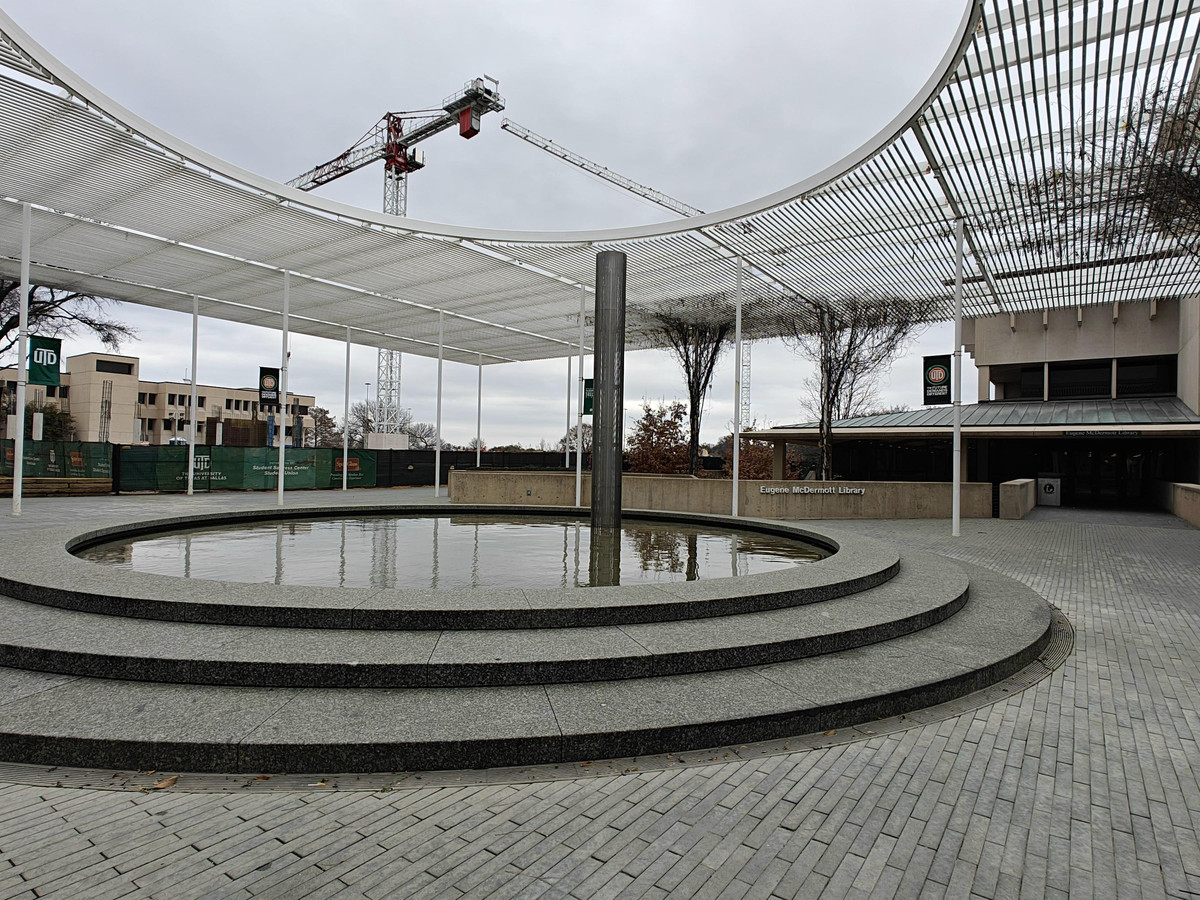
\includegraphics[width=\sw cm,height=\sh cm]{assets/images/appendix/sites/site01.jpg}};
\draw[rpxAccent,line width=.35pt] (0.000,0.000) rectangle ++(\sw,-\sh);
\node[anchor=north west,inner sep=0pt,font=\footnotesize] at (0.000,-3.329) {\textbf{Site 1}\enspace Outdoor};
\node[anchor=north east,inner sep=0pt,font=\fontsize{7.5}{9}\selectfont,text=rpxSlate] at (4.305,-3.329) {scenes 001--005};
\node[anchor=north west,inner sep=0pt,font=\fontsize{7.5}{9}\selectfont,text=rpxSlate] at (0.000,-3.669) {fountain plinth steps};
\node[anchor=north west,inner sep=0pt] at (4.425,0.000) {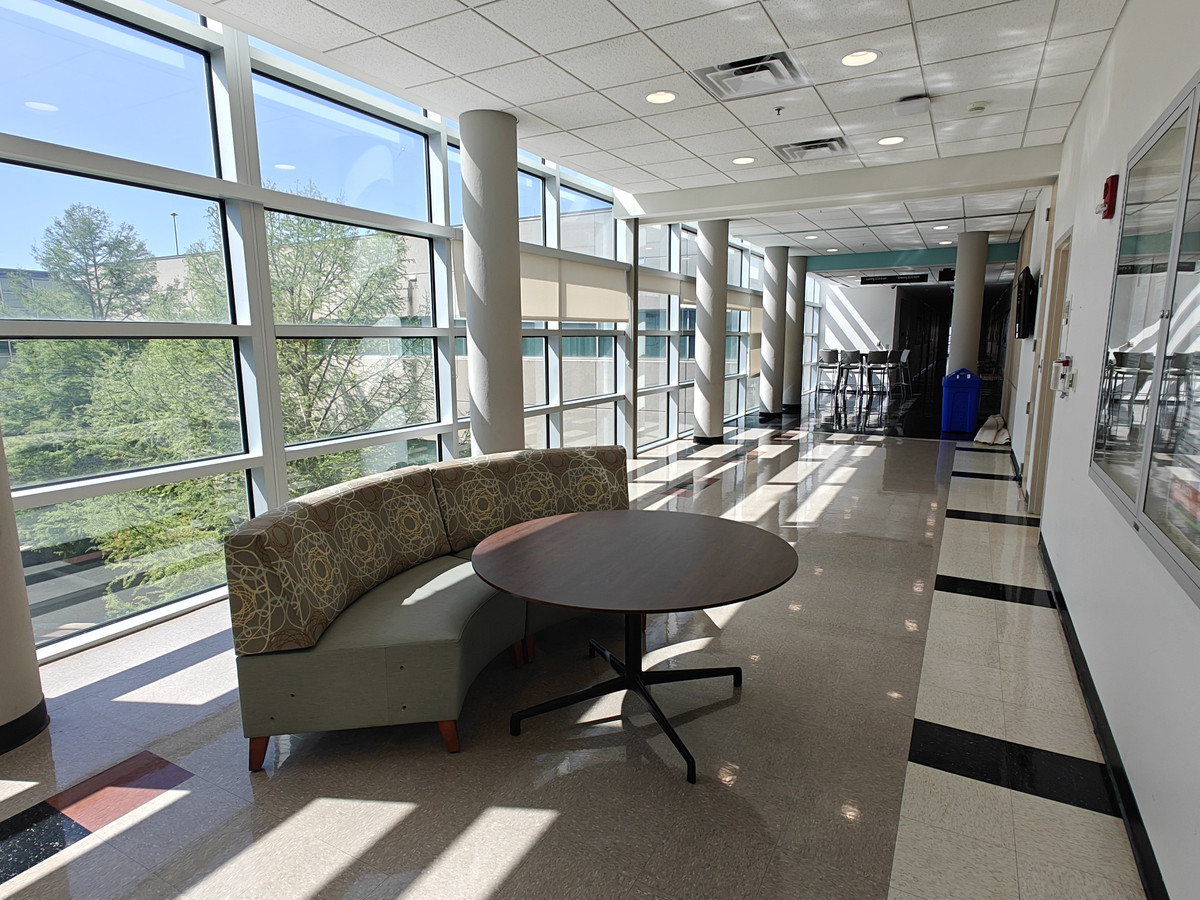
\includegraphics[width=\sw cm,height=\sh cm]{assets/images/appendix/sites/site02.jpg}};
\draw[rpxAccent,line width=.35pt] (4.425,0.000) rectangle ++(\sw,-\sh);
\node[anchor=north west,inner sep=0pt,font=\footnotesize] at (4.425,-3.329) {\textbf{Site 2}\enspace Indoor};
\node[anchor=north east,inner sep=0pt,font=\fontsize{7.5}{9}\selectfont,text=rpxSlate] at (8.730,-3.329) {scenes 006--010};
\node[anchor=north west,inner sep=0pt,font=\fontsize{7.5}{9}\selectfont,text=rpxSlate] at (4.425,-3.669) {round table by windows};
\node[anchor=north west,inner sep=0pt] at (8.850,0.000) {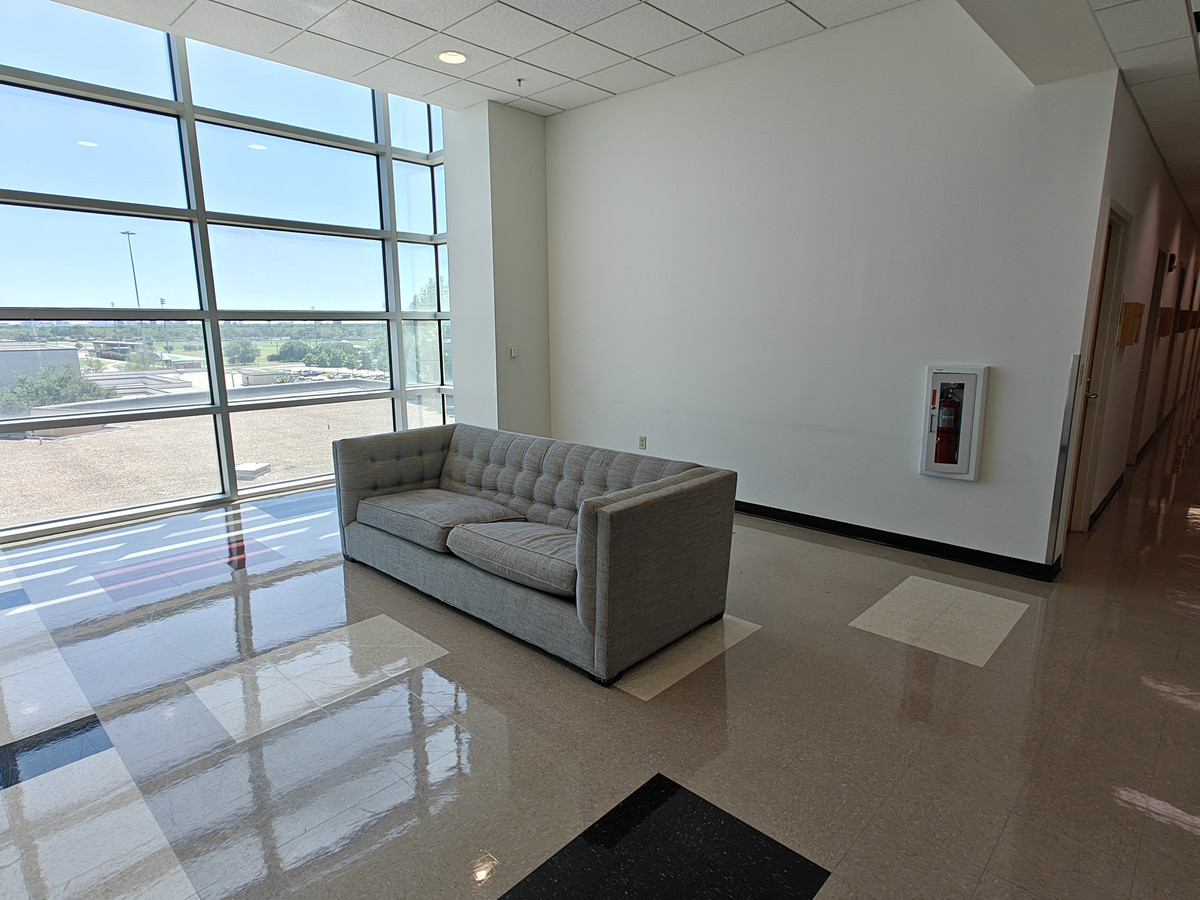
\includegraphics[width=\sw cm,height=\sh cm]{assets/images/appendix/sites/site03.jpg}};
\draw[rpxAccent,line width=.35pt] (8.850,0.000) rectangle ++(\sw,-\sh);
\node[anchor=north west,inner sep=0pt,font=\footnotesize] at (8.850,-3.329) {\textbf{Site 3}\enspace Indoor};
\node[anchor=north east,inner sep=0pt,font=\fontsize{7.5}{9}\selectfont,text=rpxSlate] at (13.155,-3.329) {scenes 011--015};
\node[anchor=north west,inner sep=0pt,font=\fontsize{7.5}{9}\selectfont,text=rpxSlate] at (8.850,-3.669) {sofa lounge};
\node[anchor=north west,inner sep=0pt] at (13.275,0.000) {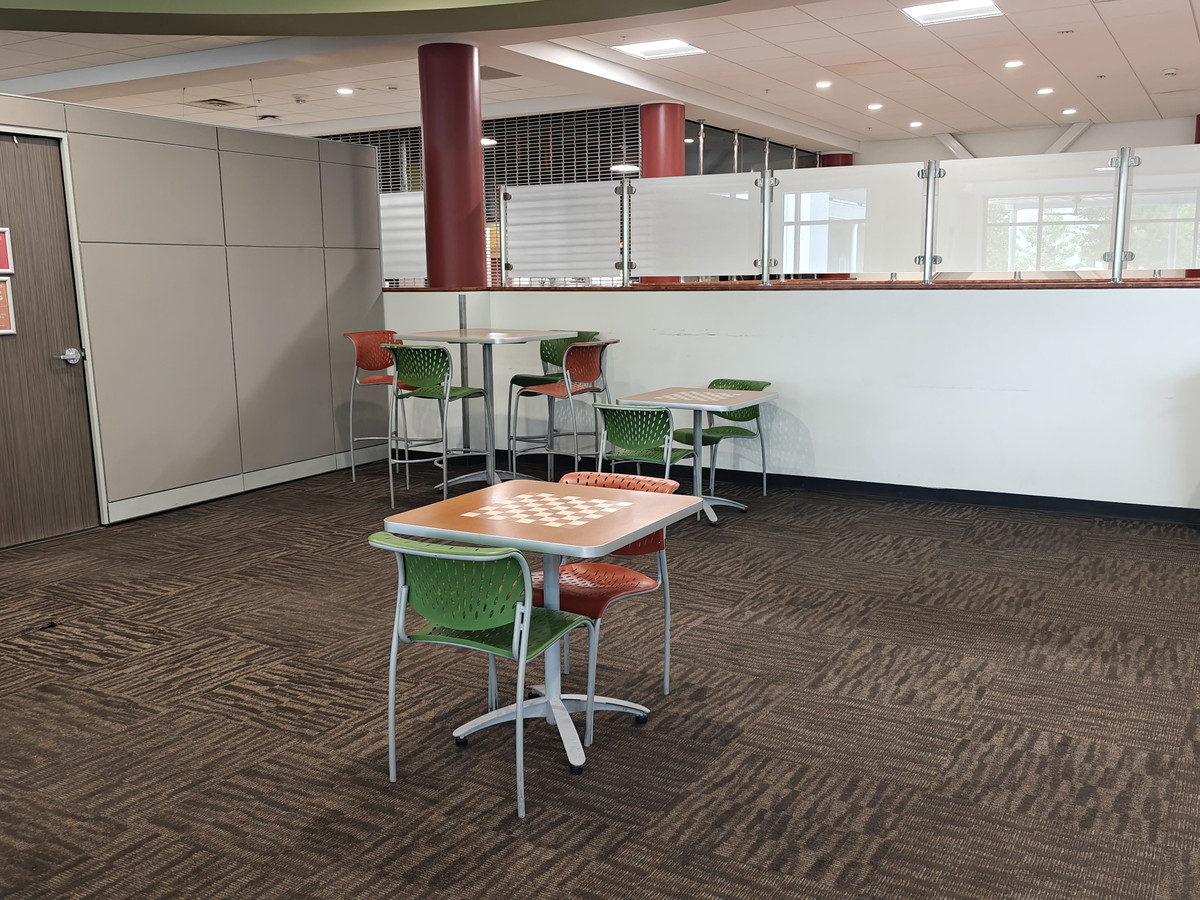
\includegraphics[width=\sw cm,height=\sh cm]{assets/images/appendix/sites/site04.jpg}};
\draw[rpxAccent,line width=.35pt] (13.275,0.000) rectangle ++(\sw,-\sh);
\node[anchor=north west,inner sep=0pt,font=\footnotesize] at (13.275,-3.329) {\textbf{Site 4}\enspace Indoor};
\node[anchor=north east,inner sep=0pt,font=\fontsize{7.5}{9}\selectfont,text=rpxSlate] at (17.580,-3.329) {scenes 016--020};
\node[anchor=north west,inner sep=0pt,font=\fontsize{7.5}{9}\selectfont,text=rpxSlate] at (13.275,-3.669) {checkerboard dining table};
\node[anchor=north west,inner sep=0pt] at (0.000,-4.009) {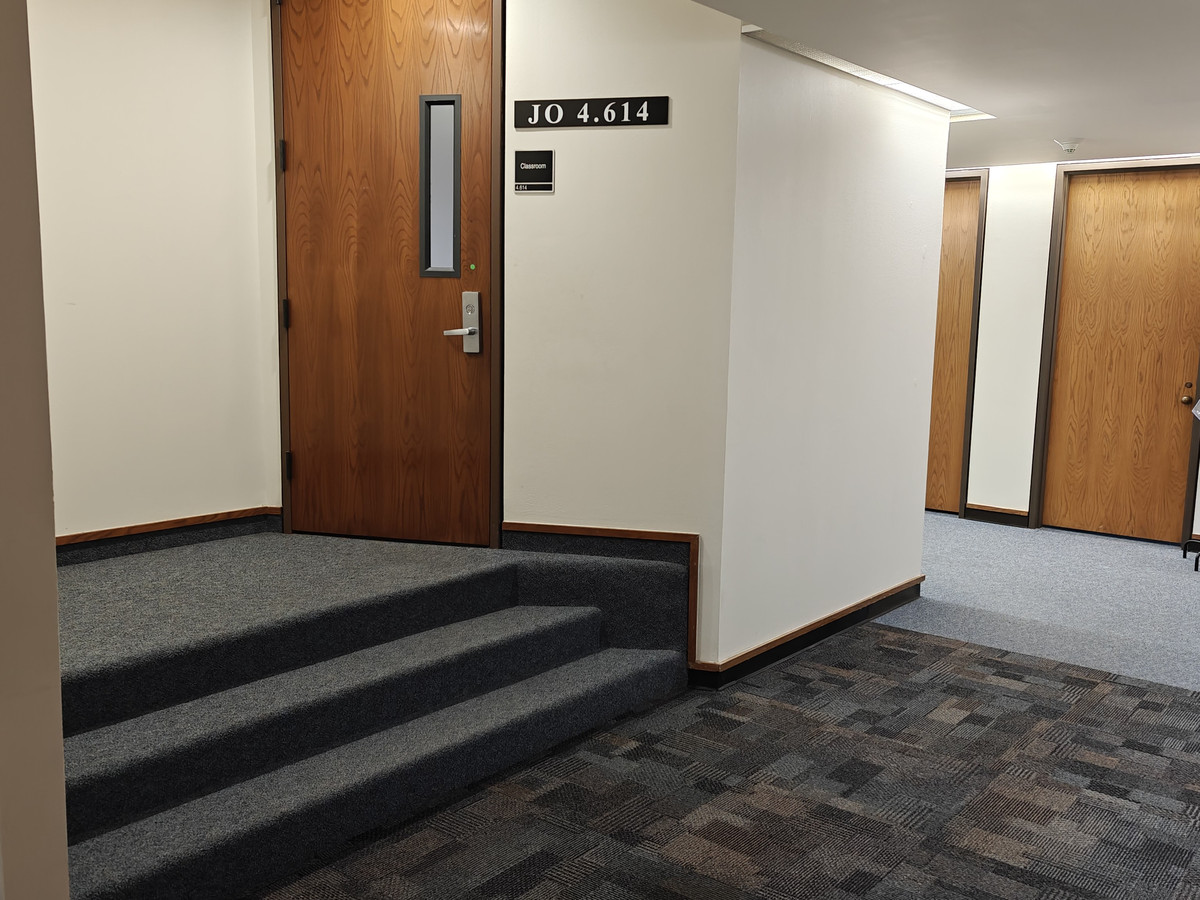
\includegraphics[width=\sw cm,height=\sh cm]{assets/images/appendix/sites/site05.jpg}};
\draw[rpxAccent,line width=.35pt] (0.000,-4.009) rectangle ++(\sw,-\sh);
\node[anchor=north west,inner sep=0pt,font=\footnotesize] at (0.000,-7.338) {\textbf{Site 5}\enspace Indoor};
\node[anchor=north east,inner sep=0pt,font=\fontsize{7.5}{9}\selectfont,text=rpxSlate] at (4.305,-7.338) {scenes 021--025};
\node[anchor=north west,inner sep=0pt,font=\fontsize{7.5}{9}\selectfont,text=rpxSlate] at (0.000,-7.678) {carpeted stairs};
\node[anchor=north west,inner sep=0pt] at (4.425,-4.009) {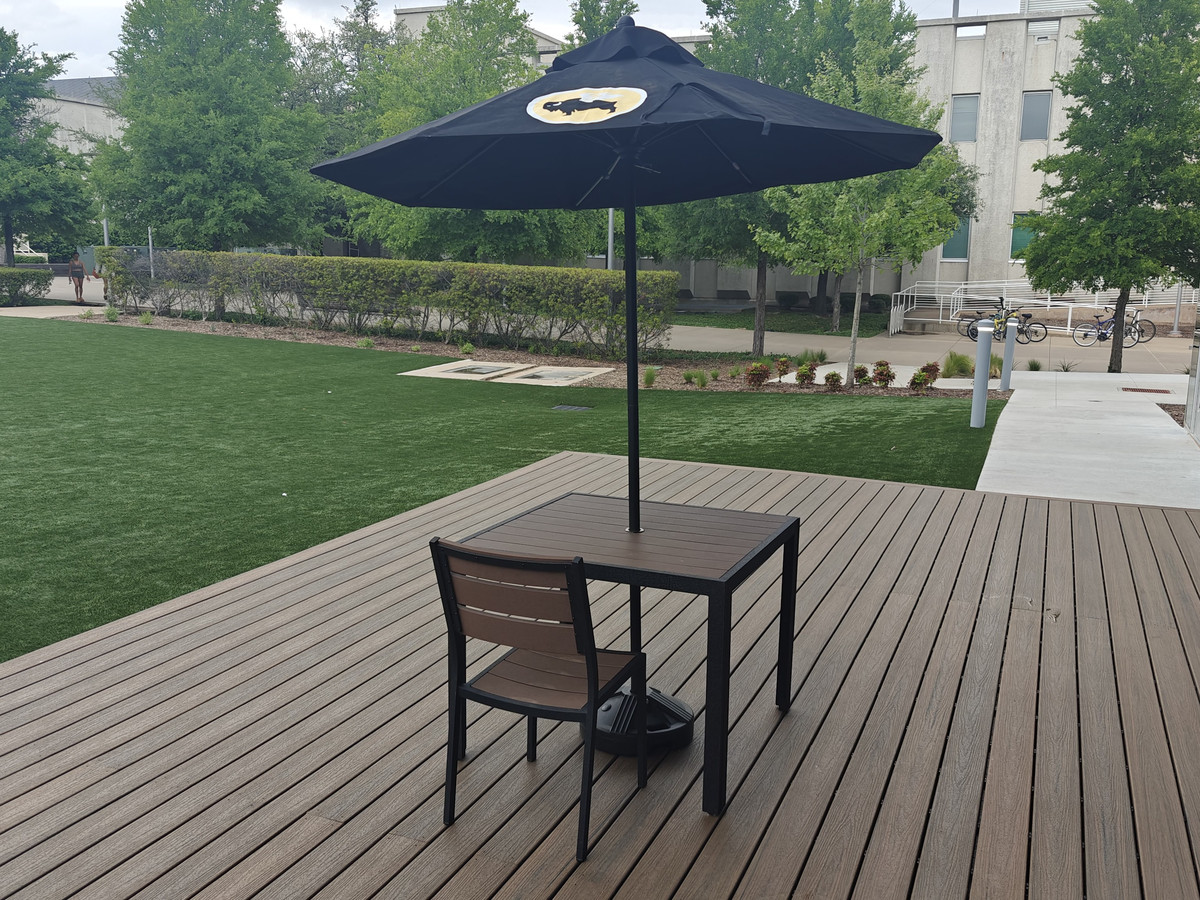
\includegraphics[width=\sw cm,height=\sh cm]{assets/images/appendix/sites/site06.jpg}};
\draw[rpxAccent,line width=.35pt] (4.425,-4.009) rectangle ++(\sw,-\sh);
\node[anchor=north west,inner sep=0pt,font=\footnotesize] at (4.425,-7.338) {\textbf{Site 6}\enspace Outdoor};
\node[anchor=north east,inner sep=0pt,font=\fontsize{7.5}{9}\selectfont,text=rpxSlate] at (8.730,-7.338) {scenes 026--030};
\node[anchor=north west,inner sep=0pt,font=\fontsize{7.5}{9}\selectfont,text=rpxSlate] at (4.425,-7.678) {deck table with umbrella};
\node[anchor=north west,inner sep=0pt] at (8.850,-4.009) {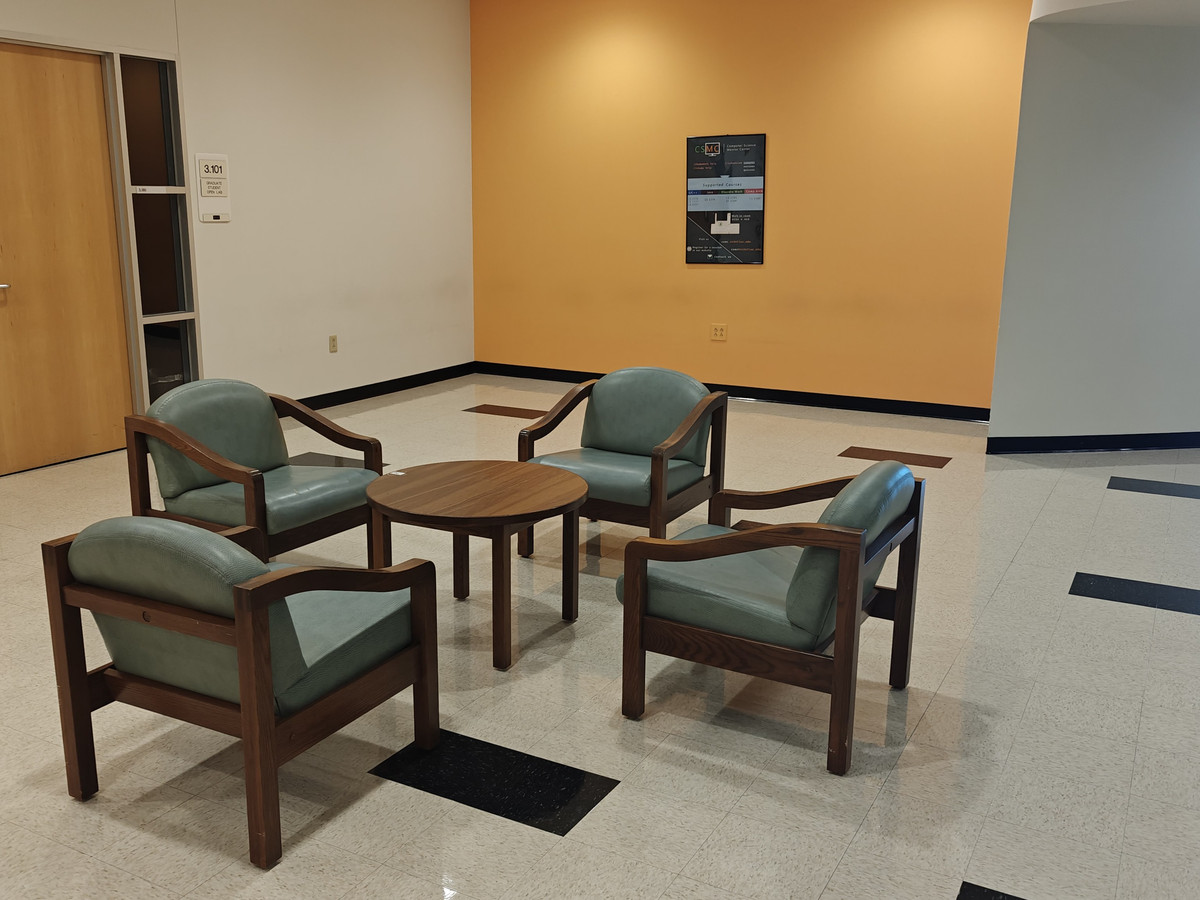
\includegraphics[width=\sw cm,height=\sh cm]{assets/images/appendix/sites/site07.jpg}};
\draw[rpxAccent,line width=.35pt] (8.850,-4.009) rectangle ++(\sw,-\sh);
\node[anchor=north west,inner sep=0pt,font=\footnotesize] at (8.850,-7.338) {\textbf{Site 7}\enspace Indoor};
\node[anchor=north east,inner sep=0pt,font=\fontsize{7.5}{9}\selectfont,text=rpxSlate] at (13.155,-7.338) {scenes 031--035};
\node[anchor=north west,inner sep=0pt,font=\fontsize{7.5}{9}\selectfont,text=rpxSlate] at (8.850,-7.678) {sitting area};
\node[anchor=north west,inner sep=0pt] at (13.275,-4.009) {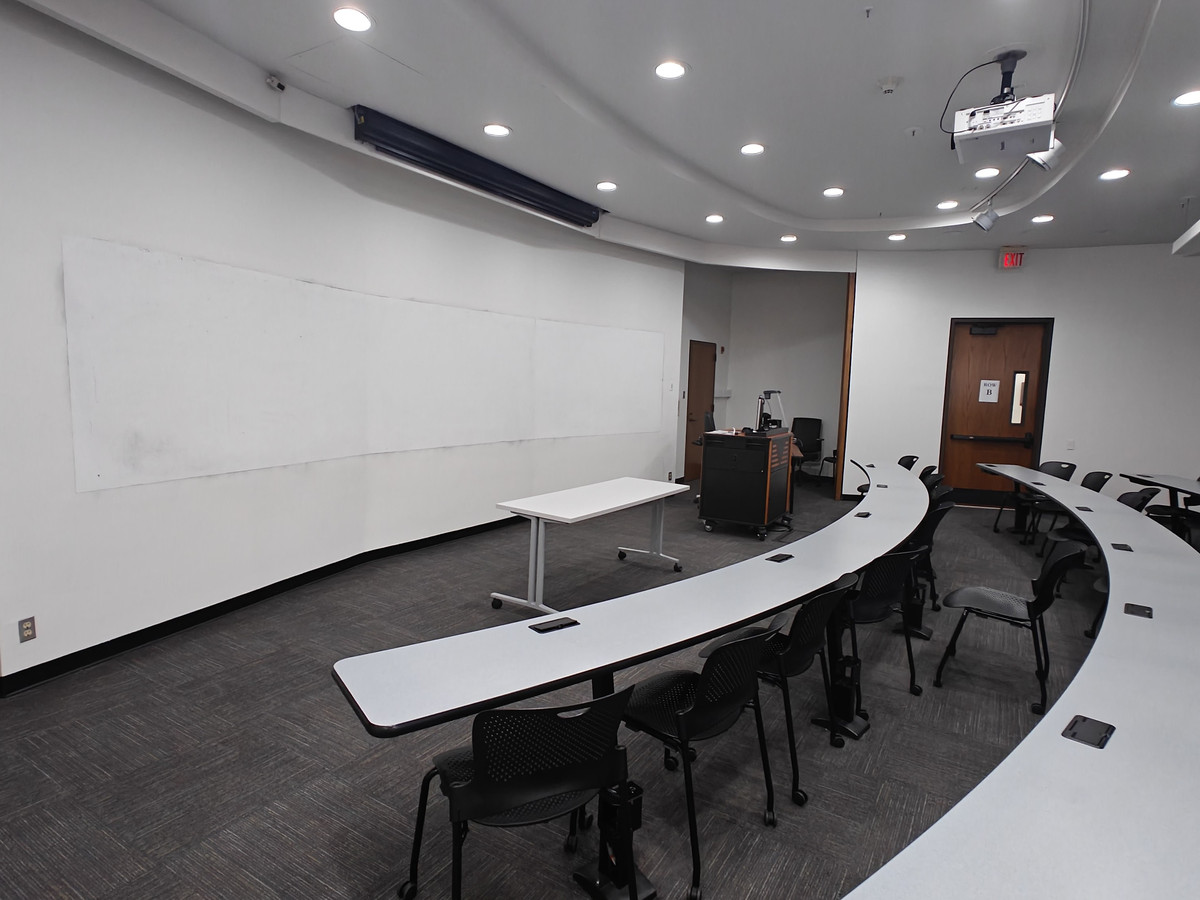
\includegraphics[width=\sw cm,height=\sh cm]{assets/images/appendix/sites/site08.jpg}};
\draw[rpxAccent,line width=.35pt] (13.275,-4.009) rectangle ++(\sw,-\sh);
\node[anchor=north west,inner sep=0pt,font=\footnotesize] at (13.275,-7.338) {\textbf{Site 8}\enspace Indoor};
\node[anchor=north east,inner sep=0pt,font=\fontsize{7.5}{9}\selectfont,text=rpxSlate] at (17.580,-7.338) {scenes 036--040};
\node[anchor=north west,inner sep=0pt,font=\fontsize{7.5}{9}\selectfont,text=rpxSlate] at (13.275,-7.678) {lecture hall table};
\node[anchor=north west,inner sep=0pt] at (0.000,-8.018) {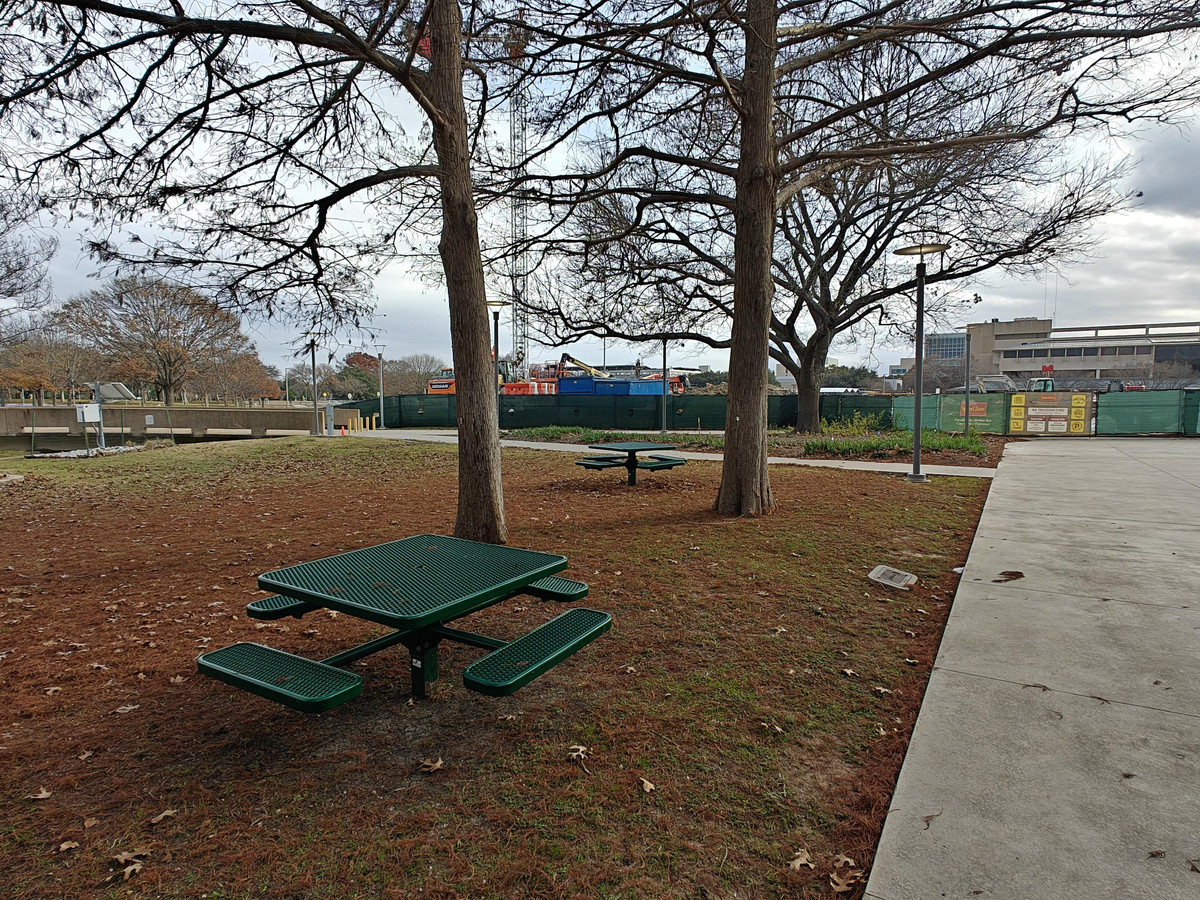
\includegraphics[width=\sw cm,height=\sh cm]{assets/images/appendix/sites/site09.jpg}};
\draw[rpxAccent,line width=.35pt] (0.000,-8.018) rectangle ++(\sw,-\sh);
\node[anchor=north west,inner sep=0pt,font=\footnotesize] at (0.000,-11.347) {\textbf{Site 9}\enspace Outdoor};
\node[anchor=north east,inner sep=0pt,font=\fontsize{7.5}{9}\selectfont,text=rpxSlate] at (4.305,-11.347) {scenes 041--045};
\node[anchor=north west,inner sep=0pt,font=\fontsize{7.5}{9}\selectfont,text=rpxSlate] at (0.000,-11.687) {picnic bench};
\node[anchor=north west,inner sep=0pt] at (4.425,-8.018) {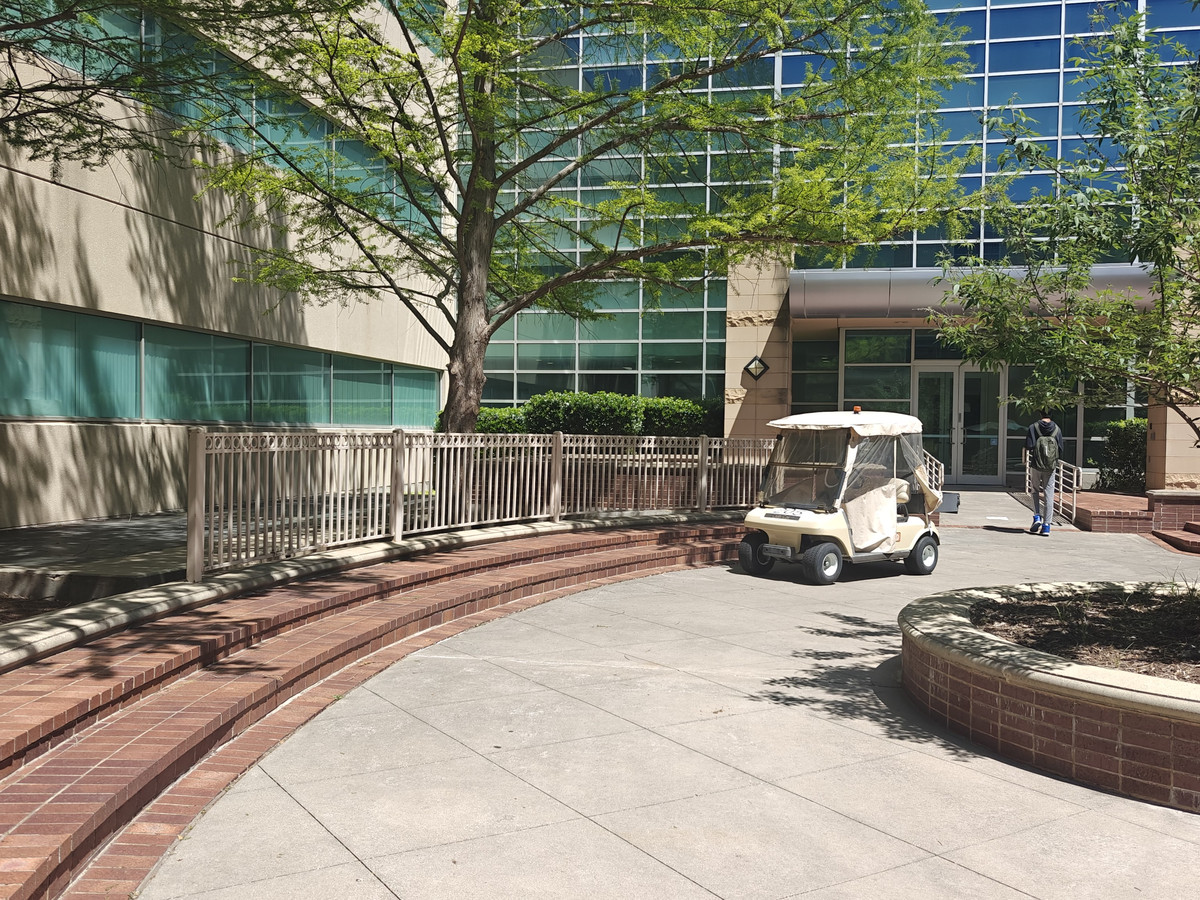
\includegraphics[width=\sw cm,height=\sh cm]{assets/images/appendix/sites/site10.jpg}};
\draw[rpxAccent,line width=.35pt] (4.425,-8.018) rectangle ++(\sw,-\sh);
\node[anchor=north west,inner sep=0pt,font=\footnotesize] at (4.425,-11.347) {\textbf{Site 10}\enspace Outdoor};
\node[anchor=north east,inner sep=0pt,font=\fontsize{7.5}{9}\selectfont,text=rpxSlate] at (8.730,-11.347) {scenes 046--050};
\node[anchor=north west,inner sep=0pt,font=\fontsize{7.5}{9}\selectfont,text=rpxSlate] at (4.425,-11.687) {shaded brick steps};
\node[anchor=north west,inner sep=0pt] at (8.850,-8.018) {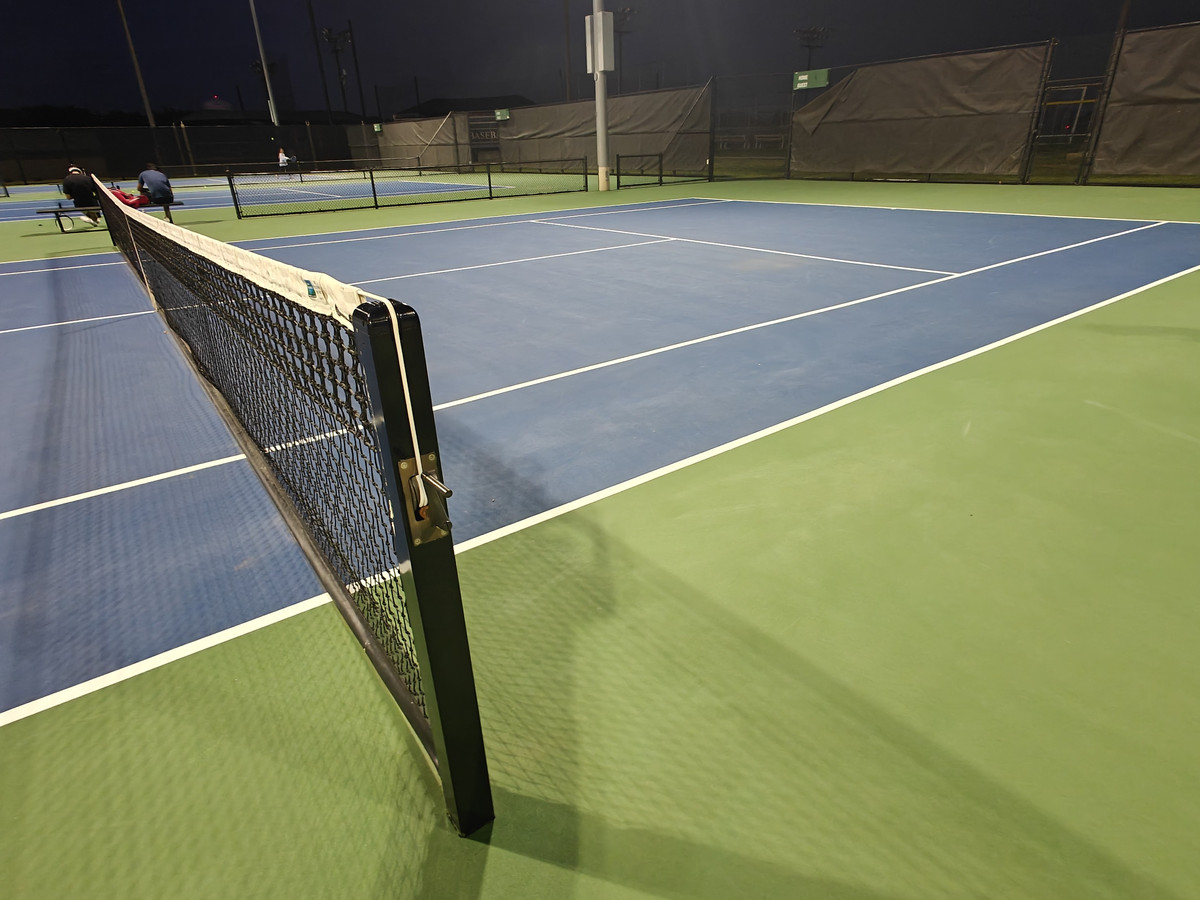
\includegraphics[width=\sw cm,height=\sh cm]{assets/images/appendix/sites/site11.jpg}};
\draw[rpxAccent,line width=.35pt] (8.850,-8.018) rectangle ++(\sw,-\sh);
\node[anchor=north west,inner sep=0pt,font=\footnotesize] at (8.850,-11.347) {\textbf{Site 11}\enspace Outdoor};
\node[anchor=north east,inner sep=0pt,font=\fontsize{7.5}{9}\selectfont,text=rpxSlate] at (13.155,-11.347) {scenes 051--055};
\node[anchor=north west,inner sep=0pt,font=\fontsize{7.5}{9}\selectfont,text=rpxSlate] at (8.850,-11.687) {tennis court};
\node[anchor=north west,inner sep=0pt] at (13.275,-8.018) {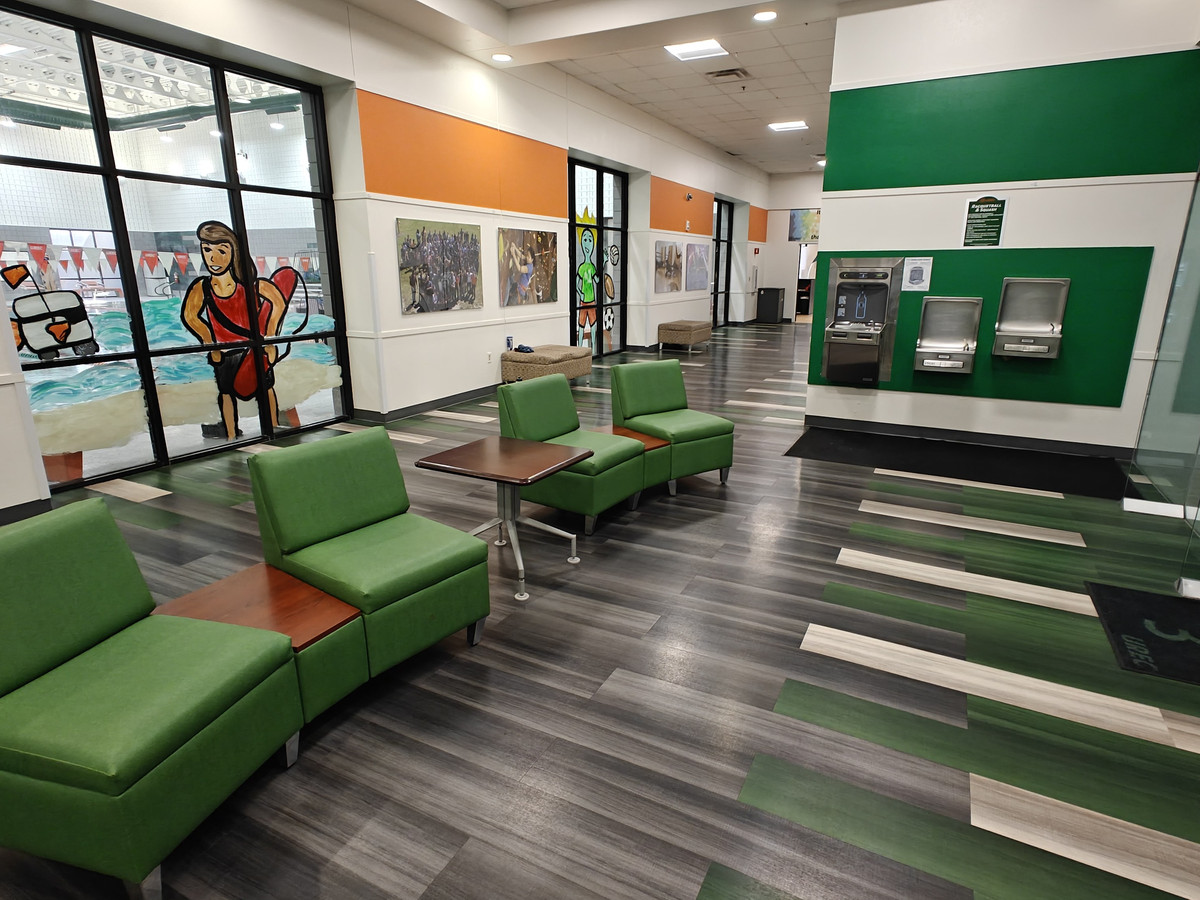
\includegraphics[width=\sw cm,height=\sh cm]{assets/images/appendix/sites/site12.jpg}};
\draw[rpxAccent,line width=.35pt] (13.275,-8.018) rectangle ++(\sw,-\sh);
\node[anchor=north west,inner sep=0pt,font=\footnotesize] at (13.275,-11.347) {\textbf{Site 12}\enspace Indoor};
\node[anchor=north east,inner sep=0pt,font=\fontsize{7.5}{9}\selectfont,text=rpxSlate] at (17.580,-11.347) {scenes 056--060};
\node[anchor=north west,inner sep=0pt,font=\fontsize{7.5}{9}\selectfont,text=rpxSlate] at (13.275,-11.687) {lounge benches};
\node[anchor=north west,inner sep=0pt] at (0.000,-12.027) {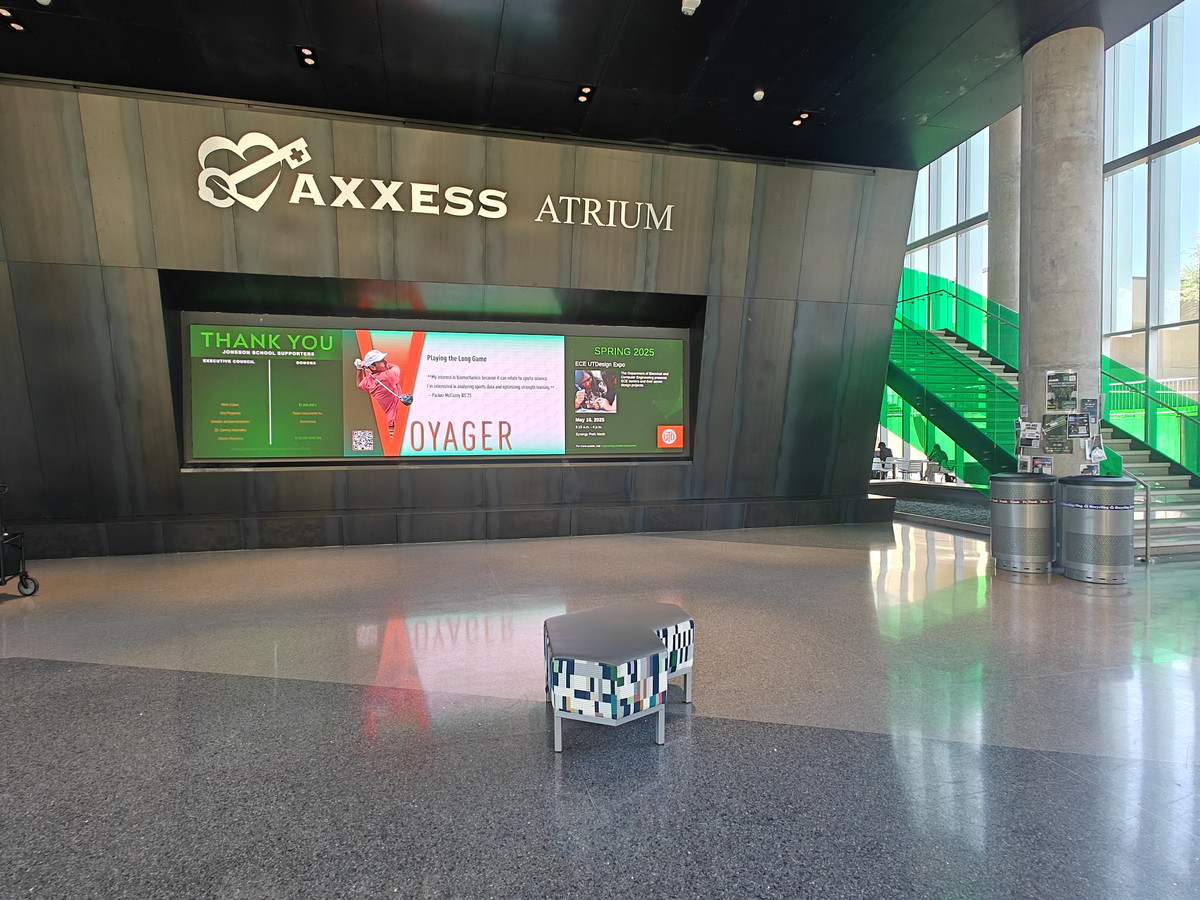
\includegraphics[width=\sw cm,height=\sh cm]{assets/images/appendix/sites/site13.jpg}};
\draw[rpxAccent,line width=.35pt] (0.000,-12.027) rectangle ++(\sw,-\sh);
\node[anchor=north west,inner sep=0pt,font=\footnotesize] at (0.000,-15.356) {\textbf{Site 13}\enspace Indoor};
\node[anchor=north east,inner sep=0pt,font=\fontsize{7.5}{9}\selectfont,text=rpxSlate] at (4.305,-15.356) {scenes 061--065};
\node[anchor=north west,inner sep=0pt,font=\fontsize{7.5}{9}\selectfont,text=rpxSlate] at (0.000,-15.696) {atrium seating block};
\node[anchor=north west,inner sep=0pt] at (4.425,-12.027) {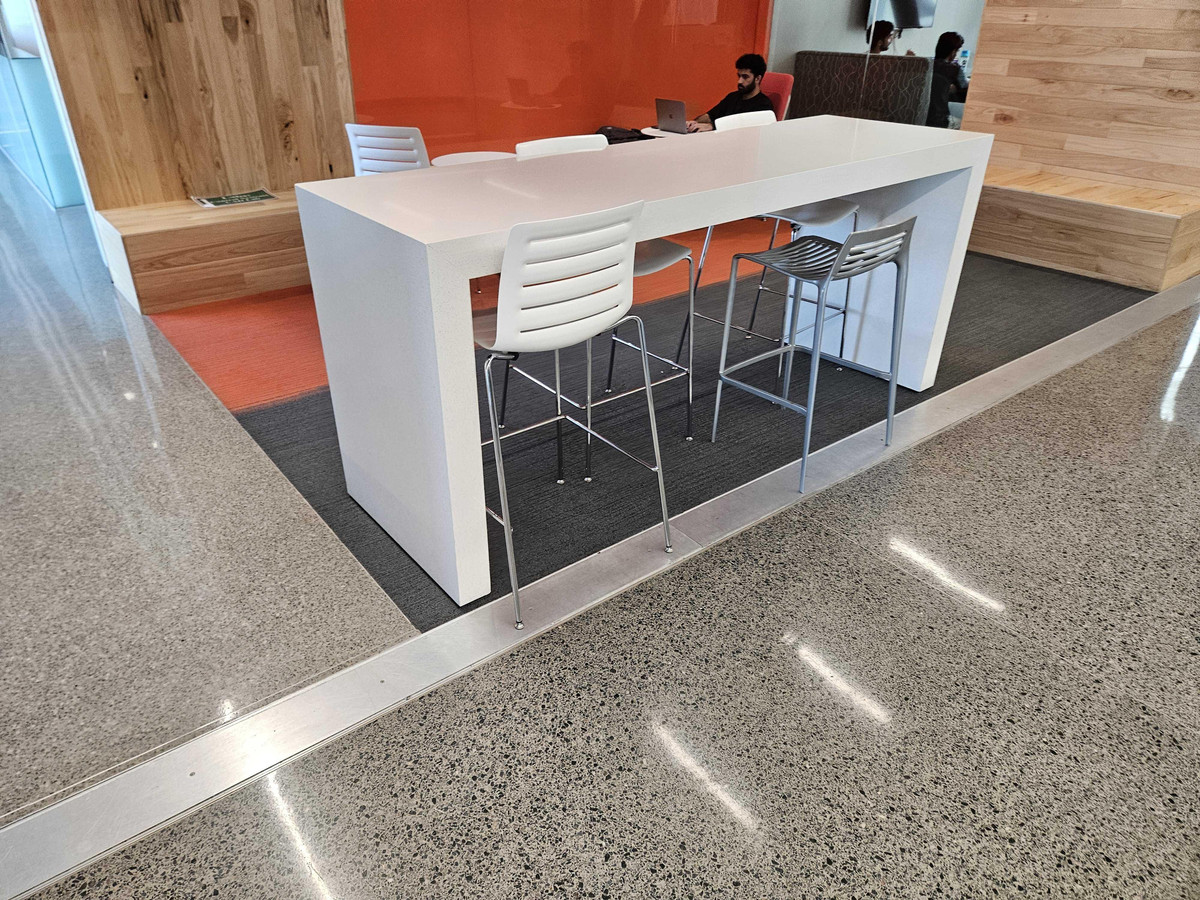
\includegraphics[width=\sw cm,height=\sh cm]{assets/images/appendix/sites/site14.jpg}};
\draw[rpxAccent,line width=.35pt] (4.425,-12.027) rectangle ++(\sw,-\sh);
\node[anchor=north west,inner sep=0pt,font=\footnotesize] at (4.425,-15.356) {\textbf{Site 14}\enspace Indoor};
\node[anchor=north east,inner sep=0pt,font=\fontsize{7.5}{9}\selectfont,text=rpxSlate] at (8.730,-15.356) {scenes 066--070};
\node[anchor=north west,inner sep=0pt,font=\fontsize{7.5}{9}\selectfont,text=rpxSlate] at (4.425,-15.696) {tall white table};
\node[anchor=north west,inner sep=0pt] at (8.850,-12.027) {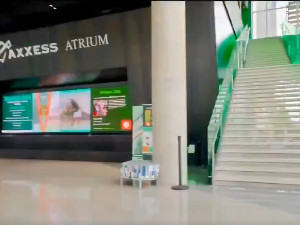
\includegraphics[width=\sw cm,height=\sh cm]{assets/images/appendix/sites/site15.jpg}};
\draw[rpxAccent,line width=.35pt] (8.850,-12.027) rectangle ++(\sw,-\sh);
\node[anchor=north west,inner sep=0pt,font=\footnotesize] at (8.850,-15.356) {\textbf{Site 15}\enspace Indoor};
\node[anchor=north east,inner sep=0pt,font=\fontsize{7.5}{9}\selectfont,text=rpxSlate] at (13.155,-15.356) {scenes 071--075};
\node[anchor=north west,inner sep=0pt,font=\fontsize{7.5}{9}\selectfont,text=rpxSlate] at (8.850,-15.696) {atrium stairs};
\node[anchor=north west,inner sep=0pt] at (13.275,-12.027) {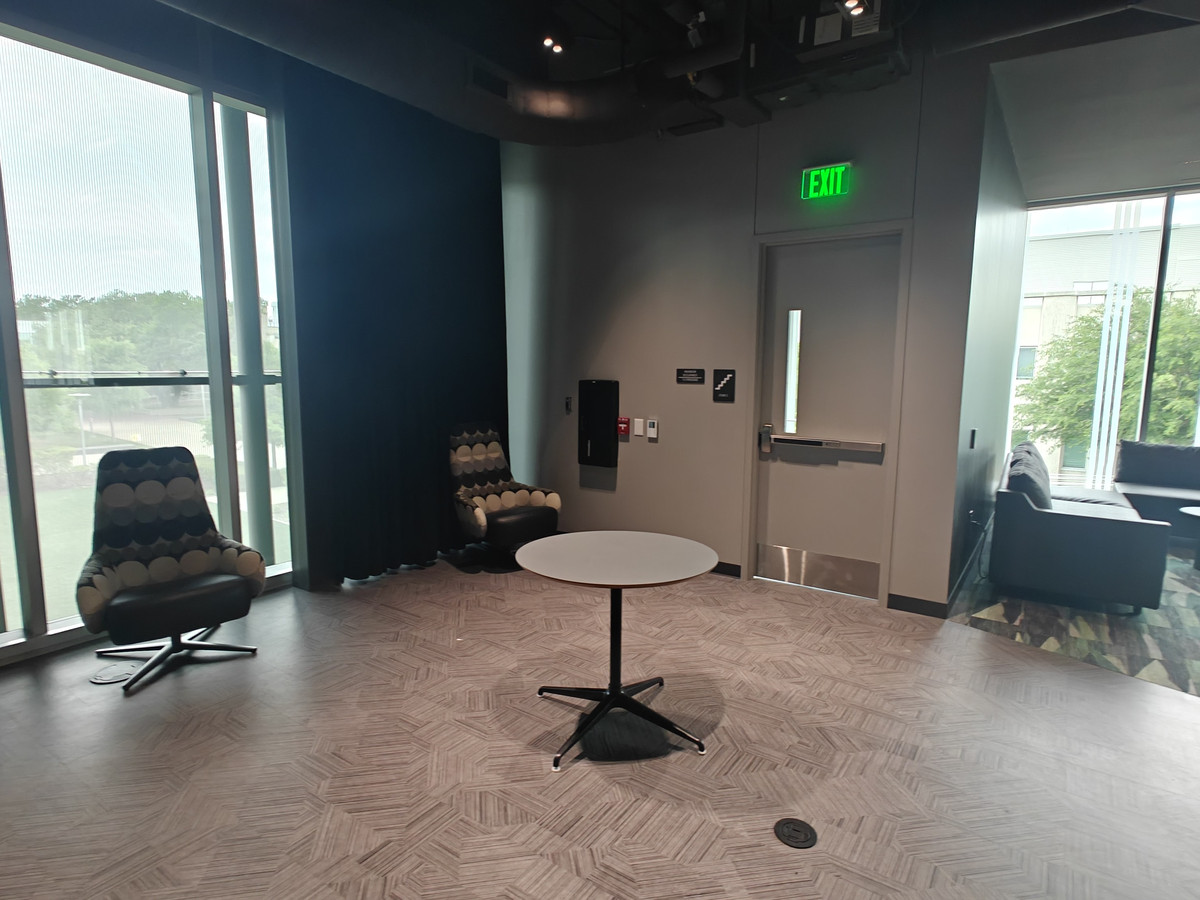
\includegraphics[width=\sw cm,height=\sh cm]{assets/images/appendix/sites/site16.jpg}};
\draw[rpxAccent,line width=.35pt] (13.275,-12.027) rectangle ++(\sw,-\sh);
\node[anchor=north west,inner sep=0pt,font=\footnotesize] at (13.275,-15.356) {\textbf{Site 16}\enspace Indoor};
\node[anchor=north east,inner sep=0pt,font=\fontsize{7.5}{9}\selectfont,text=rpxSlate] at (17.580,-15.356) {scenes 076--080};
\node[anchor=north west,inner sep=0pt,font=\fontsize{7.5}{9}\selectfont,text=rpxSlate] at (13.275,-15.696) {round lounge table};
\node[anchor=north west,inner sep=0pt] at (0.000,-16.036) {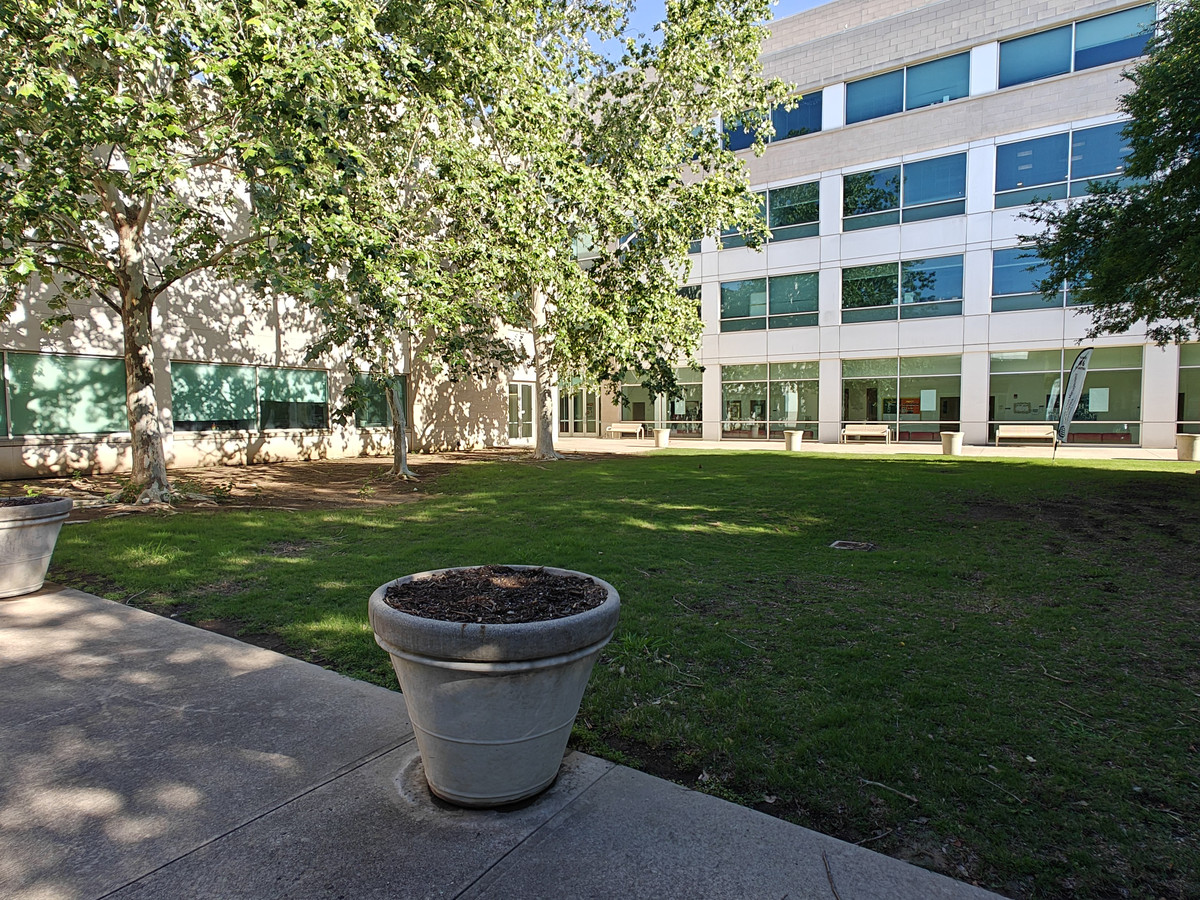
\includegraphics[width=\sw cm,height=\sh cm]{assets/images/appendix/sites/site17.jpg}};
\draw[rpxAccent,line width=.35pt] (0.000,-16.036) rectangle ++(\sw,-\sh);
\node[anchor=north west,inner sep=0pt,font=\footnotesize] at (0.000,-19.365) {\textbf{Site 17}\enspace Outdoor};
\node[anchor=north east,inner sep=0pt,font=\fontsize{7.5}{9}\selectfont,text=rpxSlate] at (4.305,-19.365) {scenes 081--085};
\node[anchor=north west,inner sep=0pt,font=\fontsize{7.5}{9}\selectfont,text=rpxSlate] at (0.000,-19.705) {garden planter};
\node[anchor=north west,inner sep=0pt] at (4.425,-16.036) {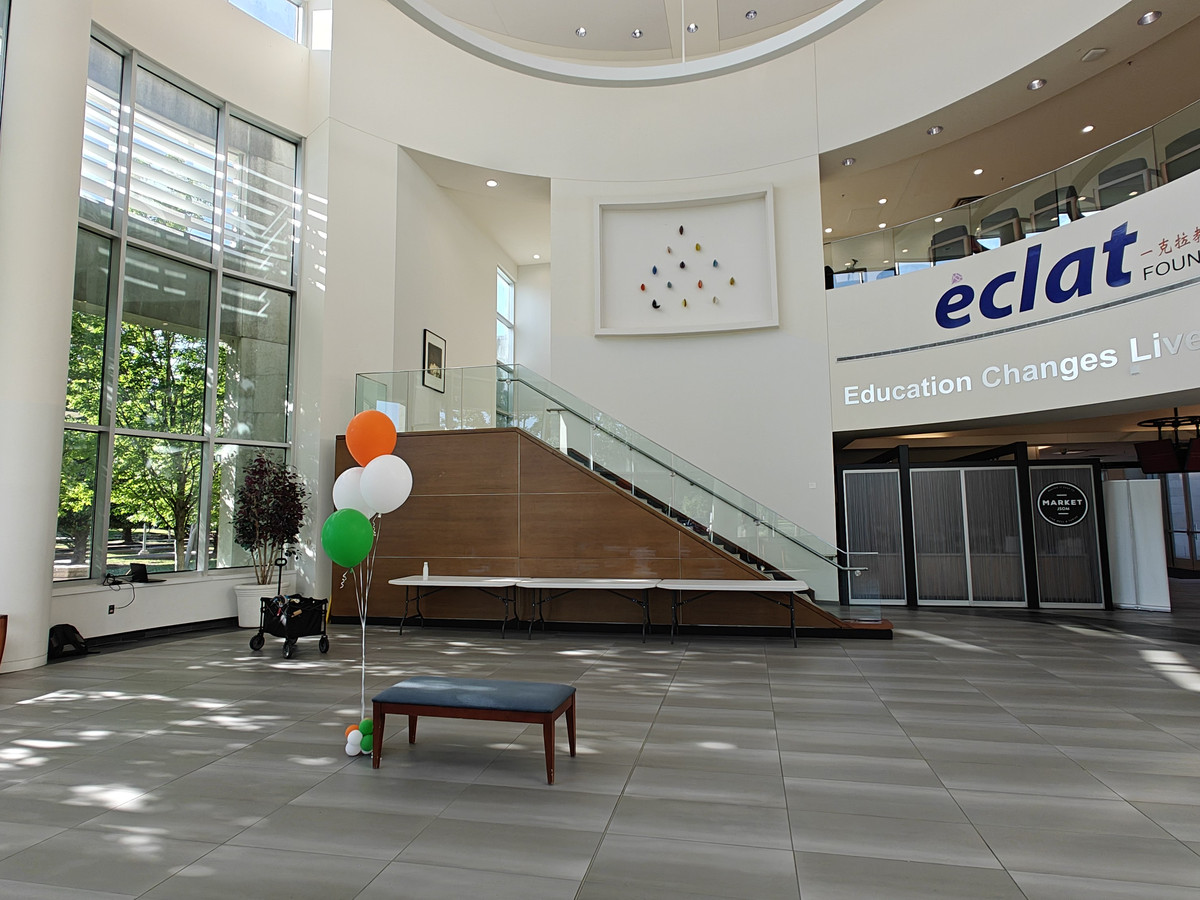
\includegraphics[width=\sw cm,height=\sh cm]{assets/images/appendix/sites/site18.jpg}};
\draw[rpxAccent,line width=.35pt] (4.425,-16.036) rectangle ++(\sw,-\sh);
\node[anchor=north west,inner sep=0pt,font=\footnotesize] at (4.425,-19.365) {\textbf{Site 18}\enspace Indoor};
\node[anchor=north east,inner sep=0pt,font=\fontsize{7.5}{9}\selectfont,text=rpxSlate] at (8.730,-19.365) {scenes 086--090};
\node[anchor=north west,inner sep=0pt,font=\fontsize{7.5}{9}\selectfont,text=rpxSlate] at (4.425,-19.705) {atrium bench};
\node[anchor=north west,inner sep=0pt] at (8.850,-16.036) {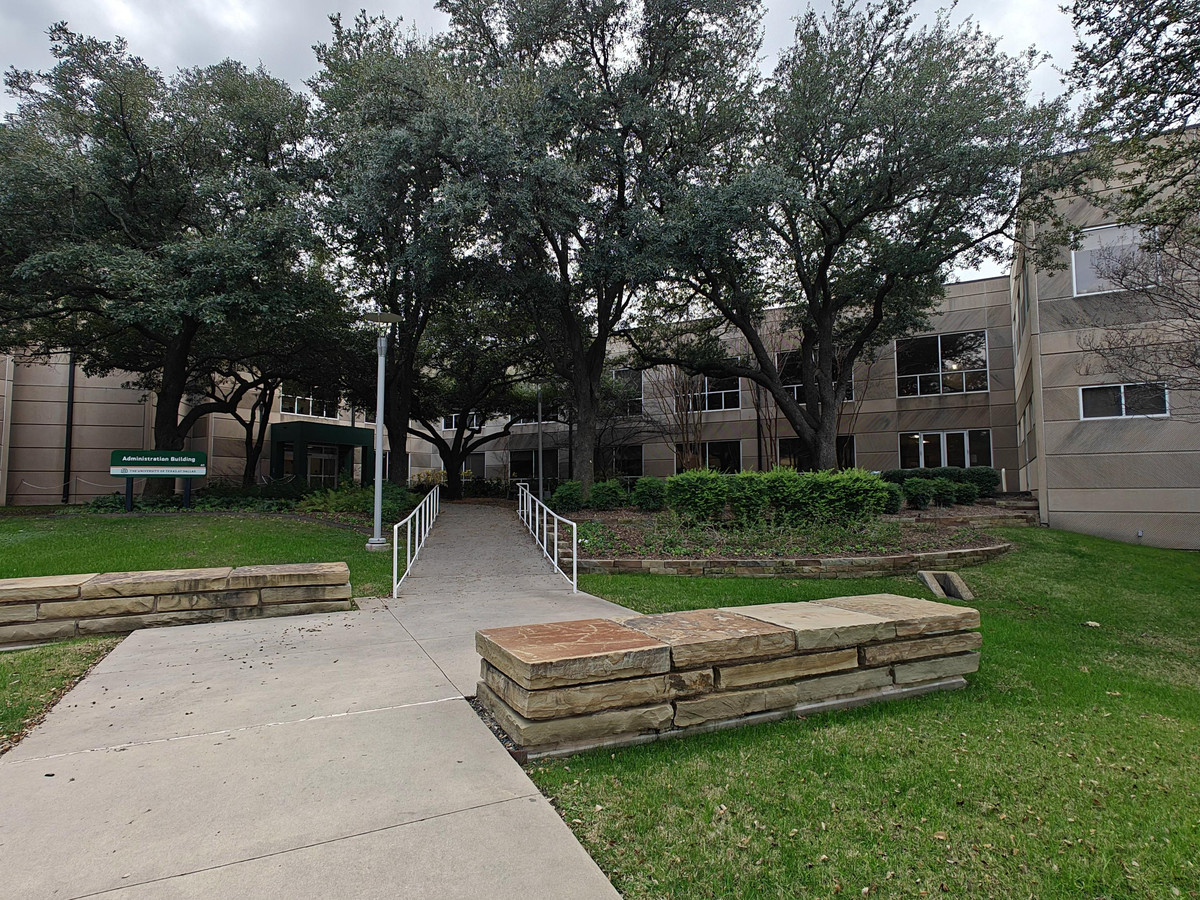
\includegraphics[width=\sw cm,height=\sh cm]{assets/images/appendix/sites/site19.jpg}};
\draw[rpxAccent,line width=.35pt] (8.850,-16.036) rectangle ++(\sw,-\sh);
\node[anchor=north west,inner sep=0pt,font=\footnotesize] at (8.850,-19.365) {\textbf{Site 19}\enspace Outdoor};
\node[anchor=north east,inner sep=0pt,font=\fontsize{7.5}{9}\selectfont,text=rpxSlate] at (13.155,-19.365) {scenes 091--095};
\node[anchor=north west,inner sep=0pt,font=\fontsize{7.5}{9}\selectfont,text=rpxSlate] at (8.850,-19.705) {stone bench};
\node[anchor=north west,inner sep=0pt] at (13.275,-16.036) {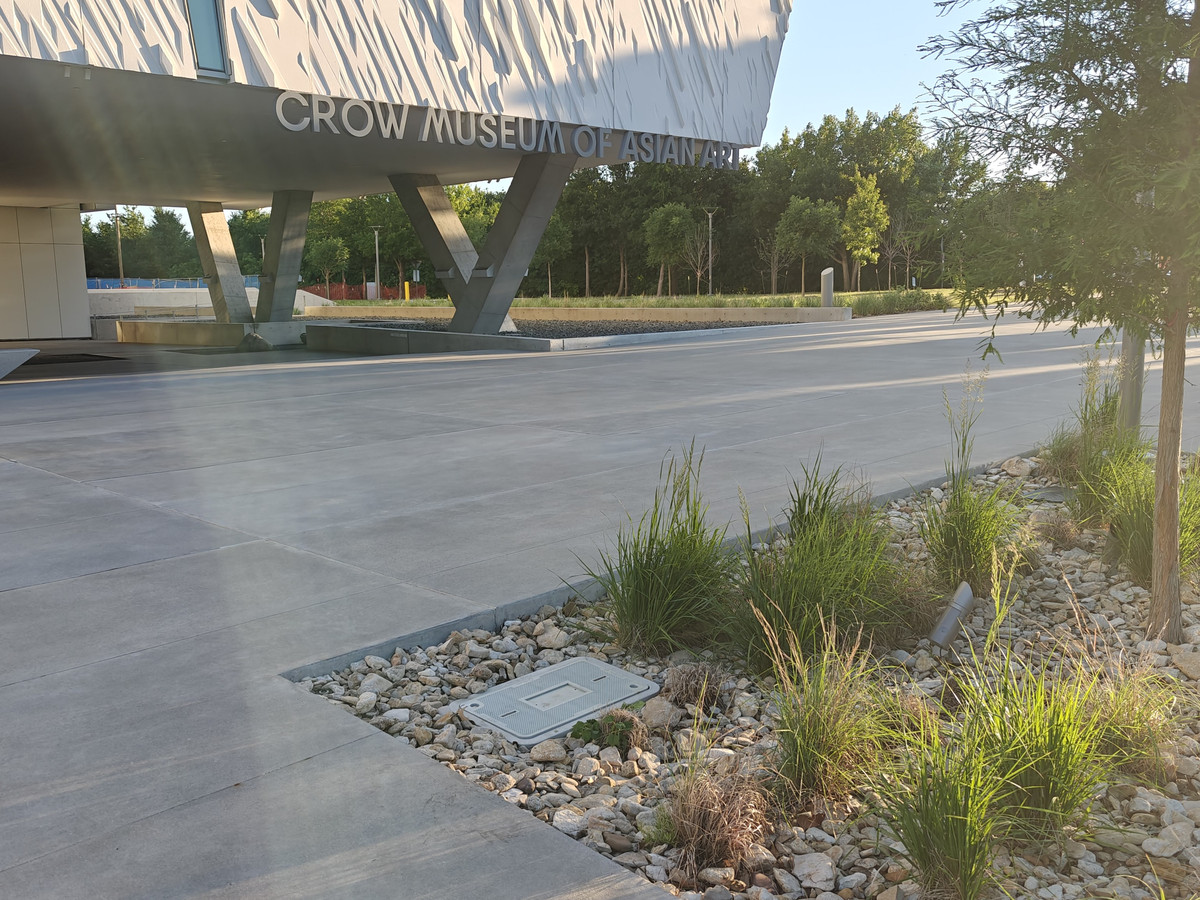
\includegraphics[width=\sw cm,height=\sh cm]{assets/images/appendix/sites/site20.jpg}};
\draw[rpxAccent,line width=.35pt] (13.275,-16.036) rectangle ++(\sw,-\sh);
\node[anchor=north west,inner sep=0pt,font=\footnotesize] at (13.275,-19.365) {\textbf{Site 20}\enspace Outdoor};
\node[anchor=north east,inner sep=0pt,font=\fontsize{7.5}{9}\selectfont,text=rpxSlate] at (17.580,-19.365) {scenes 096--100};
\node[anchor=north west,inner sep=0pt,font=\fontsize{7.5}{9}\selectfont,text=rpxSlate] at (13.275,-19.705) {rock garden};
\end{tikzpicture}

\caption{The 20 capture sites, photographed without the scene objects. Each site hosts five consecutive MOS scenes.}
\label{fig:appendix-capture-sites}
\end{figure*}

\subsection{Complete scene inventory}

Figure~\ref{fig:appendix-scene-catalogue} shows all 100 MOS scenes in scene order, one scene per row, with the environment and difficulty group of the scene. Every view uses the same selection rule: the middle frame (index $\lfloor n/2\rfloor$ of the $n$ frames) of that capture, shown as recorded without masks. These frames summarize the scene visually and have no special role in evaluation.

% Generated by tools/catalogue_frames/build_scene_catalogue.py -- do not edit by hand.
\begin{figure*}[p]
\centering\catheader
\setlength\catRowSep{\catG}
\catrow{001}{Outdoor}{tierH}{Hard}
\catrow{002}{Outdoor}{tierH}{Hard}
\catrow{003}{Outdoor}{tierH}{Hard}
\catrow{004}{Outdoor}{tierE}{Easy}
\catrow{005}{Outdoor}{tierH}{Hard}
\catrow{006}{Indoor}{tierM}{Medium}
\catrow{007}{Indoor}{tierM}{Medium}
\catrow{008}{Indoor}{tierE}{Easy}
\caption{Complete multi-object scene catalogue, scenes 001--008. Each row shows the middle frame of the Clutter, Interaction, and Clean exocentric captures and of the egocentric Interaction clip.}
\label{fig:appendix-scene-catalogue}
\end{figure*}
\begin{figure*}[p]
\ContinuedFloat
\centering\catheader
\setlength\catRowSep{\catG}
\catrow{009}{Indoor}{tierM}{Medium}
\catrow{010}{Indoor}{tierH}{Hard}
\catrow{011}{Indoor}{tierE}{Easy}
\catrow{012}{Indoor}{tierE}{Easy}
\catrow{013}{Indoor}{tierE}{Easy}
\catrow{014}{Indoor}{tierM}{Medium}
\catrow{015}{Indoor}{tierE}{Easy}
\catrow{016}{Indoor}{tierH}{Hard}
\caption[]{Complete multi-object scene catalogue (continued), scenes 009--016.}
\end{figure*}
\begin{figure*}[p]
\ContinuedFloat
\centering\catheader
\setlength\catRowSep{\catG}
\catrow{017}{Indoor}{tierM}{Medium}
\catrow{018}{Indoor}{tierH}{Hard}
\catrow{019}{Indoor}{tierH}{Hard}
\catrow{020}{Indoor}{tierH}{Hard}
\catrow{021}{Indoor}{tierM}{Medium}
\catrow{022}{Indoor}{tierE}{Easy}
\catrow{023}{Indoor}{tierE}{Easy}
\catrow{024}{Indoor}{tierE}{Easy}
\caption[]{Complete multi-object scene catalogue (continued), scenes 017--024.}
\end{figure*}
\begin{figure*}[p]
\ContinuedFloat
\centering\catheader
\setlength\catRowSep{\catG}
\catrow{025}{Indoor}{tierM}{Medium}
\catrow{026}{Outdoor}{tierE}{Easy}
\catrow{027}{Outdoor}{tierH}{Hard}
\catrow{028}{Outdoor}{tierM}{Medium}
\catrow{029}{Outdoor}{tierE}{Easy}
\catrow{030}{Outdoor}{tierE}{Easy}
\catrow{031}{Indoor}{tierE}{Easy}
\catrow{032}{Indoor}{tierE}{Easy}
\caption[]{Complete multi-object scene catalogue (continued), scenes 025--032.}
\end{figure*}
\begin{figure*}[p]
\ContinuedFloat
\centering\catheader
\setlength\catRowSep{\catG}
\catrow{033}{Indoor}{tierH}{Hard}
\catrow{034}{Indoor}{tierE}{Easy}
\catrow{035}{Indoor}{tierE}{Easy}
\catrow{036}{Indoor}{tierM}{Medium}
\catrow{037}{Indoor}{tierE}{Easy}
\catrow{038}{Indoor}{tierE}{Easy}
\catrow{039}{Indoor}{tierH}{Hard}
\catrow{040}{Indoor}{tierH}{Hard}
\caption[]{Complete multi-object scene catalogue (continued), scenes 033--040.}
\end{figure*}
\begin{figure*}[p]
\ContinuedFloat
\centering\catheader
\setlength\catRowSep{\catG}
\catrow{041}{Outdoor}{tierH}{Hard}
\catrow{042}{Outdoor}{tierH}{Hard}
\catrow{043}{Outdoor}{tierH}{Hard}
\catrow{044}{Outdoor}{tierH}{Hard}
\catrow{045}{Outdoor}{tierH}{Hard}
\catrow{046}{Outdoor}{tierH}{Hard}
\catrow{047}{Outdoor}{tierM}{Medium}
\catrow{048}{Outdoor}{tierM}{Medium}
\caption[]{Complete multi-object scene catalogue (continued), scenes 041--048.}
\end{figure*}
\begin{figure*}[p]
\ContinuedFloat
\centering\catheader
\setlength\catRowSep{\catG}
\catrow{049}{Outdoor}{tierH}{Hard}
\catrow{050}{Outdoor}{tierM}{Medium}
\catrow{051}{Outdoor}{tierE}{Easy}
\catrow{052}{Outdoor}{tierM}{Medium}
\catrow{053}{Outdoor}{tierE}{Easy}
\catrow{054}{Outdoor}{tierE}{Easy}
\catrow{055}{Outdoor}{tierE}{Easy}
\catrow{056}{Indoor}{tierM}{Medium}
\caption[]{Complete multi-object scene catalogue (continued), scenes 049--056.}
\end{figure*}
\begin{figure*}[p]
\ContinuedFloat
\centering\catheader
\setlength\catRowSep{\catG}
\catrow{057}{Indoor}{tierE}{Easy}
\catrow{058}{Indoor}{tierM}{Medium}
\catrow{059}{Indoor}{tierE}{Easy}
\catrow{060}{Indoor}{tierE}{Easy}
\catrow{061}{Indoor}{tierH}{Hard}
\catrow{062}{Indoor}{tierH}{Hard}
\catrow{063}{Indoor}{tierH}{Hard}
\catrow{064}{Indoor}{tierM}{Medium}
\caption[]{Complete multi-object scene catalogue (continued), scenes 057--064.}
\end{figure*}
\begin{figure*}[p]
\ContinuedFloat
\centering\catheader
\setlength\catRowSep{\catG}
\catrow{065}{Indoor}{tierM}{Medium}
\catrow{066}{Indoor}{tierE}{Easy}
\catrow{067}{Indoor}{tierH}{Hard}
\catrow{068}{Indoor}{tierE}{Easy}
\catrow{069}{Indoor}{tierM}{Medium}
\catrow{070}{Indoor}{tierM}{Medium}
\catrow{071}{Indoor}{tierE}{Easy}
\catrow{072}{Indoor}{tierM}{Medium}
\caption[]{Complete multi-object scene catalogue (continued), scenes 065--072.}
\end{figure*}
\begin{figure*}[p]
\ContinuedFloat
\centering\catheader
\setlength\catRowSep{16.1pt}
\catrow{073}{Indoor}{tierE}{Easy}
\catrow{074}{Indoor}{tierM}{Medium}
\catrow{075}{Indoor}{tierE}{Easy}
\catrow{076}{Indoor}{tierM}{Medium}
\catrow{077}{Indoor}{tierM}{Medium}
\catrow{078}{Indoor}{tierM}{Medium}
\catrow{079}{Indoor}{tierM}{Medium}
\caption[]{Complete multi-object scene catalogue (continued), scenes 073--079.}
\end{figure*}
\begin{figure*}[p]
\ContinuedFloat
\centering\catheader
\setlength\catRowSep{16.1pt}
\catrow{080}{Indoor}{tierH}{Hard}
\catrow{081}{Outdoor}{tierH}{Hard}
\catrow{082}{Outdoor}{tierH}{Hard}
\catrow{083}{Outdoor}{tierH}{Hard}
\catrow{084}{Outdoor}{tierM}{Medium}
\catrow{085}{Outdoor}{tierH}{Hard}
\catrow{086}{Indoor}{tierM}{Medium}
\caption[]{Complete multi-object scene catalogue (continued), scenes 080--086.}
\end{figure*}
\begin{figure*}[p]
\ContinuedFloat
\centering\catheader
\setlength\catRowSep{16.1pt}
\catrow{087}{Indoor}{tierH}{Hard}
\catrow{088}{Indoor}{tierH}{Hard}
\catrow{089}{Indoor}{tierM}{Medium}
\catrow{090}{Indoor}{tierM}{Medium}
\catrow{091}{Outdoor}{tierM}{Medium}
\catrow{092}{Outdoor}{tierE}{Easy}
\catrow{093}{Outdoor}{tierE}{Easy}
\caption[]{Complete multi-object scene catalogue (continued), scenes 087--093.}
\end{figure*}
\begin{figure*}[p]
\ContinuedFloat
\centering\catheader
\setlength\catRowSep{16.1pt}
\catrow{094}{Outdoor}{tierE}{Easy}
\catrow{095}{Outdoor}{tierH}{Hard}
\catrow{096}{Outdoor}{tierH}{Hard}
\catrow{097}{Outdoor}{tierM}{Medium}
\catrow{098}{Outdoor}{tierH}{Hard}
\catrow{099}{Outdoor}{tierM}{Medium}
\catrow{100}{Outdoor}{tierM}{Medium}
\caption[]{Complete multi-object scene catalogue (continued), scenes 094--100.}
\end{figure*}


\subsection{Scene contents}

According to the released object joins, each MOS scene contains six to eight of the 70 SOS objects (seven in 98 of the 100 scenes), the same set in all three exocentric phases, and every object appears in 9 to 11 scenes. Table~\ref{tab:appendix-scene-objects} lists the objects of every scene by their catalogue ID, so each scene can be joined to the canonical descriptions of Table~\ref{tab:sos-canonical}.

\rawneed{4cm}
% Generated by tools/catalogue_frames/build_scene_objects.py -- do not edit by hand.
\par\begingroup\centering\footnotesize\setlength{\tabcolsep}{3pt}\renewcommand{\arraystretch}{1.02}
\tablefirsthead{\toprule Scene & Environment & Tier & Objects (catalogue IDs) \\ \midrule}
\tablehead{\multicolumn{4}{@{}c@{}}{\footnotesize TABLE~\ref{tab:appendix-scene-objects} (continued)}\\[3pt]\toprule Scene & Environment & Tier & Objects (catalogue IDs) \\ \midrule}
\tabletail{\bottomrule}
\tablelasttail{\bottomrule}
\topcaption{Objects in each MOS scene, listed by their SOS catalogue ID (Table~\ref{tab:sos-canonical}); the set is identical in all three exocentric phases.}\label{tab:appendix-scene-objects}
\begin{supertabular}{@{}l l l >{\raggedright\arraybackslash}p{\dimexpr\columnwidth-4.6cm\relax}@{}}
001 & Outdoor & \textcolor{tierH}{Hard} & 1, 2, 11, 20, 23, 27, 39 \\
002 & Outdoor & \textcolor{tierH}{Hard} & 28, 37, 42, 46, 52, 56, 66 \\
003 & Outdoor & \textcolor{tierH}{Hard} & 3, 9, 31, 49, 50, 51, 54 \\
004 & Outdoor & \textcolor{tierE}{Easy} & 4, 14, 44, 55, 62, 65, 69 \\
005 & Outdoor & \textcolor{tierH}{Hard} & 7, 13, 17, 19, 25, 60, 63 \\
006 & Indoor & \textcolor{tierM}{Medium} & 12, 15, 30, 32, 34, 38, 59 \\
007 & Indoor & \textcolor{tierM}{Medium} & 16, 22, 40, 43, 58, 64, 67 \\
008 & Indoor & \textcolor{tierE}{Easy} & 5, 8, 24, 35, 47, 48, 53 \\
009 & Indoor & \textcolor{tierM}{Medium} & 6, 21, 26, 33, 36, 57, 61 \\
010 & Indoor & \textcolor{tierH}{Hard} & 10, 18, 29, 41, 45, 68, 70 \\
011 & Indoor & \textcolor{tierE}{Easy} & 3, 4, 29, 30, 46, 54, 56 \\
012 & Indoor & \textcolor{tierE}{Easy} & 2, 14, 48, 53, 57, 65, 66 \\
013 & Indoor & \textcolor{tierE}{Easy} & 6, 19, 22, 31, 39, 59, 61 \\
014 & Indoor & \textcolor{tierM}{Medium} & 5, 24, 27, 38, 42, 64, 70 \\
015 & Indoor & \textcolor{tierE}{Easy} & 9, 17, 25, 32, 34, 58, 67 \\
016 & Indoor & \textcolor{tierH}{Hard} & 10, 15, 16, 45, 47, 49, 63 \\
017 & Indoor & \textcolor{tierM}{Medium} & 23, 35, 36, 40, 41, 44, 62 \\
018 & Indoor & \textcolor{tierH}{Hard} & 7, 11, 20, 28, 43, 52 \\
019 & Indoor & \textcolor{tierH}{Hard} & 8, 21, 37, 50, 55, 68, 69 \\
020 & Indoor & \textcolor{tierH}{Hard} & 1, 12, 13, 18, 26, 33, 60 \\
021 & Indoor & \textcolor{tierM}{Medium} & 5, 7, 13, 20, 27, 28, 63 \\
022 & Indoor & \textcolor{tierE}{Easy} & 14, 25, 32, 47, 52, 53, 56 \\
023 & Indoor & \textcolor{tierE}{Easy} & 4, 12, 17, 26, 39, 42, 44 \\
024 & Indoor & \textcolor{tierE}{Easy} & 2, 9, 15, 16, 18, 19, 61 \\
025 & Indoor & \textcolor{tierM}{Medium} & 30, 35, 36, 45, 55, 62, 64 \\
026 & Outdoor & \textcolor{tierE}{Easy} & 6, 21, 38, 43, 48, 49, 65 \\
027 & Outdoor & \textcolor{tierH}{Hard} & 1, 10, 22, 41, 50, 60, 66 \\
028 & Outdoor & \textcolor{tierM}{Medium} & 8, 23, 29, 33, 54, 58, 59 \\
029 & Outdoor & \textcolor{tierE}{Easy} & 11, 24, 31, 34, 46, 51, 70 \\
030 & Outdoor & \textcolor{tierE}{Easy} & 3, 37, 40, 57, 67, 68, 69 \\
031 & Indoor & \textcolor{tierE}{Easy} & 8, 29, 38, 56, 58, 61, 65 \\
032 & Indoor & \textcolor{tierE}{Easy} & 5, 20, 25, 26, 33, 45, 63 \\
033 & Indoor & \textcolor{tierH}{Hard} & 1, 13, 15, 40, 53, 54, 68 \\
034 & Indoor & \textcolor{tierE}{Easy} & 12, 16, 19, 41, 55, 60, 62 \\
035 & Indoor & \textcolor{tierE}{Easy} & 2, 49, 50, 57, 59, 64, 69 \\
036 & Indoor & \textcolor{tierM}{Medium} & 11, 18, 24, 35, 46, 51, 67 \\
037 & Indoor & \textcolor{tierE}{Easy} & 3, 7, 22, 30, 34, 36, 39 \\
038 & Indoor & \textcolor{tierE}{Easy} & 4, 27, 37, 43, 47, 66, 70 \\
039 & Indoor & \textcolor{tierH}{Hard} & 6, 14, 17, 21, 31, 44, 48 \\
040 & Indoor & \textcolor{tierH}{Hard} & 9, 10, 23, 28, 32, 42, 52 \\
041 & Outdoor & \textcolor{tierH}{Hard} & 13, 14, 28, 37, 44, 60, 69 \\
042 & Outdoor & \textcolor{tierH}{Hard} & 42, 46, 53, 55, 65, 66, 67 \\
043 & Outdoor & \textcolor{tierH}{Hard} & 4, 15, 25, 30, 45, 56, 57 \\
044 & Outdoor & \textcolor{tierH}{Hard} & 3, 5, 10, 40, 49, 59, 64 \\
045 & Outdoor & \textcolor{tierH}{Hard} & 21, 22, 23, 32, 38, 41, 58 \\
046 & Outdoor & \textcolor{tierH}{Hard} & 1, 6, 19, 29, 36, 43, 50 \\
047 & Outdoor & \textcolor{tierM}{Medium} & 8, 9, 12, 18, 47, 52, 61 \\
048 & Outdoor & \textcolor{tierM}{Medium} & 7, 20, 24, 26, 31, 63, 68 \\
049 & Outdoor & \textcolor{tierH}{Hard} & 11, 17, 33, 39, 48, 51, 62 \\
050 & Outdoor & \textcolor{tierM}{Medium} & 2, 16, 27, 34, 35, 54, 70 \\
051 & Outdoor & \textcolor{tierE}{Easy} & 3, 20, 28, 33, 44, 45, 70 \\
052 & Outdoor & \textcolor{tierM}{Medium} & 11, 29, 31, 39, 43, 52, 54 \\
053 & Outdoor & \textcolor{tierE}{Easy} & 7, 30, 32, 34, 56, 62, 68 \\
054 & Outdoor & \textcolor{tierE}{Easy} & 4, 37, 41, 47, 49, 58, 63 \\
055 & Outdoor & \textcolor{tierE}{Easy} & 18, 35, 40, 48, 51, 55, 59 \\
056 & Indoor & \textcolor{tierM}{Medium} & 1, 12, 27, 36, 53, 67, 69 \\
057 & Indoor & \textcolor{tierE}{Easy} & 2, 6, 17, 24, 25, 46, 64 \\
058 & Indoor & \textcolor{tierM}{Medium} & 9, 15, 19, 21, 26, 38, 60 \\
059 & Indoor & \textcolor{tierE}{Easy} & 5, 10, 13, 14, 22, 61, 66 \\
060 & Indoor & \textcolor{tierE}{Easy} & 8, 16, 23, 42, 50, 57, 65 \\
061 & Indoor & \textcolor{tierH}{Hard} & 5, 6, 7, 15, 19, 21, 28 \\
062 & Indoor & \textcolor{tierH}{Hard} & 14, 25, 30, 39, 41, 43, 59 \\
063 & Indoor & \textcolor{tierH}{Hard} & 18, 29, 37, 47, 60, 66, 70 \\
064 & Indoor & \textcolor{tierM}{Medium} & 13, 26, 31, 32, 40, 51, 69 \\
065 & Indoor & \textcolor{tierM}{Medium} & 3, 22, 24, 34, 35, 48, 57 \\
066 & Indoor & \textcolor{tierE}{Easy} & 2, 27, 42, 45, 53, 55, 56 \\
067 & Indoor & \textcolor{tierH}{Hard} & 11, 16, 36, 46, 50, 52, 58 \\
068 & Indoor & \textcolor{tierE}{Easy} & 9, 23, 33, 57, 61, 62, 67 \\
069 & Indoor & \textcolor{tierM}{Medium} & 10, 12, 17, 49, 54, 64, 65 \\
070 & Indoor & \textcolor{tierM}{Medium} & 4, 8, 20, 38, 44, 63, 68 \\
071 & Indoor & \textcolor{tierE}{Easy} & 4, 8, 28, 37, 45, 49, 62 \\
072 & Indoor & \textcolor{tierM}{Medium} & 5, 9, 20, 31, 50, 66, 70 \\
073 & Indoor & \textcolor{tierE}{Easy} & 13, 16, 34, 36, 40, 52, 65 \\
074 & Indoor & \textcolor{tierM}{Medium} & 7, 19, 21, 53, 54, 58, 67 \\
075 & Indoor & \textcolor{tierE}{Easy} & 6, 24, 48, 51, 55, 57, 64 \\
076 & Indoor & \textcolor{tierM}{Medium} & 11, 14, 35, 41, 42, 60, 63 \\
077 & Indoor & \textcolor{tierM}{Medium} & 3, 15, 17, 22, 23, 30, 38 \\
078 & Indoor & \textcolor{tierM}{Medium} & 18, 26, 32, 43, 44, 47, 69 \\
079 & Indoor & \textcolor{tierM}{Medium} & 2, 10, 12, 27, 33, 56, 59 \\
080 & Indoor & \textcolor{tierH}{Hard} & 1, 25, 29, 39, 46, 61, 68 \\
081 & Outdoor & \textcolor{tierH}{Hard} & 3, 17, 18, 24, 35, 36, 66 \\
082 & Outdoor & \textcolor{tierH}{Hard} & 26, 29, 30, 42, 44, 51, 61 \\
083 & Outdoor & \textcolor{tierH}{Hard} & 10, 16, 21, 37, 45, 46, 67 \\
084 & Outdoor & \textcolor{tierM}{Medium} & 4, 6, 8, 50, 56, 64, 69 \\
085 & Outdoor & \textcolor{tierH}{Hard} & 2, 20, 38, 40, 41, 49, 58 \\
086 & Indoor & \textcolor{tierM}{Medium} & 9, 22, 25, 43, 47, 55, 60 \\
087 & Indoor & \textcolor{tierH}{Hard} & 1, 23, 31, 39, 62, 63, 65 \\
088 & Indoor & \textcolor{tierH}{Hard} & 14, 27, 28, 32, 34, 57, 59 \\
089 & Indoor & \textcolor{tierM}{Medium} & 7, 11, 15, 33, 52, 68, 70 \\
090 & Indoor & \textcolor{tierM}{Medium} & 5, 12, 13, 19, 48, 53, 54 \\
091 & Outdoor & \textcolor{tierM}{Medium} & 23, 24, 39, 47, 51, 57, 60 \\
092 & Outdoor & \textcolor{tierE}{Easy} & 11, 22, 29, 30, 31, 37, 42 \\
093 & Outdoor & \textcolor{tierE}{Easy} & 2, 3, 26, 44, 50, 63, 68 \\
094 & Outdoor & \textcolor{tierE}{Easy} & 5, 9, 33, 36, 46, 55, 67 \\
095 & Outdoor & \textcolor{tierH}{Hard} & 7, 10, 45, 62, 64, 66, 69 \\
096 & Outdoor & \textcolor{tierH}{Hard} & 8, 12, 21, 27, 35, 52, 53 \\
097 & Outdoor & \textcolor{tierM}{Medium} & 1, 14, 17, 41, 48, 58, 61 \\
098 & Outdoor & \textcolor{tierH}{Hard} & 15, 18, 25, 28, 32, 34, 59 \\
099 & Outdoor & \textcolor{tierM}{Medium} & 13, 16, 19, 20, 38, 56, 65 \\
100 & Outdoor & \textcolor{tierM}{Medium} & 4, 6, 11, 40, 43, 49, 54, 70 \\
\end{supertabular}\par\endgroup\medskip


\section{Single-Object Catalogue and Questionnaire}
\label{sec:appendix-sos}

\subsection{Capture summary}

Each of the 70 objects is captured alone through a full $360^\circ$ turntable rotation of 500 frames, 35,000 frames in total (Table~\ref{tab:sos-capture}), with the same sensors as the exocentric MOS rig. Figure~\ref{fig:sos-examples} shows released RGB frames with their instance masks, and Fig.~\ref{fig:sos-gallery} shows all 70 objects segmented with these masks.



\par\medskip\noindent\begin{minipage}{\columnwidth}
\centering
\captionof{table}{SOS capture summary.}
\label{tab:sos-capture}
\footnotesize
\setlength{\tabcolsep}{0pt}
\begin{tabular*}{\columnwidth}{@{}l@{\extracolsep{\fill}}l@{}}
\toprule
Objects / frames per object / total & 70 / 500 / 35,000 \\
Coverage & one $360^\circ$ rotation per object \\
RGB and metric depth & D435, $640\times480$ \\
Fisheye stereo and camera pose & T265 \\
Annotations & instance masks, object identity \\
Metadata & questionnaire (Table~\ref{tab:sos-schema}) \\
\bottomrule
\end{tabular*}
\end{minipage}\par\medskip

\par\medskip\noindent\begin{minipage}{\columnwidth}
\centering
% Generated by tools/web_assets/build_web_assets.py -- SOS source frames and released masks.
\begin{tikzpicture}[x=1cm,y=1cm]
\def\ew{2.64}\def\eh{1.98}
\node[anchor=north west,inner sep=0pt] at (0.36,0) {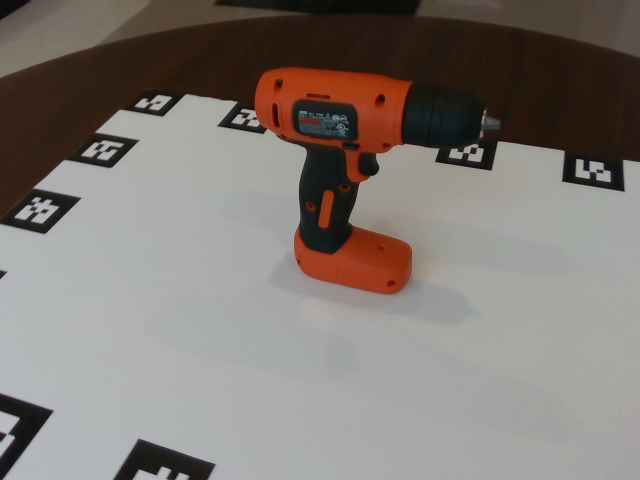
\includegraphics[width=\ew cm,height=\eh cm]{assets/images/appendix/objects/sos_rgb49.jpg}};
\node[anchor=north west,inner sep=0pt] at (0.36,-2.08) {
\includegraphics[width=\ew cm,height=\eh cm]{assets/images/appendix/objects/sos_mask49.png}};
\draw[rpxAccent,line width=.35pt] (0.36,0) rectangle ++(\ew,-\eh); \draw[rpxAccent,line width=.35pt] (0.36,-2.08) rectangle ++(\ew,-\eh);
\node[anchor=north,inner sep=0pt,font=\fontsize{7.5}{9}\selectfont] at (1.68,-4.16) {49\enspace power drill};
\node[anchor=north west,inner sep=0pt] at (3.10,0) {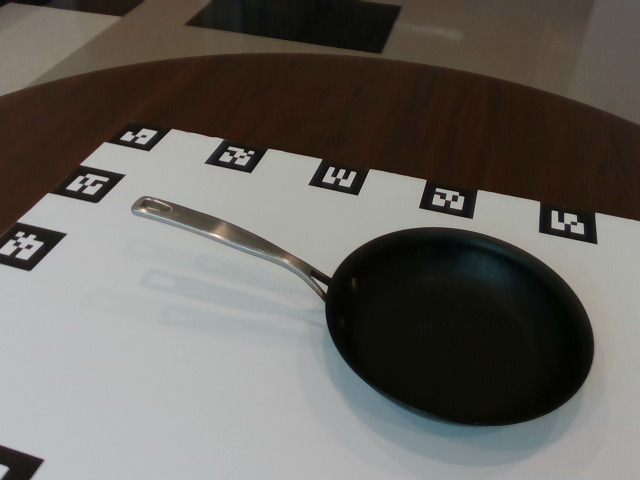
\includegraphics[width=\ew cm,height=\eh cm]{assets/images/appendix/objects/sos_rgb21.jpg}};
\node[anchor=north west,inner sep=0pt] at (3.10,-2.08) {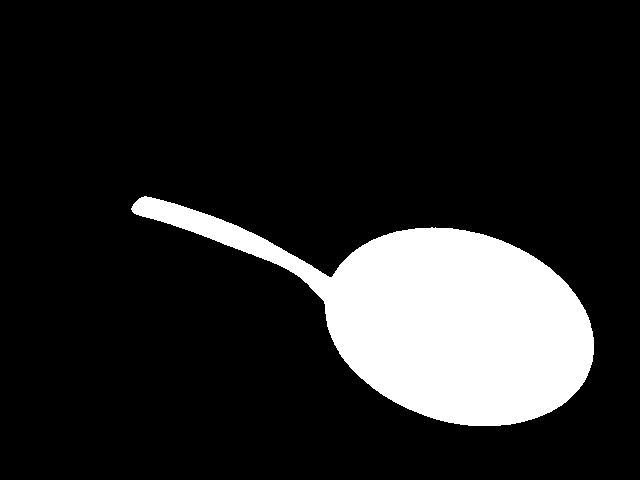
\includegraphics[width=\ew cm,height=\eh cm]{assets/images/appendix/objects/sos_mask21.png}};
\draw[rpxAccent,line width=.35pt] (3.10,0) rectangle ++(\ew,-\eh); \draw[rpxAccent,line width=.35pt] (3.10,-2.08) rectangle ++(\ew,-\eh);
\node[anchor=north,inner sep=0pt,font=\fontsize{7.5}{9}\selectfont] at (4.42,-4.16) {21\enspace fry pan};
\node[anchor=north west,inner sep=0pt] at (5.84,0) {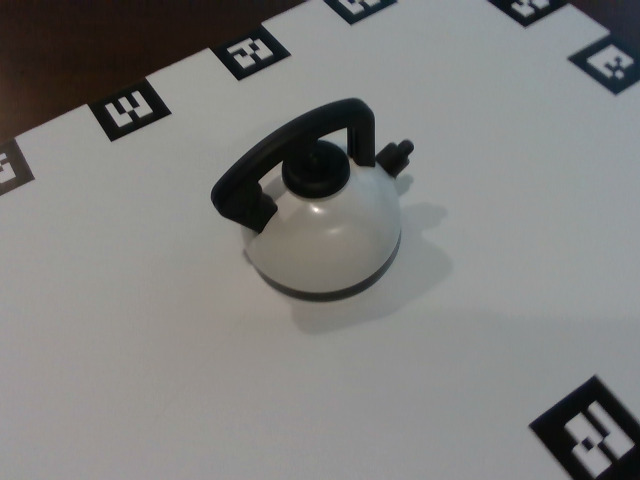
\includegraphics[width=\ew cm,height=\eh cm]{assets/images/appendix/objects/sos_rgb65.jpg}};
\node[anchor=north west,inner sep=0pt] at (5.84,-2.08) {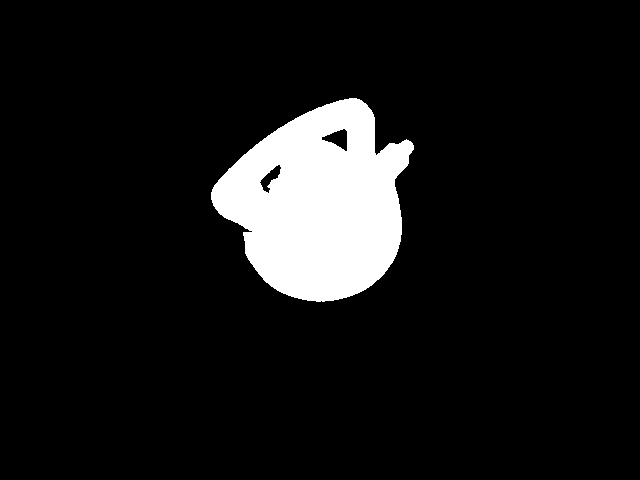
\includegraphics[width=\ew cm,height=\eh cm]{assets/images/appendix/objects/sos_mask65.png}};
\draw[rpxAccent,line width=.35pt] (5.84,0) rectangle ++(\ew,-\eh); \draw[rpxAccent,line width=.35pt] (5.84,-2.08) rectangle ++(\ew,-\eh);
\node[anchor=north,inner sep=0pt,font=\fontsize{7.5}{9}\selectfont] at (7.16,-4.16) {65\enspace teapot};
\node[anchor=east,inner sep=0pt,font=\fontsize{7.5}{9}\selectfont,text=rpxSlate,rotate=90] at (0.24,-0.99) {RGB};
\node[anchor=east,inner sep=0pt,font=\fontsize{7.5}{9}\selectfont,text=rpxSlate,rotate=90] at (0.24,-3.07) {mask};
\end{tikzpicture}

\captionof{figure}{SOS capture examples: released RGB frames (top) and their instance masks (bottom).}
\label{fig:sos-examples}
\end{minipage}\par\medskip

\begin{figure*}[p]
\centering
% Generated by tools/web_assets/build_web_assets.py -- all 70 SOS objects, segmented with
% their released instance masks, numbered as in the canonical catalogue.
\begin{tikzpicture}[x=1cm,y=1cm]
\def\ow{1.88}\def\og{0.1}\def\ol{0.62}
\node[anchor=north west,inner sep=0pt] at (0.000,0.000) {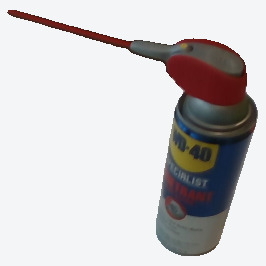
\includegraphics[width=\ow cm,height=\ow cm]{assets/images/appendix/objects/obj01.jpg}};
\node[anchor=north west,inner sep=0pt,text width=\ow cm,align=left,font=\fontsize{7.5}{8.6}\selectfont] at (0.000,-1.950) {\textbf{1}\enspace air duster can};
\node[anchor=north west,inner sep=0pt] at (1.980,0.000) {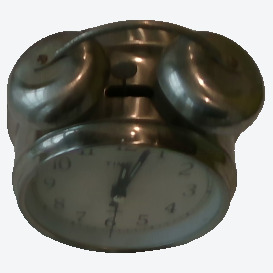
\includegraphics[width=\ow cm,height=\ow cm]{assets/images/appendix/objects/obj02.jpg}};
\node[anchor=north west,inner sep=0pt,text width=\ow cm,align=left,font=\fontsize{7.5}{8.6}\selectfont] at (1.980,-1.950) {\textbf{2}\enspace alarm clock};
\node[anchor=north west,inner sep=0pt] at (3.960,0.000) {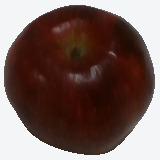
\includegraphics[width=\ow cm,height=\ow cm]{assets/images/appendix/objects/obj03.jpg}};
\node[anchor=north west,inner sep=0pt,text width=\ow cm,align=left,font=\fontsize{7.5}{8.6}\selectfont] at (3.960,-1.950) {\textbf{3}\enspace apple};
\node[anchor=north west,inner sep=0pt] at (5.940,0.000) {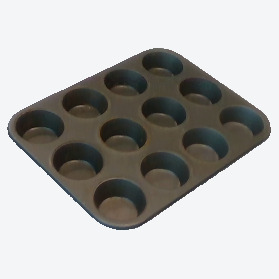
\includegraphics[width=\ow cm,height=\ow cm]{assets/images/appendix/objects/obj04.jpg}};
\node[anchor=north west,inner sep=0pt,text width=\ow cm,align=left,font=\fontsize{7.5}{8.6}\selectfont] at (5.940,-1.950) {\textbf{4}\enspace baking tray};
\node[anchor=north west,inner sep=0pt] at (7.920,0.000) {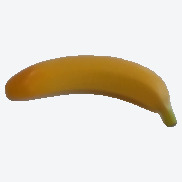
\includegraphics[width=\ow cm,height=\ow cm]{assets/images/appendix/objects/obj05.jpg}};
\node[anchor=north west,inner sep=0pt,text width=\ow cm,align=left,font=\fontsize{7.5}{8.6}\selectfont] at (7.920,-1.950) {\textbf{5}\enspace banana};
\node[anchor=north west,inner sep=0pt] at (9.900,0.000) {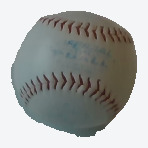
\includegraphics[width=\ow cm,height=\ow cm]{assets/images/appendix/objects/obj06.jpg}};
\node[anchor=north west,inner sep=0pt,text width=\ow cm,align=left,font=\fontsize{7.5}{8.6}\selectfont] at (9.900,-1.950) {\textbf{6}\enspace baseball ball};
\node[anchor=north west,inner sep=0pt] at (11.880,0.000) {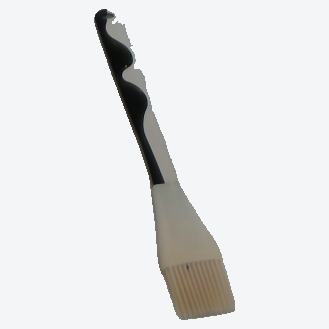
\includegraphics[width=\ow cm,height=\ow cm]{assets/images/appendix/objects/obj07.jpg}};
\node[anchor=north west,inner sep=0pt,text width=\ow cm,align=left,font=\fontsize{7.5}{8.6}\selectfont] at (11.880,-1.950) {\textbf{7}\enspace basting brush};
\node[anchor=north west,inner sep=0pt] at (13.860,0.000) {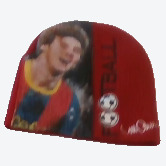
\includegraphics[width=\ow cm,height=\ow cm]{assets/images/appendix/objects/obj08.jpg}};
\node[anchor=north west,inner sep=0pt,text width=\ow cm,align=left,font=\fontsize{7.5}{8.6}\selectfont] at (13.860,-1.950) {\textbf{8}\enspace beanie};
\node[anchor=north west,inner sep=0pt] at (15.840,0.000) {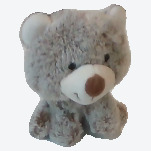
\includegraphics[width=\ow cm,height=\ow cm]{assets/images/appendix/objects/obj09.jpg}};
\node[anchor=north west,inner sep=0pt,text width=\ow cm,align=left,font=\fontsize{7.5}{8.6}\selectfont] at (15.840,-1.950) {\textbf{9}\enspace bear};
\node[anchor=north west,inner sep=0pt] at (0.000,-2.500) {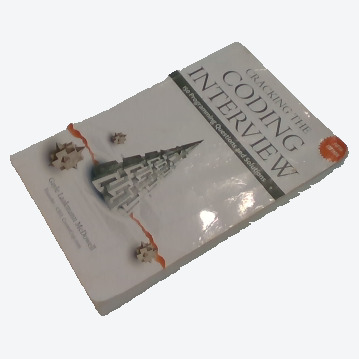
\includegraphics[width=\ow cm,height=\ow cm]{assets/images/appendix/objects/obj10.jpg}};
\node[anchor=north west,inner sep=0pt,text width=\ow cm,align=left,font=\fontsize{7.5}{8.6}\selectfont] at (0.000,-4.450) {\textbf{10}\enspace book};
\node[anchor=north west,inner sep=0pt] at (1.980,-2.500) {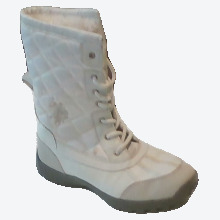
\includegraphics[width=\ow cm,height=\ow cm]{assets/images/appendix/objects/obj11.jpg}};
\node[anchor=north west,inner sep=0pt,text width=\ow cm,align=left,font=\fontsize{7.5}{8.6}\selectfont] at (1.980,-4.450) {\textbf{11}\enspace boot};
\node[anchor=north west,inner sep=0pt] at (3.960,-2.500) {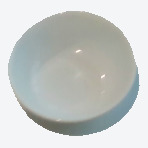
\includegraphics[width=\ow cm,height=\ow cm]{assets/images/appendix/objects/obj12.jpg}};
\node[anchor=north west,inner sep=0pt,text width=\ow cm,align=left,font=\fontsize{7.5}{8.6}\selectfont] at (3.960,-4.450) {\textbf{12}\enspace bowl};
\node[anchor=north west,inner sep=0pt] at (5.940,-2.500) {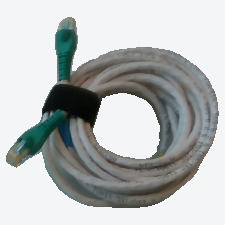
\includegraphics[width=\ow cm,height=\ow cm]{assets/images/appendix/objects/obj13.jpg}};
\node[anchor=north west,inner sep=0pt,text width=\ow cm,align=left,font=\fontsize{7.5}{8.6}\selectfont] at (5.940,-4.450) {\textbf{13}\enspace cable};
\node[anchor=north west,inner sep=0pt] at (7.920,-2.500) {
\includegraphics[width=\ow cm,height=\ow cm]{assets/images/appendix/objects/obj14.jpg}};
\node[anchor=north west,inner sep=0pt,text width=\ow cm,align=left,font=\fontsize{7.5}{8.6}\selectfont] at (7.920,-4.450) {\textbf{14}\enspace candy bar};
\node[anchor=north west,inner sep=0pt] at (9.900,-2.500) {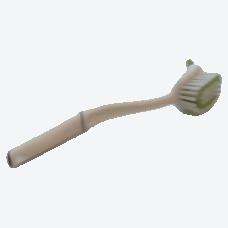
\includegraphics[width=\ow cm,height=\ow cm]{assets/images/appendix/objects/obj15.jpg}};
\node[anchor=north west,inner sep=0pt,text width=\ow cm,align=left,font=\fontsize{7.5}{8.6}\selectfont] at (9.900,-4.450) {\textbf{15}\enspace cleaning brush};
\node[anchor=north west,inner sep=0pt] at (11.880,-2.500) {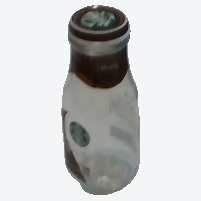
\includegraphics[width=\ow cm,height=\ow cm]{assets/images/appendix/objects/obj16.jpg}};
\node[anchor=north west,inner sep=0pt,text width=\ow cm,align=left,font=\fontsize{7.5}{8.6}\selectfont] at (11.880,-4.450) {\textbf{16}\enspace coffee bottle};
\node[anchor=north west,inner sep=0pt] at (13.860,-2.500) {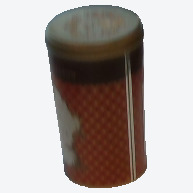
\includegraphics[width=\ow cm,height=\ow cm]{assets/images/appendix/objects/obj17.jpg}};
\node[anchor=north west,inner sep=0pt,text width=\ow cm,align=left,font=\fontsize{7.5}{8.6}\selectfont] at (13.860,-4.450) {\textbf{17}\enspace coffee can};
\node[anchor=north west,inner sep=0pt] at (15.840,-2.500) {
\includegraphics[width=\ow cm,height=\ow cm]{assets/images/appendix/objects/obj18.jpg}};
\node[anchor=north west,inner sep=0pt,text width=\ow cm,align=left,font=\fontsize{7.5}{8.6}\selectfont] at (15.840,-4.450) {\textbf{18}\enspace cracker box};
\node[anchor=north west,inner sep=0pt] at (0.000,-5.000) {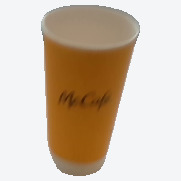
\includegraphics[width=\ow cm,height=\ow cm]{assets/images/appendix/objects/obj19.jpg}};
\node[anchor=north west,inner sep=0pt,text width=\ow cm,align=left,font=\fontsize{7.5}{8.6}\selectfont] at (0.000,-6.950) {\textbf{19}\enspace cup};
\node[anchor=north west,inner sep=0pt] at (1.980,-5.000) {
\includegraphics[width=\ow cm,height=\ow cm]{assets/images/appendix/objects/obj20.jpg}};
\node[anchor=north west,inner sep=0pt,text width=\ow cm,align=left,font=\fontsize{7.5}{8.6}\selectfont] at (1.980,-6.950) {\textbf{20}\enspace doll};
\node[anchor=north west,inner sep=0pt] at (3.960,-5.000) {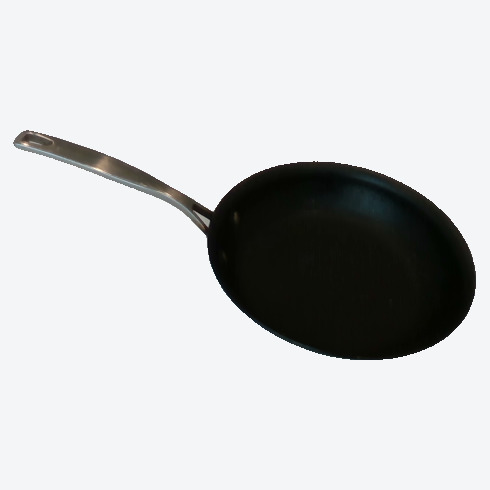
\includegraphics[width=\ow cm,height=\ow cm]{assets/images/appendix/objects/obj21.jpg}};
\node[anchor=north west,inner sep=0pt,text width=\ow cm,align=left,font=\fontsize{7.5}{8.6}\selectfont] at (3.960,-6.950) {\textbf{21}\enspace fry pan};
\node[anchor=north west,inner sep=0pt] at (5.940,-5.000) {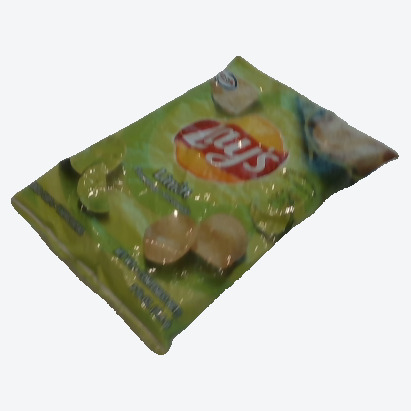
\includegraphics[width=\ow cm,height=\ow cm]{assets/images/appendix/objects/obj22.jpg}};
\node[anchor=north west,inner sep=0pt,text width=\ow cm,align=left,font=\fontsize{7.5}{8.6}\selectfont] at (5.940,-6.950) {\textbf{22}\enspace food bag};
\node[anchor=north west,inner sep=0pt] at (7.920,-5.000) {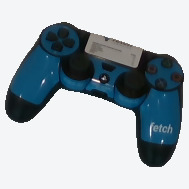
\includegraphics[width=\ow cm,height=\ow cm]{assets/images/appendix/objects/obj23.jpg}};
\node[anchor=north west,inner sep=0pt,text width=\ow cm,align=left,font=\fontsize{7.5}{8.6}\selectfont] at (7.920,-6.950) {\textbf{23}\enspace game controller};
\node[anchor=north west,inner sep=0pt] at (9.900,-5.000) {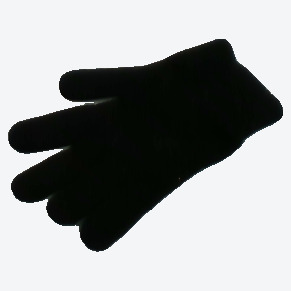
\includegraphics[width=\ow cm,height=\ow cm]{assets/images/appendix/objects/obj24.jpg}};
\node[anchor=north west,inner sep=0pt,text width=\ow cm,align=left,font=\fontsize{7.5}{8.6}\selectfont] at (9.900,-6.950) {\textbf{24}\enspace glove};
\node[anchor=north west,inner sep=0pt] at (11.880,-5.000) {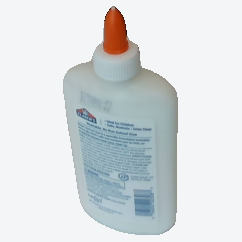
\includegraphics[width=\ow cm,height=\ow cm]{assets/images/appendix/objects/obj25.jpg}};
\node[anchor=north west,inner sep=0pt,text width=\ow cm,align=left,font=\fontsize{7.5}{8.6}\selectfont] at (11.880,-6.950) {\textbf{25}\enspace glue bottle};
\node[anchor=north west,inner sep=0pt] at (13.860,-5.000) {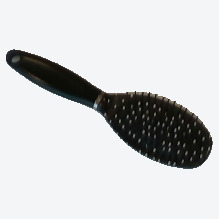
\includegraphics[width=\ow cm,height=\ow cm]{assets/images/appendix/objects/obj26.jpg}};
\node[anchor=north west,inner sep=0pt,text width=\ow cm,align=left,font=\fontsize{7.5}{8.6}\selectfont] at (13.860,-6.950) {\textbf{26}\enspace hair brush};
\node[anchor=north west,inner sep=0pt] at (15.840,-5.000) {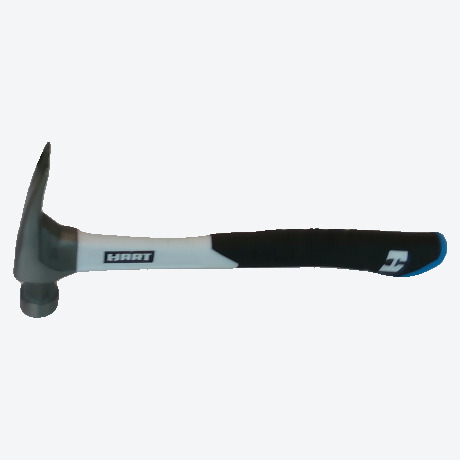
\includegraphics[width=\ow cm,height=\ow cm]{assets/images/appendix/objects/obj27.jpg}};
\node[anchor=north west,inner sep=0pt,text width=\ow cm,align=left,font=\fontsize{7.5}{8.6}\selectfont] at (15.840,-6.950) {\textbf{27}\enspace hammer};
\node[anchor=north west,inner sep=0pt] at (0.000,-7.500) {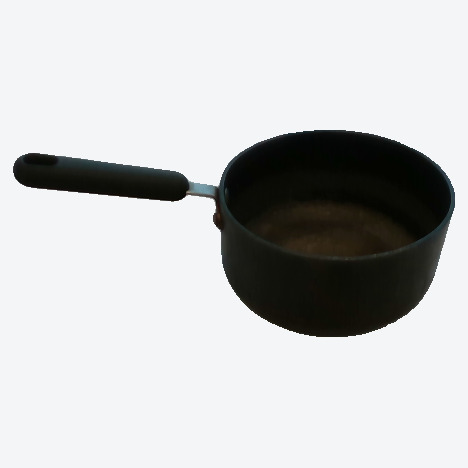
\includegraphics[width=\ow cm,height=\ow cm]{assets/images/appendix/objects/obj28.jpg}};
\node[anchor=north west,inner sep=0pt,text width=\ow cm,align=left,font=\fontsize{7.5}{8.6}\selectfont] at (0.000,-9.450) {\textbf{28}\enspace handy pot};
\node[anchor=north west,inner sep=0pt] at (1.980,-7.500) {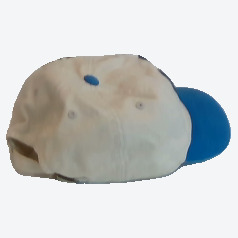
\includegraphics[width=\ow cm,height=\ow cm]{assets/images/appendix/objects/obj29.jpg}};
\node[anchor=north west,inner sep=0pt,text width=\ow cm,align=left,font=\fontsize{7.5}{8.6}\selectfont] at (1.980,-9.450) {\textbf{29}\enspace hat};
\node[anchor=north west,inner sep=0pt] at (3.960,-7.500) {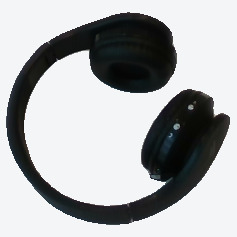
\includegraphics[width=\ow cm,height=\ow cm]{assets/images/appendix/objects/obj30.jpg}};
\node[anchor=north west,inner sep=0pt,text width=\ow cm,align=left,font=\fontsize{7.5}{8.6}\selectfont] at (3.960,-9.450) {\textbf{30}\enspace headphone};
\node[anchor=north west,inner sep=0pt] at (5.940,-7.500) {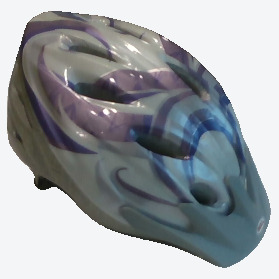
\includegraphics[width=\ow cm,height=\ow cm]{assets/images/appendix/objects/obj31.jpg}};
\node[anchor=north west,inner sep=0pt,text width=\ow cm,align=left,font=\fontsize{7.5}{8.6}\selectfont] at (5.940,-9.450) {\textbf{31}\enspace helmet};
\node[anchor=north west,inner sep=0pt] at (7.920,-7.500) {
\includegraphics[width=\ow cm,height=\ow cm]{assets/images/appendix/objects/obj32.jpg}};
\node[anchor=north west,inner sep=0pt,text width=\ow cm,align=left,font=\fontsize{7.5}{8.6}\selectfont] at (7.920,-9.450) {\textbf{32}\enspace instant noodle packet};
\node[anchor=north west,inner sep=0pt] at (9.900,-7.500) {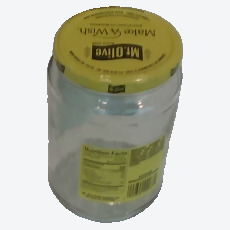
\includegraphics[width=\ow cm,height=\ow cm]{assets/images/appendix/objects/obj33.jpg}};
\node[anchor=north west,inner sep=0pt,text width=\ow cm,align=left,font=\fontsize{7.5}{8.6}\selectfont] at (9.900,-9.450) {\textbf{33}\enspace jar};
\node[anchor=north west,inner sep=0pt] at (11.880,-7.500) {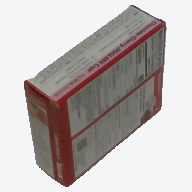
\includegraphics[width=\ow cm,height=\ow cm]{assets/images/appendix/objects/obj34.jpg}};
\node[anchor=north west,inner sep=0pt,text width=\ow cm,align=left,font=\fontsize{7.5}{8.6}\selectfont] at (11.880,-9.450) {\textbf{34}\enspace jello box};
\node[anchor=north west,inner sep=0pt] at (13.860,-7.500) {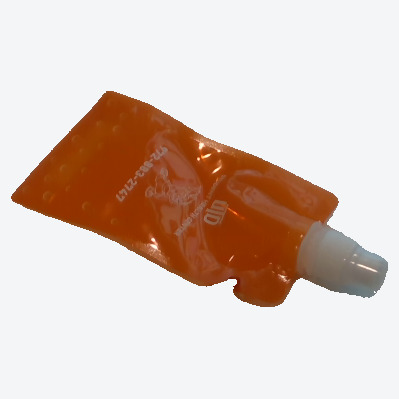
\includegraphics[width=\ow cm,height=\ow cm]{assets/images/appendix/objects/obj35.jpg}};
\node[anchor=north west,inner sep=0pt,text width=\ow cm,align=left,font=\fontsize{7.5}{8.6}\selectfont] at (13.860,-9.450) {\textbf{35}\enspace juice pouch};
\node[anchor=north west,inner sep=0pt] at (15.840,-7.500) {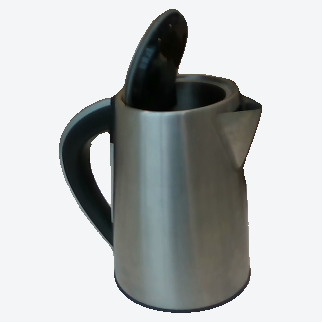
\includegraphics[width=\ow cm,height=\ow cm]{assets/images/appendix/objects/obj36.jpg}};
\node[anchor=north west,inner sep=0pt,text width=\ow cm,align=left,font=\fontsize{7.5}{8.6}\selectfont] at (15.840,-9.450) {\textbf{36}\enspace kettle};
\node[anchor=north west,inner sep=0pt] at (0.000,-10.000) {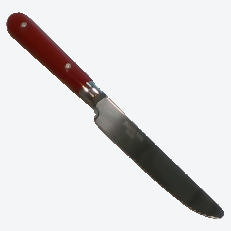
\includegraphics[width=\ow cm,height=\ow cm]{assets/images/appendix/objects/obj37.jpg}};
\node[anchor=north west,inner sep=0pt,text width=\ow cm,align=left,font=\fontsize{7.5}{8.6}\selectfont] at (0.000,-11.950) {\textbf{37}\enspace knife};
\node[anchor=north west,inner sep=0pt] at (1.980,-10.000) {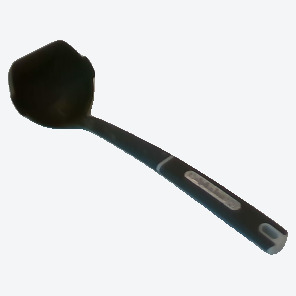
\includegraphics[width=\ow cm,height=\ow cm]{assets/images/appendix/objects/obj38.jpg}};
\node[anchor=north west,inner sep=0pt,text width=\ow cm,align=left,font=\fontsize{7.5}{8.6}\selectfont] at (1.980,-11.950) {\textbf{38}\enspace ladle};
\node[anchor=north west,inner sep=0pt] at (3.960,-10.000) {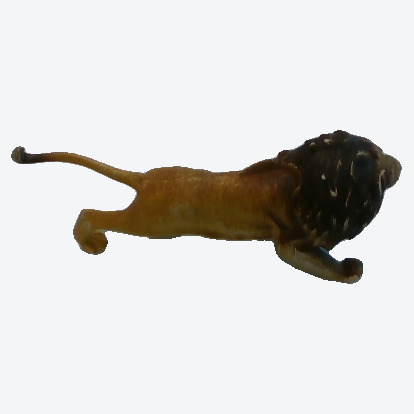
\includegraphics[width=\ow cm,height=\ow cm]{assets/images/appendix/objects/obj39.jpg}};
\node[anchor=north west,inner sep=0pt,text width=\ow cm,align=left,font=\fontsize{7.5}{8.6}\selectfont] at (3.960,-11.950) {\textbf{39}\enspace lion};
\node[anchor=north west,inner sep=0pt] at (5.940,-10.000) {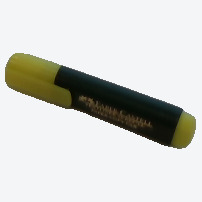
\includegraphics[width=\ow cm,height=\ow cm]{assets/images/appendix/objects/obj40.jpg}};
\node[anchor=north west,inner sep=0pt,text width=\ow cm,align=left,font=\fontsize{7.5}{8.6}\selectfont] at (5.940,-11.950) {\textbf{40}\enspace marker};
\node[anchor=north west,inner sep=0pt] at (7.920,-10.000) {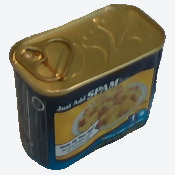
\includegraphics[width=\ow cm,height=\ow cm]{assets/images/appendix/objects/obj41.jpg}};
\node[anchor=north west,inner sep=0pt,text width=\ow cm,align=left,font=\fontsize{7.5}{8.6}\selectfont] at (7.920,-11.950) {\textbf{41}\enspace meat can};
\node[anchor=north west,inner sep=0pt] at (9.900,-10.000) {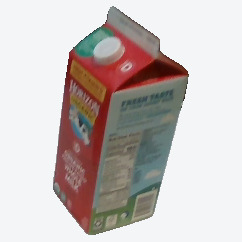
\includegraphics[width=\ow cm,height=\ow cm]{assets/images/appendix/objects/obj42.jpg}};
\node[anchor=north west,inner sep=0pt,text width=\ow cm,align=left,font=\fontsize{7.5}{8.6}\selectfont] at (9.900,-11.950) {\textbf{42}\enspace milk box};
\node[anchor=north west,inner sep=0pt] at (11.880,-10.000) {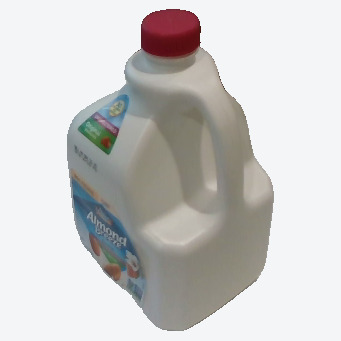
\includegraphics[width=\ow cm,height=\ow cm]{assets/images/appendix/objects/obj43.jpg}};
\node[anchor=north west,inner sep=0pt,text width=\ow cm,align=left,font=\fontsize{7.5}{8.6}\selectfont] at (11.880,-11.950) {\textbf{43}\enspace milk jug};
\node[anchor=north west,inner sep=0pt] at (13.860,-10.000) {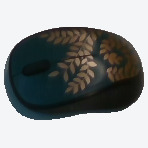
\includegraphics[width=\ow cm,height=\ow cm]{assets/images/appendix/objects/obj44.jpg}};
\node[anchor=north west,inner sep=0pt,text width=\ow cm,align=left,font=\fontsize{7.5}{8.6}\selectfont] at (13.860,-11.950) {\textbf{44}\enspace mouse};
\node[anchor=north west,inner sep=0pt] at (15.840,-10.000) {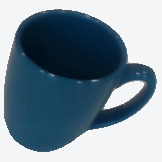
\includegraphics[width=\ow cm,height=\ow cm]{assets/images/appendix/objects/obj45.jpg}};
\node[anchor=north west,inner sep=0pt,text width=\ow cm,align=left,font=\fontsize{7.5}{8.6}\selectfont] at (15.840,-11.950) {\textbf{45}\enspace mug};
\node[anchor=north west,inner sep=0pt] at (0.000,-12.500) {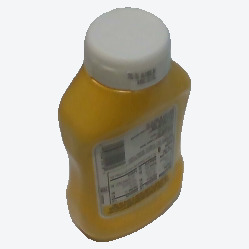
\includegraphics[width=\ow cm,height=\ow cm]{assets/images/appendix/objects/obj46.jpg}};
\node[anchor=north west,inner sep=0pt,text width=\ow cm,align=left,font=\fontsize{7.5}{8.6}\selectfont] at (0.000,-14.450) {\textbf{46}\enspace mustard bottle};
\node[anchor=north west,inner sep=0pt] at (1.980,-12.500) {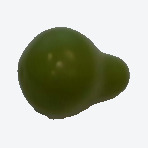
\includegraphics[width=\ow cm,height=\ow cm]{assets/images/appendix/objects/obj47.jpg}};
\node[anchor=north west,inner sep=0pt,text width=\ow cm,align=left,font=\fontsize{7.5}{8.6}\selectfont] at (1.980,-14.450) {\textbf{47}\enspace pear};
\node[anchor=north west,inner sep=0pt] at (3.960,-12.500) {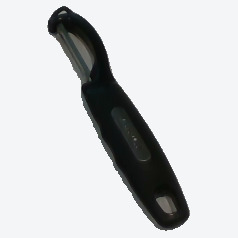
\includegraphics[width=\ow cm,height=\ow cm]{assets/images/appendix/objects/obj48.jpg}};
\node[anchor=north west,inner sep=0pt,text width=\ow cm,align=left,font=\fontsize{7.5}{8.6}\selectfont] at (3.960,-14.450) {\textbf{48}\enspace peeler};
\node[anchor=north west,inner sep=0pt] at (5.940,-12.500) {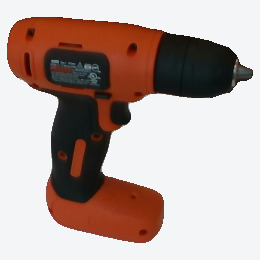
\includegraphics[width=\ow cm,height=\ow cm]{assets/images/appendix/objects/obj49.jpg}};
\node[anchor=north west,inner sep=0pt,text width=\ow cm,align=left,font=\fontsize{7.5}{8.6}\selectfont] at (5.940,-14.450) {\textbf{49}\enspace power drill};
\node[anchor=north west,inner sep=0pt] at (7.920,-12.500) {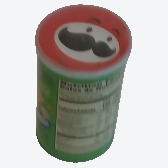
\includegraphics[width=\ow cm,height=\ow cm]{assets/images/appendix/objects/obj50.jpg}};
\node[anchor=north west,inner sep=0pt,text width=\ow cm,align=left,font=\fontsize{7.5}{8.6}\selectfont] at (7.920,-14.450) {\textbf{50}\enspace pringles can};
\node[anchor=north west,inner sep=0pt] at (9.900,-12.500) {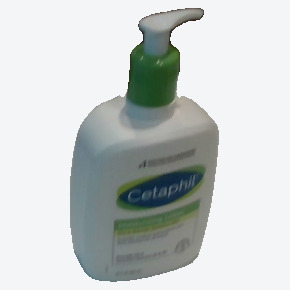
\includegraphics[width=\ow cm,height=\ow cm]{assets/images/appendix/objects/obj51.jpg}};
\node[anchor=north west,inner sep=0pt,text width=\ow cm,align=left,font=\fontsize{7.5}{8.6}\selectfont] at (9.900,-14.450) {\textbf{51}\enspace pump bottle};
\node[anchor=north west,inner sep=0pt] at (11.880,-12.500) {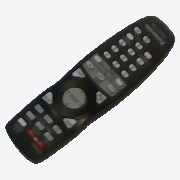
\includegraphics[width=\ow cm,height=\ow cm]{assets/images/appendix/objects/obj52.jpg}};
\node[anchor=north west,inner sep=0pt,text width=\ow cm,align=left,font=\fontsize{7.5}{8.6}\selectfont] at (11.880,-14.450) {\textbf{52}\enspace remote controller};
\node[anchor=north west,inner sep=0pt] at (13.860,-12.500) {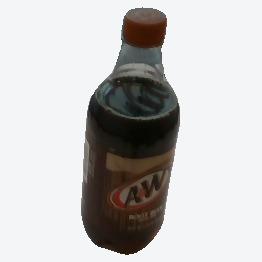
\includegraphics[width=\ow cm,height=\ow cm]{assets/images/appendix/objects/obj53.jpg}};
\node[anchor=north west,inner sep=0pt,text width=\ow cm,align=left,font=\fontsize{7.5}{8.6}\selectfont] at (13.860,-14.450) {\textbf{53}\enspace root beer bottle};
\node[anchor=north west,inner sep=0pt] at (15.840,-12.500) {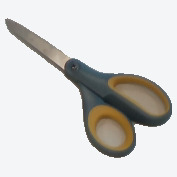
\includegraphics[width=\ow cm,height=\ow cm]{assets/images/appendix/objects/obj54.jpg}};
\node[anchor=north west,inner sep=0pt,text width=\ow cm,align=left,font=\fontsize{7.5}{8.6}\selectfont] at (15.840,-14.450) {\textbf{54}\enspace scissors};
\node[anchor=north west,inner sep=0pt] at (0.000,-15.000) {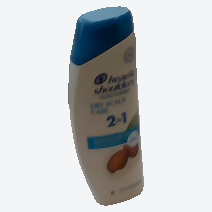
\includegraphics[width=\ow cm,height=\ow cm]{assets/images/appendix/objects/obj55.jpg}};
\node[anchor=north west,inner sep=0pt,text width=\ow cm,align=left,font=\fontsize{7.5}{8.6}\selectfont] at (0.000,-16.950) {\textbf{55}\enspace shampoo bottle};
\node[anchor=north west,inner sep=0pt] at (1.980,-15.000) {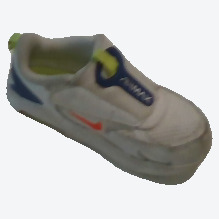
\includegraphics[width=\ow cm,height=\ow cm]{assets/images/appendix/objects/obj56.jpg}};
\node[anchor=north west,inner sep=0pt,text width=\ow cm,align=left,font=\fontsize{7.5}{8.6}\selectfont] at (1.980,-16.950) {\textbf{56}\enspace shoe};
\node[anchor=north west,inner sep=0pt] at (3.960,-15.000) {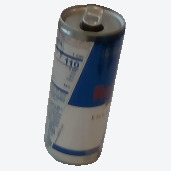
\includegraphics[width=\ow cm,height=\ow cm]{assets/images/appendix/objects/obj57.jpg}};
\node[anchor=north west,inner sep=0pt,text width=\ow cm,align=left,font=\fontsize{7.5}{8.6}\selectfont] at (3.960,-16.950) {\textbf{57}\enspace soda can};
\node[anchor=north west,inner sep=0pt] at (5.940,-15.000) {
\includegraphics[width=\ow cm,height=\ow cm]{assets/images/appendix/objects/obj58.jpg}};
\node[anchor=north west,inner sep=0pt,text width=\ow cm,align=left,font=\fontsize{7.5}{8.6}\selectfont] at (5.940,-16.950) {\textbf{58}\enspace soft scrub cleanser bottle};
\node[anchor=north west,inner sep=0pt] at (7.920,-15.000) {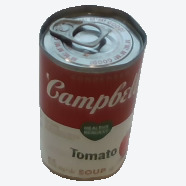
\includegraphics[width=\ow cm,height=\ow cm]{assets/images/appendix/objects/obj59.jpg}};
\node[anchor=north west,inner sep=0pt,text width=\ow cm,align=left,font=\fontsize{7.5}{8.6}\selectfont] at (7.920,-16.950) {\textbf{59}\enspace soup can};
\node[anchor=north west,inner sep=0pt] at (9.900,-15.000) {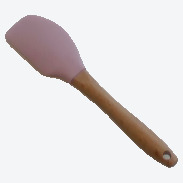
\includegraphics[width=\ow cm,height=\ow cm]{assets/images/appendix/objects/obj60.jpg}};
\node[anchor=north west,inner sep=0pt,text width=\ow cm,align=left,font=\fontsize{7.5}{8.6}\selectfont] at (9.900,-16.950) {\textbf{60}\enspace spatula};
\node[anchor=north west,inner sep=0pt] at (11.880,-15.000) {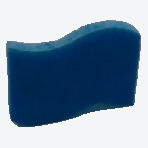
\includegraphics[width=\ow cm,height=\ow cm]{assets/images/appendix/objects/obj61.jpg}};
\node[anchor=north west,inner sep=0pt,text width=\ow cm,align=left,font=\fontsize{7.5}{8.6}\selectfont] at (11.880,-16.950) {\textbf{61}\enspace sponge};
\node[anchor=north west,inner sep=0pt] at (13.860,-15.000) {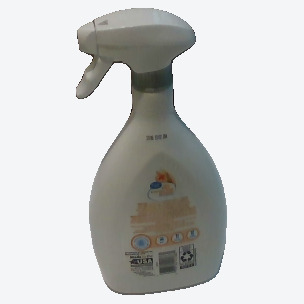
\includegraphics[width=\ow cm,height=\ow cm]{assets/images/appendix/objects/obj62.jpg}};
\node[anchor=north west,inner sep=0pt,text width=\ow cm,align=left,font=\fontsize{7.5}{8.6}\selectfont] at (13.860,-16.950) {\textbf{62}\enspace spray bottle};
\node[anchor=north west,inner sep=0pt] at (15.840,-15.000) {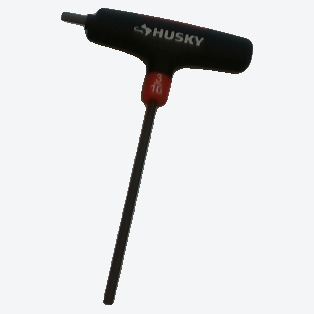
\includegraphics[width=\ow cm,height=\ow cm]{assets/images/appendix/objects/obj63.jpg}};
\node[anchor=north west,inner sep=0pt,text width=\ow cm,align=left,font=\fontsize{7.5}{8.6}\selectfont] at (15.840,-16.950) {\textbf{63}\enspace t-handle};
\node[anchor=north west,inner sep=0pt] at (0.000,-17.500) {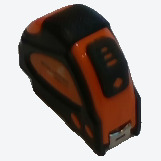
\includegraphics[width=\ow cm,height=\ow cm]{assets/images/appendix/objects/obj64.jpg}};
\node[anchor=north west,inner sep=0pt,text width=\ow cm,align=left,font=\fontsize{7.5}{8.6}\selectfont] at (0.000,-19.450) {\textbf{64}\enspace tape measure};
\node[anchor=north west,inner sep=0pt] at (1.980,-17.500) {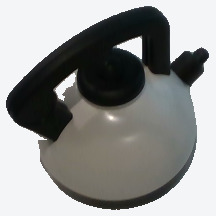
\includegraphics[width=\ow cm,height=\ow cm]{assets/images/appendix/objects/obj65.jpg}};
\node[anchor=north west,inner sep=0pt,text width=\ow cm,align=left,font=\fontsize{7.5}{8.6}\selectfont] at (1.980,-19.450) {\textbf{65}\enspace teapot};
\node[anchor=north west,inner sep=0pt] at (3.960,-17.500) {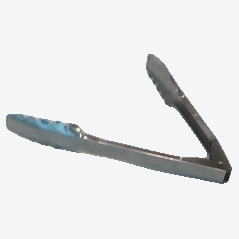
\includegraphics[width=\ow cm,height=\ow cm]{assets/images/appendix/objects/obj66.jpg}};
\node[anchor=north west,inner sep=0pt,text width=\ow cm,align=left,font=\fontsize{7.5}{8.6}\selectfont] at (3.960,-19.450) {\textbf{66}\enspace tong};
\node[anchor=north west,inner sep=0pt] at (5.940,-17.500) {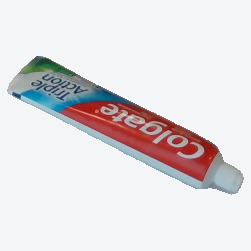
\includegraphics[width=\ow cm,height=\ow cm]{assets/images/appendix/objects/obj67.jpg}};
\node[anchor=north west,inner sep=0pt,text width=\ow cm,align=left,font=\fontsize{7.5}{8.6}\selectfont] at (5.940,-19.450) {\textbf{67}\enspace toothpaste};
\node[anchor=north west,inner sep=0pt] at (7.920,-17.500) {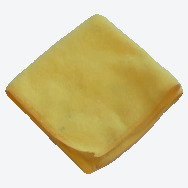
\includegraphics[width=\ow cm,height=\ow cm]{assets/images/appendix/objects/obj68.jpg}};
\node[anchor=north west,inner sep=0pt,text width=\ow cm,align=left,font=\fontsize{7.5}{8.6}\selectfont] at (7.920,-19.450) {\textbf{68}\enspace towel};
\node[anchor=north west,inner sep=0pt] at (9.900,-17.500) {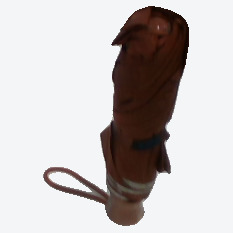
\includegraphics[width=\ow cm,height=\ow cm]{assets/images/appendix/objects/obj69.jpg}};
\node[anchor=north west,inner sep=0pt,text width=\ow cm,align=left,font=\fontsize{7.5}{8.6}\selectfont] at (9.900,-19.450) {\textbf{69}\enspace umbrella};
\node[anchor=north west,inner sep=0pt] at (11.880,-17.500) {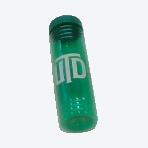
\includegraphics[width=\ow cm,height=\ow cm]{assets/images/appendix/objects/obj70.jpg}};
\node[anchor=north west,inner sep=0pt,text width=\ow cm,align=left,font=\fontsize{7.5}{8.6}\selectfont] at (11.880,-19.450) {\textbf{70}\enspace water bottle};
\end{tikzpicture}

\caption{All 70 SOS objects, each cut out of one released SOS frame with its instance mask and numbered as in Table~\ref{tab:sos-canonical}.}
\label{fig:sos-gallery}
\end{figure*}

\subsection{Questionnaire schema}

Each object has a stable \texttt{object\_id}, a contiguous \texttt{global\_object\_id}, and multiple human responses (Table~\ref{tab:sos-schema}). These responses generate regular attribute questions and supply identity references for in-context VQA. Table~\ref{tab:sos-canonical} reports one lightly normalized canonical response per field for readability; the benchmark release preserves the original annotator responses, aliases, and attribute variants.

\par\medskip\noindent\begin{minipage}{\columnwidth}
\centering
\captionof{table}{SOS questionnaire schema.}
\label{tab:sos-schema}
\footnotesize
\setlength{\tabcolsep}{0pt}
\begin{tabular*}{\columnwidth}{@{}l@{\extracolsep{\fill}}ll@{}}
\toprule
Field & Meaning / prompt & Benchmark use \\
\midrule
Name & Names and valid aliases & Direct reference \\
Category & Semantic object class & Attribute reference \\
Colour & Visible colour descriptions & Attribute reference \\
Material & Constituent material & Attribute reference \\
Function & Common purpose or action & Functional reference \\
\bottomrule
\end{tabular*}
\end{minipage}\par\medskip

\subsection{Canonical catalogue}

Table~\ref{tab:sos-canonical} lists all 70 objects with their canonical responses.

% Table XIII -- canonical SOS questionnaire catalogue (all 70 objects), set as
% four column blocks balanced over the last two pages; each continuation block
% repeats the table number and the column heads.
\begingroup
\fontsize{\catfs}{\catlead}\selectfont
\setlength{\tabcolsep}{3pt}\renewcommand{\arraystretch}{1}
\noindent\begin{minipage}[t]{\columnwidth}\centering
{\normalsize\captionof{table}{Canonical SOS questionnaire catalogue. Each entry lists the object name and one lightly normalized canonical category, colour, material, and function response.}\label{tab:sos-canonical}}
\begin{tabular}{@{}>{\bfseries}r@{\hspace{5pt}}>{\raggedright\arraybackslash}p{\dimexpr\columnwidth-2.3em\relax}@{}}
\toprule\textbf{ID} & \textbf{Object and canonical response}\\\midrule
1 & \textbf{air duster can}\newline utilities $\cdot$ grey $\cdot$ plastic/metal --- cleaning\\
\bottomrule
\end{tabular}
\end{minipage}
\newpage
\noindent\begin{minipage}[t]{\columnwidth}\centering
{\footnotesize TABLE~\thetable{} (continued)}\par\vspace{4pt}
\begin{tabular}{@{}>{\bfseries}r@{\hspace{5pt}}>{\raggedright\arraybackslash}p{\dimexpr\columnwidth-2.3em\relax}@{}}
\toprule\textbf{ID} & \textbf{Object and canonical response}\\\midrule
2 & \textbf{alarm clock}\newline clocks and watches $\cdot$ silver $\cdot$ metal --- waking up\\\catsep
3 & \textbf{apple}\newline food $\cdot$ red $\cdot$ plant --- eating\\\catsep
4 & \textbf{baking tray}\newline baking $\cdot$ black $\cdot$ metal --- baking food\\\catsep
5 & \textbf{banana}\newline fruit $\cdot$ yellow $\cdot$ plastic --- eating\\\catsep
6 & \textbf{baseball ball}\newline sports $\cdot$ white $\cdot$ rubber --- playing\\\catsep
7 & \textbf{basting brush}\newline office tools $\cdot$ brown and blue $\cdot$ plastic --- clean keyboard\\\catsep
8 & \textbf{beanie}\newline clothing $\cdot$ purple blue and dark purple $\cdot$ fabric --- fashion\\\catsep
9 & \textbf{bear}\newline toy $\cdot$ grey $\cdot$ cotton --- playing\\\catsep
10 & \textbf{book}\newline stationery $\cdot$ white $\cdot$ paper --- study\\\catsep
11 & \textbf{boot}\newline apparel $\cdot$ white $\cdot$ leather --- footwear\\
\bottomrule
\end{tabular}
\end{minipage}
\newpage
\noindent\begin{minipage}[t]{\columnwidth}\centering
{\footnotesize TABLE~\thetable{} (continued)}\par\vspace{4pt}
\begin{tabular}{@{}>{\bfseries}r@{\hspace{5pt}}>{\raggedright\arraybackslash}p{\dimexpr\columnwidth-2.3em\relax}@{}}
\toprule\textbf{ID} & \textbf{Object and canonical response}\\\midrule
12 & \textbf{bowl}\newline utensil $\cdot$ red $\cdot$ glass --- keeps food inside it\\\catsep
13 & \textbf{cable}\newline accessories $\cdot$ white $\cdot$ rubber --- connect\\\catsep
14 & \textbf{candy bar}\newline food $\cdot$ brown $\cdot$ plastic --- eat\\\catsep
15 & \textbf{cleaning brush}\newline hygiene equipment $\cdot$ white $\cdot$ plastic --- cleaning\\\catsep
16 & \textbf{coffee bottle}\newline bottle $\cdot$ brown $\cdot$ plastic --- drinking\\\catsep
17 & \textbf{coffee can}\newline can $\cdot$ red $\cdot$ metal --- to eat\\\catsep
18 & \textbf{cracker box}\newline box $\cdot$ red $\cdot$ plastic --- eating\\\catsep
19 & \textbf{cup}\newline food tool $\cdot$ yellow and white $\cdot$ paper --- drinking liquids\\\catsep
20 & \textbf{doll}\newline toys $\cdot$ red $\cdot$ rubber --- playing\\\catsep
21 & \textbf{fry pan}\newline kitchenware $\cdot$ black $\cdot$ cast iron --- cooking\\\catsep
22 & \textbf{food bag}\newline food $\cdot$ yellow green $\cdot$ plastic --- eating\\\catsep
23 & \textbf{game controller}\newline gaming $\cdot$ black $\cdot$ plastic --- gaming\\\catsep
24 & \textbf{glove}\newline clothing accessory $\cdot$ black $\cdot$ cloth --- going outside in the cold\\\catsep
25 & \textbf{glue bottle}\newline holding $\cdot$ white orange and black $\cdot$ plastic --- glue things\\\catsep
26 & \textbf{hair brush}\newline beauty $\cdot$ black $\cdot$ plastic --- styling\\\catsep
27 & \textbf{hammer}\newline tool $\cdot$ black $\cdot$ metal --- hammering\\\catsep
28 & \textbf{handy pot}\newline utensil $\cdot$ black $\cdot$ metal \& plastic --- cooking\\\catsep
29 & \textbf{hat}\newline accessory $\cdot$ white $\cdot$ cotton --- for head\\\catsep
30 & \textbf{headphone}\newline technology $\cdot$ black $\cdot$ plastic --- listening\\
\bottomrule
\end{tabular}
\end{minipage}
\newpage
\noindent\begin{minipage}[t]{\columnwidth}\centering
{\footnotesize TABLE~\thetable{} (continued)}\par\vspace{4pt}
\begin{tabular}{@{}>{\bfseries}r@{\hspace{5pt}}>{\raggedright\arraybackslash}p{\dimexpr\columnwidth-2.3em\relax}@{}}
\toprule\textbf{ID} & \textbf{Object and canonical response}\\\midrule
31 & \textbf{helmet}\newline safety $\cdot$ purple $\cdot$ fiberglass --- wearable\\\catsep
32 & \textbf{instant noodle packet}\newline packet $\cdot$ red $\cdot$ noodles --- eating\\\catsep
33 & \textbf{jar}\newline storage $\cdot$ yellow $\cdot$ glass --- storing food\\\catsep
34 & \textbf{jello box}\newline box $\cdot$ white $\cdot$ paper --- eating\\\catsep
35 & \textbf{juice pouch}\newline container $\cdot$ orange $\cdot$ plastic --- drink\\\catsep
36 & \textbf{kettle}\newline utensil $\cdot$ silver $\cdot$ plastic and metal --- tea or water\\\catsep
37 & \textbf{knife}\newline kitchen accessories $\cdot$ red and silver $\cdot$ steel --- cut food\\\catsep
38 & \textbf{ladle}\newline utensils $\cdot$ green $\cdot$ plastic --- eating\\\catsep
39 & \textbf{lion}\newline toys $\cdot$ tan $\cdot$ plastic --- play\\\catsep
40 & \textbf{marker}\newline office tools $\cdot$ black and yellow $\cdot$ plastic --- writing\\\catsep
41 & \textbf{meat can}\newline can $\cdot$ blue $\cdot$ metal --- eating\\\catsep
42 & \textbf{milk box}\newline food $\cdot$ red $\cdot$ paper --- eating\\\catsep
43 & \textbf{milk jug}\newline container $\cdot$ white $\cdot$ plastic --- containing liquid\\\catsep
44 & \textbf{mouse}\newline computer accessories $\cdot$ blue $\cdot$ plastic --- working\\\catsep
45 & \textbf{mug}\newline kitchen accessory $\cdot$ blue $\cdot$ porcelain --- drink tea\\\catsep
46 & \textbf{mustard bottle}\newline food $\cdot$ yellow and white $\cdot$ plastic --- seasoning\\\catsep
47 & \textbf{pear}\newline fruit $\cdot$ green $\cdot$ plastic --- eating\\\catsep
48 & \textbf{peeler}\newline kitchen tool $\cdot$ black $\cdot$ plastic --- peeling the fruits and vegetables\\\catsep
49 & \textbf{power drill}\newline tool $\cdot$ black $\cdot$ metal --- drilling\\\catsep
50 & \textbf{pringles can}\newline food $\cdot$ green $\cdot$ paper --- eating\\
\bottomrule
\end{tabular}
\end{minipage}
\newpage
\noindent\begin{minipage}[t]{\columnwidth}\centering
{\footnotesize TABLE~\thetable{} (continued)}\par\vspace{4pt}
\begin{tabular}{@{}>{\bfseries}r@{\hspace{5pt}}>{\raggedright\arraybackslash}p{\dimexpr\columnwidth-2.3em\relax}@{}}
\toprule\textbf{ID} & \textbf{Object and canonical response}\\\midrule
51 & \textbf{pump bottle}\newline beauty product $\cdot$ white $\cdot$ plastic --- lotion\\\catsep
52 & \textbf{remote controller}\newline tool $\cdot$ black $\cdot$ plastic --- change channel\\\catsep
53 & \textbf{root beer bottle}\newline drink $\cdot$ brown $\cdot$ plastic --- drinking\\\catsep
54 & \textbf{scissors}\newline tool $\cdot$ grey $\cdot$ steel --- cutting\\\catsep
55 & \textbf{shampoo bottle}\newline beauty $\cdot$ white $\cdot$ plastic --- scrubbing\\\catsep
56 & \textbf{shoe}\newline apparel $\cdot$ white green and blue $\cdot$ rubber --- running\\\catsep
57 & \textbf{soda can}\newline food $\cdot$ blue $\cdot$ metal --- drink\\\catsep
58 & \textbf{soft scrub cleanser bottle}\newline bottle $\cdot$ white $\cdot$ plastic --- cleaning\\\catsep
59 & \textbf{soup can}\newline food $\cdot$ red $\cdot$ metal --- drink\\\catsep
60 & \textbf{spatula}\newline utensil $\cdot$ brown $\cdot$ wood --- cooking\\
\bottomrule
\end{tabular}
\end{minipage}
\newpage
\noindent\begin{minipage}[t]{\columnwidth}\centering
{\footnotesize TABLE~\thetable{} (continued)}\par\vspace{4pt}
\begin{tabular}{@{}>{\bfseries}r@{\hspace{5pt}}>{\raggedright\arraybackslash}p{\dimexpr\columnwidth-2.3em\relax}@{}}
\toprule\textbf{ID} & \textbf{Object and canonical response}\\\midrule
61 & \textbf{sponge}\newline cleaning tool $\cdot$ blue $\cdot$ glycerin --- cleaning\\\catsep
62 & \textbf{spray bottle}\newline tools $\cdot$ blue $\cdot$ plastic --- spray\\\catsep
63 & \textbf{t-handle}\newline tool $\cdot$ black $\cdot$ metal --- remove something\\\catsep
64 & \textbf{tape measure}\newline tool $\cdot$ black $\cdot$ metal --- to measure\\\catsep
65 & \textbf{teapot}\newline utensils $\cdot$ white $\cdot$ plastic --- store\\\catsep
66 & \textbf{tong}\newline utensils $\cdot$ silver $\cdot$ metal --- eating\\\catsep
67 & \textbf{toothpaste}\newline health $\cdot$ blue $\cdot$ plastic --- brushing tooth\\\catsep
68 & \textbf{towel}\newline cleaning tool $\cdot$ yellow $\cdot$ cloth --- clean\\\catsep
69 & \textbf{umbrella}\newline accessory $\cdot$ brown $\cdot$ plastic --- covers and protect from rain\\\catsep
70 & \textbf{water bottle}\newline bottle $\cdot$ green $\cdot$ plastic --- storing liquids\\
\bottomrule
\end{tabular}
\end{minipage}
\endgroup


\end{document}
